% Customizable fields and text areas start with % >> below.
% Lines starting with the comment character (%) are normally removed before release outside the collaboration, but not those comments ending lines

% svn info. These are modified by svn at checkout time.
% The last version of these macros found before the maketitle will be the one on the front page,
% so only the main file is tracked.
% Do not edit by hand!
\RCS$Revision: 110852 $
\RCS$HeadURL: svn+ssh://svn.cern.ch/reps/tdr2/notes/AN-12-021/trunk/AN-12-021.tex $
\RCS$Id: AN-12-021.tex 110852 2012-03-15 14:20:08Z kalanand $
%%%%%%%%%%%%% local definitions %%%%%%%%%%%%%%%%%%%%%
% This allows for switching between one column and two column (cms@external) layouts
% The widths should  be modified for your particular figures. You'll need additional copies if you have more than one standard figure size.
\newlength\cmsFigWidth
\ifthenelse{\boolean{cms@external}}{\setlength\cmsFigWidth{0.85\columnwidth}}{\setlength\cmsFigWidth{0.4\textwidth}}
\ifthenelse{\boolean{cms@external}}{\providecommand{\cmsLeft}{top}}{\providecommand{\cmsLeft}{left}}
\ifthenelse{\boolean{cms@external}}{\providecommand{\cmsRight}{bottom}}{\providecommand{\cmsRight}{right}}
%%%%%%%%%%%%%%%  Title page %%%%%%%%%%%%%%%%%%%%%%%%
\cmsNoteHeader{AN-12-021} % This is over-written in the CMS environment: useful as preprint no. for export versions
% >> Title: please make sure that the non-TeX equivalent is in PDFTitle below
\title{Computation of Offline \& Trigger Efficiencies for Standard Model Higgs boson search in H$\to$WW$\to\ell\nu jj$ decay}

% >> Authors
%Author is always "The CMS Collaboration" for PAS and papers, so author, etc, below will be ignored in those cases
%For multiple affiliations, create an address entry for the combination


\address[ttu]{Texas Tech University, Lubbock, Texas, USA}
\address[fnal]{Fermi National Accelerator Laboratory, Batavia, Illinois, USA}
\address[tamu]{Texas A\&M University, College Station, Texas, USA}
\address[nebr]{University of Nebraska at Lincoln, Nebraska, USA}
\address[uerj]{Universidade do Estado do Rio de Janeiro (UERJ), Brazil}

\author[ttu]{Nural~Akchurin}
\author[fnal]{Jake~Anderson}
\author[fnal]{Andrew Beretvas}
\author[fnal]{Jeffrey~Berryhill}
\author[fnal]{Pushpa~Bhat}
\author[ttu]{Phil~Dudero}
\author[tamu]{Ricardo~Eusebi}
\author[fnal]{Dan~Green}
\author[nebr]{Pratima~Jindal}
\author[ttu]{Sung-Won Lee}
\author[fnal]{Kalanand~Mishra}
\author[tamu]{Ilya~Osipenkov}
\author[tamu]{Alexx~Perloff}
\author[uerj]{Andre~Sznajder}
\author[fnal]{Nhan~V.~Tran}
\author[fnal]{Fan~Yang}
\author[fnal]{Francisco~Yumiceva}


% >> Date
% The date is in yyyy/mm/dd format. Today has been
% redefined to match, but if the date needs to be fixed, please write it in this fashion.
% For papers and PAS, \today is taken as the date the head file (this one) was last modified according to svn: see the RCS Id string above.
% For the final version it is best to "touch" the head file to make sure it has the latest date.
\date{\today}

% >> Abstract
% Abstract processing:
% 1. **DO NOT use \include or \input** to include the abstract: our abstract extractor will not search through other files than this one.
% 2. **DO NOT use %**                  to comment out sections of the abstract: the extractor will still grab those lines (and they won't be comments any longer!).
% 3. **DO NOT use tex macros**         in the abstract: External TeX parsers used on the abstract don't understand them.
\abstract{

We present a study of the lepton efficiency for offline 
reconstruction and selection (isolation, ID) and for online 
triggering by the CMS High-level and Level-1 trigger system. 
The efficiencies are computed using
a ``Tag \& Probe'' technique on the Drell-Yan Z$\to\ell\ell$ events in
both data and Monte Carlo.  
The ratios of data versus Monte Carlo efficiencies for
various steps of lepton reconstruction/selection are derived. 
If such
a ratio is found to be statistically inconsistent with unity, it is
applied as a scale factor correction to the MC samples.
The trigger efficiencies are always computed for 
leptons passing the offline analysis level selection criteria.
For electron data we also compute efficiency for 
the W transverse mass cut ($> 50$~GeV) applied in the 
lowest $p_T$ single electron trigger in most epochs of data taking.
Additionally, we have considered the possibility to use 
electron + 2 jets + missing $H_T$ trigger for which we compute 
factorized efficiency for the lepton leg, jet leg, and missing $H_T$ 
leg.
This analysis note complements the documentation of 
AN-11/110 and AN-12/008.
}

% >> PDF Metadata
% Do not comment out the following hypersetup lines (metadata). They will disappear in NODRAFT mode and are needed by CDS.
% Also: make sure that the values of the metadata items are sensible and are in plain text (no TeX! -- for \sqrt{s} use sqrt(s) -- this will show with extra quote marks in the draft version but is okay).

\hypersetup{%
pdfauthor={Jake Anderson, Phil Dudero, 
Pratima Jindal, Kalanand Mishra, Ilya Osipenkov, Fan Yang},%
pdftitle={Multivariate optimization and background estimation for the Standard Model Higgs boson search in HtoWWtoellnujj decay},%
pdfsubject={CMS},%
pdfkeywords={CMS, physics, software, computing}}

\maketitle %maketitle comes after all the front information has been supplied

% >> Text
%%%%%%%%%%%%%%%%%%%%%%%%%%%%%%%%  Begin text %%%%%%%%%%%%%%%%%%%%%%%%%%%%%
%% **DO NOT REMOVE THE BIBLIOGRAPHY** which is located before the appendix.
%% You can take the text between here and the bibiliography as an example which you should replace with the actual text of your document.
%% If you include other TeX files, be sure to use "\input{filename}" rather than "\input filename".
%% The latter works for you, but our parser looks for the braces and will break when uploading the document.
%%%%%%%%%%%%%%%
\tableofcontents
\newpage
%\section{Introduction}
%
In the present iteration of the analysis our goal is to 
reconstruct either a linear discriminant or likelihood of 
minimum number of uncorrelated variables necessary to 
describe the event topology. 
This is because the individual cuts are highly 
inefficient. 
To keep the analysis as simple as possible we have intentionally 
not focused on exploiting the full potential of the 
multivariate analysis because this would involve 
inclusion of additional correlated variables.



\subsection{Training and validation method}
The Toolkit for Multivariate Data Analysis with ROOT 
(TMVA)~\cite{tmva}
is a toolkit to be implemented using ROOT that allows the user 
to carry out a significant number of multivariate analysis 
techniques such as boosted decision trees, neural networks, 
projected likelihood estimators and linear discriminants.

Using TMVA to implement the majority of these techniques 
consists of two phases: the Training Phase and the Testing Phase. 
To begin the Training Phase, the user must have samples where 
it is known which events are to be classified as signal and which 
are to be classified as background. 
Using this information, TMVA is trained to separate these classes 
as efficiently as possible. 
Next, the Testing Phase simply stands to implement the trained 
method of separation on a dataset where it is unknown which 
events are to be classified as signal or background. 

In the present analysis we try three classifiers to separate 
Higgs signal from the background: linear discriminant (LD),
likelihood, and boosted decision tree (BDT).
We have tried to use a complete set of minimum number of 
input variables necessary to describe the whole event topology, 
as will be described in detail in the next section.


The TMVA has some knobs to optimize the
performance of various classifiers, but we didn't tune these knobs. 
In the region of interest to us (90--95\% background
rejection points) the likelihood and BDT classifiers have almost 
identical performance. 
This is expected because the input variables are mostly uncorrelated, 
and there are no large correlations to be exploited.

We have also seen in the previous iterations of training that
with inclusion of additional (correlated) variables the BDT
performs better than likelihood. However, some of these
variables were correlated with the 4-body mass ($m_{WW} = m_{\ell\nu jj}$), 
so we decided to trim down to the minimum possible complete
set comprising of 10 variables. 


\subsection{Training and validation samples}
We perform a two-component multivariate analysis (MVA) to 
separate the Higgs signal from the dominant W+jets background.
We used the Fall11 MC samples for both Higgs signal and the 
W+jets background, as listed in Table~\ref{tab:MCsamples}.
%%%%%%%%%%%%%%%%%%%%%%%%%%
\begin{table}[htb]
  \begin{center}
    \begin{tabular}{l|l} 
      \hline
       Category & Sample name\\
      \hline
      Background & {\footnotesize /WJetsToLNu\_TuneZ2\_7TeV-madgraph-tauola/Fall11-PU\_S6\_START42\_V14B-v1/AODSIM}  \\
      \hline
      Signal &  {\footnotesize /GluGluToHToWWToLNuQQ\_M-*\_7TeV-powheg-pythia6/Fall11-PU\_S6\_START42\_}\\
       &  {\footnotesize V14B-v1/AODSIM} (with Higgs mass from 170 to 600~GeV) \\
      \hline
    \end{tabular}
  \end{center}
  \caption{Summary of Monte Carlo training and testing samples used in the analysis. 
    We use 50\% of the events in each category for training and the other 50\% for testing/validation.}
  \label{tab:MCsamples}
\end{table}
%%%%%%%%%%%%%%%%%%%%%%%%%%

\subsection{Training method}
We train the MVA separately for the following 12 Higgs mass 
points: 170, 180, 190, 200, 250, 300, 350, 400, 450, 500, 550, and 600~GeV.
Exactly 50\% of the events in each category are used for training 
the classifier and the other 50\% are used for testing/validation.
We train separately the events with two jets 
and three jets in the final state, because the background composition 
and kinematics are different for the two categories.
We also train separately for the two lepton species, \textit{i.e.}, 
muons and electrons.
In the following sections we will show the plots for muon channel 
only because the corresponding plots for the electron channel are 
very similar.


\subsection{Selection cuts}
Selection cuts are identical to the pre-selection described in 
CMS AN-2011/110. These include requirements on lepton ID, loose 
jet ID, second lepton veto in the event, and minimum missing transverse 
energy (25 GeV for muon and 35 GeV for electron events). 


%\newpage
%%%%%%%%%%%%%%%%%%%%%%%%%%%%%%%%%%%%%%%%%%%%%%%%%%%%%%%%%%%%%%%%%%%%
%%%%%%%%%%%%%%%%%%%%%%%%%%%%%%%%%%%%%%%%%%%%%%%%%%%%%%%%%%%%%%%%%%%%
%%%%%%%%%%%%%%%%%%%%%%%%%%%%%%%%%%%%%%%%%%%%%%%%%%%%%%%%%%%%%%%%%%%%

\section{Recap of the event selection}
\label{sec:reco}
The event selection criteria are described in detail in AN-11/110. 
Here we summarize them in brief.

%%%%%%%%%%%%%%%%%%%%%%%%%%%%
\subsection{Electron selection}
\label{sec:electron_cuts}
Electrons are reconstructed using a gaussian sum 
filter (GSF) algorithm \cite{CMS-PAS-EGM-10-004},
and are required to pass electron ID cuts according 
to the simple cut-based electron ID~\cite{simplecutbasedelectronid}, 
with the ``VBTF Working Point 70''. 
The GSF algorithm accounts for possible energy loss due to
bremsstrahlung in the tracker layers.
The energy of an electron candidate with $\et>30~\gev$ is essentially
determined by the ECAL cluster energy, while its momentum direction
is determined by that of the associated track.
The simple cut based electron ID relies on three shower
shape variables with different cut values for the barrel and
the endcap regions, as shown in Table~\ref{tab:EleID}.

Additionally, we require
%%%%%%%%%%%%%%%%%%%
\begin{itemize}
\item Electron $E_\mathrm{T} > 30\,\mathrm{GeV}$.
\item Pseudorapidity $|\eta| < 2.5$. There is an exclusion range due
        to the ECAL barrel-endcap transition region, defined by
        $1.4442 < |\eta_{\mathrm{sc}}| < 1.566$, where
        $\eta_{\mathrm{sc}}$ is the pseudorapidity of the ECAL
        supercluster.
\item Impact parameter: We cut on the absolute value of the impact
       parameter calculated with respect to the average beamspot. We
       require:  $d_0(\mathrm{Bsp}) < 0.02\,\mathrm{cm}.$   
\item The selected electron candidates have to be isolated simultaneously in
the tracker, and in the electromagnetic and hadronic calorimters.  Combined
relative isolation is defined as
%%%
\begin{equation*}
\mathrm{RelIso_{\mathrm{Comb}}} = \frac{I_{\mathrm{Trk}}+I_{\mathrm{EM}}+I_{\mathrm{had}}}{E_\mathrm{T}}.
\end{equation*} 
%%%
The electron candidate is required to have 
$\mathrm{RelIso_{\mathrm{Comb}}} < 0.05$ in order 
to be considered isolated. 
A pile-up offset subtraction in the isolation cone 
using fastjet algorithm \cite{FastJetPUSubtraction} is applied.
We also veto the presence of a second loose lepton in the event.
\item 
In order to reject events in which the electron candidate actually
originates from a conversion of a photon into an $e^{+}e^{-}$ pair, we
require the number of missed inner tracker layers of the electron
track to be exactly zero (i.e. there are no missed layers before the
first hit of the electron track from the beamline). In addition, we
reject any event in which the selected electron is flagged as a
conversion, \textit{i.e.}, an electron that has a 
distance of the partner track $|$\texttt{dist}$|$ $< 0.02$~mm and an
opening angle $|$\texttt{dcot}$|$ $< 0.02$~\cite{ConversionRejection}.
\end{itemize}
%%%%%%%%%%%%%%%%%%%
%%%%%%%%%%%%%%%%%%%
%%%%%%%%%%%%%%%%%%%
\begin{table}[bthp]
\begin{center}
{\footnotesize
\begin{tabular}{|c|c|c|c|c|}
\hline
ID Variable & WP70 Barrel & WP70 Endcaps & WP95 Barrel & WP95 Endcaps  \\
\hline
$\sigma_{i\eta i\eta}$ & 0.01 & 0.03 & 0.01 & 0.03 \\
$\phi_{\mathrm{SC}} - \phi_{\mathrm{trk}}$ & 0.03 & 0.02 & 0.8 & 0.7 \\
$\eta_{\mathrm{SC}} - \eta_{\mathrm{trk}}$ & 0.004 & 0.005 & 0.007 & 0.01 \\
\hline
\end{tabular}
\caption[.]{\label{tab:EleID} Cut values for electron identification
variables for VBTF Working Point (WP) 70 (barrel and endcap), as used
for the tight electron selection, and VBTF Working Point (WP) 95
(barrel and endcap), as used in the loose electron selection.}}
\end{center}
\end{table}
%%%%%%%%%%%%%%%%%%%
%%%%%%%%%%%%%%%%%%%%%%%%%%%%%%%%%%%%%%%%%%%%%%%%%%%%%%%%%%%%%%%%%%%%%%%%%%%%
%%%%%%%%%%%%%%%%%%%%%%%%%%%%%%%%%%%%%%%%%%%%%%%%%%%%%%%%%%%%%%%%%%%%%%%%%%%%
\subsection{Muon selection}
\label{sec:muon_cuts}
Muon candidates are identified by two different 
algorithms~\cite{MUONPAS}: one proceeds from the inner tracker outwards, 
the other one starts from tracks measured in the muon chambers and matches 
and combines them with tracks reconstructed in the inner tracker. 
These selection criteria are summarized below:
%%%%%%%%%%%%%%%%%%%
\begin{itemize}
\item The muon candidate is reconstructed both as a global muon and
as a tracker muon.
\item The number of hits of the muon track in the silicon tracker has
to be $N_{\mathrm{Hits}} > 10$.
\item Number of pixel hits of the Tracker track $\ge 1$;
\item Number of muon hits of the Global track $\ge 2$;
\item Normalized $\chi^{2}$ of the Global track $< 10.0$.
\item Muon $p_{\mathrm{T}} > 25\,\mathrm{GeV}$.
\item Pseudorapidity $|\eta| < 2.1$.
\item Impact parameter: We cut on the absolute value of the impact
parameter calculated with respect to the beamspot. We require:
$d_0(\mathrm{Bsp}) < 0.02\,\mathrm{cm}.$
\item In order to make sure that the selected muon and the selected
jets come from the same hard interaction and not from pile up events,
we require that the $z$ coordinate of the PV of the event and the $z$
coordinate of the muon's inner track vertex lie within a distance of
less than 1~cm.
\item The selected muon candidates also have to be isolated.
We require the muon to be isolated simultaneusly in the
tracker, and in the electromagnetic and hadronic calorimeters.  
The muon candidate is required to have
$\mathrm{RelIso_{\mathrm{Comb}}} < 0.1$ in order to be considered
isolated.
We also veto the presence of a second loose lepton in the event.
\end{itemize}
%%%%%%%%%%%%%%%%%%%
%%%%%%%%%%%%%%%%%%%%%%%%%%%%%%%%%%%%%%%%%%%%%%%%%%%%%%%%%%%%%%%%%%%%%%%%%%%%
%%%%%%%%%%%%%%%%%%%%%%%%%%%%%%%%%%%%%%%%%%%%%%%%%%%%%%%%%%%%%%%%%%%%%%%%%%%%
\subsection{Jet selection}
\label{sec:firstStep_jets}
Jets are reconstructed with the anti-KT algorithm \cite{cacciari}, 
starting from the set of objects reconstructed by the particle 
flow \cite{pflow,CMS-PAS-JME-10-003,CMS-PAS-PFT-10-002}.
Jets are corrected such that the measured energy of the jet 
correctly reproduces the energy of the initial particle. 
The CMS standard L2 (relative) correction makes the jet response flat in $\eta$.
The standard L3 (absolute) correction brings the jet closer to the $\PT$ of 
a matched generated jet created using generator level input and a similar 
jet clustering algorithm.
The L2 and L3 corrections are calculated using Monte Carlo, and thus a 
L2L3 residual correction is applied that fixes the discrepancies between 
Monte Carlo and data~\cite{newjes-cms}.
In this analysis we use jets with measured (corrected) $\PT$  
greater than 30~$\gev$. 
We require $|\eta| < 2.4$ so that the jets fall within the
tracker acceptance.  
Jets are required to pass a set of loose identification
criteria; this requirement eliminates jets originating from or being seeded by
noisy channels in the calorimeter~\cite{Chatrchyan:2009hy}: 
%%%%%%%%%%%%%%
\begin{itemize}
\item Fraction of energy due to neutral hadrons $<$ 0.99.
\item Fraction of energy due to neutral EM deposits $<$ 0.99.
\item Number of constituents $>$ 1.
\item Number of charged hadrons candidates $>$ 0.
\item Fraction of energy due to charged hadrons candidates $>$ 0.
\item Fraction of energy due to charged EM deposits $<$ 0.99.
\end{itemize}
%%%%%%%%%%
All energy fractions are calculated from uncorrected jets.

\par
In order to account for electron and muon objects that
have been reconstructed as jets, we remove from the jet
collection any jet that falls within a
cone of radius $R= 0.3$ of a loose electron or a loose muon. 
This ``cleaning'' procedure is applied in order to ensure that the same
particle is not double counted as two different physics objects.
We require exactly two or three jets in the event.

%%%%%%%%%%%%%%%%%%%%%%%%%%%%%%%%%%%%%%%%%%%%%%%%%%%%%%
%%%%%%%%%%%%%%%%%%%%%%%%%%%%%%%%%%%%%%%%%%%%%%%%%%%%%%
\subsection{Missing transverse energy requirement}
\label{sec:MET}
An accurate MET measurement is essential for distinguishing
the $\Wo$ signal from QCD backgrounds. 
We use the MET estimate provided by the Particle Flow algorithm.
PF MET showed the best performance
among several MET algorithms~\cite{PFMET}.
The MET is computed as the vector sum of all PF objects.
A good agreement is found between the MET
distributions of $\Wln$ events in data and simulation~\cite{metPAS}.
The resolution for inclusive multi-jet samples and for
$\Wln$ events is also well reproduced by the simulation.  
A relative broadening of a few percent is observed in the data compared to MC,  
and has a negligible impact on the
extraction of the W yields~\cite{WZCMS:2010}.

We require the event to have missing transverse energy
MET in excess of 25~GeV in case of muon sample and 
30 GeV in case of electron sample.
We also require W transverse mass $ > 50\,\mathrm{GeV}$.
These cuts are designed to reduce the background
from QCD multijet production.
%%%%%%%%%%%%%%%%%%%%%%%%%%%%%%%%%%%%%%%%%%%%%%%%%%%%%%
%%%%%%%%%%%%%%%%%%%%%%%%%%%%%%%%%%%%%%%%%%%%%%%%%%%%%%
%%%%%%%%%%%%%%%%%%%%%%%
%%%%%%%%%%%%%%%%%%%%%%%%%%%%%%%%%%%%%%%%%%%%%%%%%%%%%%
%%%%%%%%%%%%%%%%%%%%%%%%%%%%%%%%%%%%%%%%%%%%%%%%%%%%%%
%%%%%%%%%%%%%%%%%%%%%%%%%%%%%%%%%%%%%%%%%%%%%%%%%%%%%%
%%%%%%%%%%%%%%%%%%%%%%%%%%%%%%%%%%%%%%%%%%%%%%%%%%%%%%
\section{Lepton reconstruction/selection efficiencies}
\label{sec:lepeff}
Lepton reconstruction and selection efficiencies are computed using
a ``Tag \& Probe'' technique on the Drell-Yan Z$\to\ell\ell$ events in
both data and MC~\cite{tagnprobe}.  The ratios of data versus MC efficiencies for
various steps of lepton reconstruction/selection are given below. If such
a ratio is found to be statistically inconsistent with unity, it is
applied as a scale factor correction to the MC samples.
%%%%%%%%%%%%%%%%%%
\subsection{Muon reconstruction/isolation corrections}
%%%%%%%%%%%
The efficiency scale factor for muon isolation is given in
Table~\ref{tab:muonEffsRecoToIso_ScaleFactors}.  The scale factor is
statistically consistent with unity throughout.  Results consistent
with these were also obtained by the Drell-Yan group using
Z$\rightarrow\mu\mu$ events.
Figure~\ref{fig:muonisoeffsf} shows this scale factor variation in $m_{jj}$.
%%%%%%%%%%%%%%%%%%%%%%%%%%%%%

%%%%%%%%%%%%%%%%%%%%%%%%%%%%%
\begin{table}[bthp]
\begin{center}
  \begin{tabular}{l l c | l c}
    \hline  \hline
    $p_T$ range (GeV) & $\eta$ range  &
    $\frac{\epsilon_{\rm{Data}}}{\epsilon_{\rm{MC}}}$ & 
    $\eta$ range  & $\frac{\epsilon_{\rm{Data}}}{\epsilon_{\rm{MC}}}$\\
    \hline  
    25--30 &    -2.1-- -1.5 &   1.00  & 1.5--2.1   & 1.00 \\
           &    -1.5-- -1.0 &   0.99  & 1.0--1.5   & 1.00 \\
           &    -1.0-- -0.5 &   1.00  & 0.5--1.0   & 1.00 \\
           &    -0.5--  0.0 &   1.00  & 0.0--0.5   & 1.00 \\
    \hline  
    30--35 &    -2.1-- -1.5 &   1.00  & 1.5--2.1   & 1.00 \\
           &    -1.5-- -1.0 &   0.99  & 1.0--1.5   & 1.00 \\
           &    -1.0-- -0.5 &   1.00  & 0.5--1.0   & 1.00 \\
           &    -0.5--  0.0 &   1.00  & 0.0--0.5   & 1.00 \\
    \hline  
    35--40 &    -2.1-- -1.5 &   0.99  & 1.5--2.1   & 1.00 \\
           &    -1.5-- -1.0 &   0.99  & 1.0--1.5   & 1.00 \\
           &    -1.0-- -0.5 &   1.00  & 0.5--1.0   & 1.00 \\
           &    -0.5--  0.0 &   1.00  & 0.0--0.5   & 1.00 \\
    \hline  
    40--45 &    -2.1-- -1.5 &   1.00  & 1.5--2.1   & 1.00 \\
           &    -1.5-- -1.0 &   0.99  & 1.0--1.5   & 1.00 \\
           &    -1.0-- -0.5 &   1.00  & 0.5--1.0   & 1.00 \\
           &    -0.5--  0.0 &   1.00  & 0.0--0.5   & 1.00 \\
    \hline  
    45--50 &    -2.1-- -1.5 &   1.00  & 1.5--2.1   & 1.00 \\
           &    -1.5-- -1.0 &   0.99  & 1.0--1.5   & 1.00 \\
           &    -1.0-- -0.5 &   1.00  & 0.5--1.0   & 1.00 \\
           &    -0.5--  0.0 &   1.00  & 0.0--0.5   & 1.00 \\
    \hline  
    50--200&    -2.1-- -1.5 &   1.00  & 1.5--2.1   & 1.00 \\
           &    -1.5-- -1.0 &   0.99  & 1.0--1.5   & 1.00 \\
           &    -1.0-- -0.5 &   1.00  & 0.5--1.0   & 1.00 \\
           &    -0.5--  0.0 &   1.00  & 0.0--0.5   & 1.00 \\
    \hline  \hline
  \end{tabular}
\end{center}
\caption{\label{tab:muonEffsRecoToIso_ScaleFactors}
Muon isolation efficiency data/MC scale factors. The statistical uncertainties were found
to be negligible, while the systematic uncertainty is $\sim$1\%.}
\end{table}
%%%%%%%%%%%%

%%%%%%%%%%%%
\subsection{Electron reconstruction scale factors}
The efficiency scale factor for electron reconstruction is given in 
Table~\ref{tab:eleEffsSCToReco_ScaleFactors}.
The scale factor is statistically consistent with unity throughout.
Figure~\ref{fig:electronRecoIDeffsf} shows this scale factor variation in $m_{jj}$.
%%%%%%%%%%%
%%%%%%%%%%%%%%%%%%%%%%%%%%%%%
\begin{table}[bthp]
\begin{center}
  \begin{tabular}{l l c | l c}
    \hline  \hline
    $p_T$ range (GeV) & $\eta$ range  &
    $\frac{\epsilon_{\rm{Data}}}{\epsilon_{\rm{MC}}}$ & 
    $\eta$ range  & $\frac{\epsilon_{\rm{Data}}}{\epsilon_{\rm{MC}}}$\\
    \hline  
    35--40 &    -2.5-- -1.5 & 1.0038 $\pm$ 0.0043 & 1.5--2.5 & 1.0135 $\pm$ 0.0040 \\
           &    -1.5-- 0.0  & 0.9987 $\pm$ 0.0016 & 0.0--1.5 & 0.9935 $\pm$ 0.0016 \\
    \hline  
    40--45 &    -2.5-- -1.5 & 1.0002 $\pm$ 0.0070 & 1.5--2.5 & 1.0111 $\pm$ 0.0034 \\
           &    -1.5-- 0.0  & 0.9951 $\pm$ 0.0012 & 0.0--1.5 & 0.9941 $\pm$ 0.0012 \\
    \hline  
    45--50 &    -2.5-- -1.5 & 1.0202 $\pm$ 0.0021 & 1.5--2.5 & 1.0170 $\pm$ 0.0080 \\
           &    -1.5-- 0.0  & 0.9941 $\pm$ 0.0014 & 0.0--1.5 & 0.9967 $\pm$ 0.0013 \\
    \hline  
    50--200&    -2.5-- -1.5 & 1.0287 $\pm$ 0.0049 & 1.5--2.5 & 1.0421 $\pm$ 0.0092 \\
           &    -1.5-- 0.0  & 0.9805 $\pm$ 0.0130 & 0.0--1.5 & 0.9989 $\pm$ 0.0018 \\
    \hline  \hline
  \end{tabular}
\end{center}
\caption{\label{tab:eleEffsSCToReco_ScaleFactors}
Electron reconstruction efficiency data/MC scale factors. 
The uncertainties are statistical only.
The systematic uncertainty is $\sim$1\%.
}
\end{table}
%%%%%%%%%%%%%%%%%%%%%%%%%%%%%
%%%%%%%%%%%%%%%%%%%%
\begin{figure}[h!t]
  {\centering
  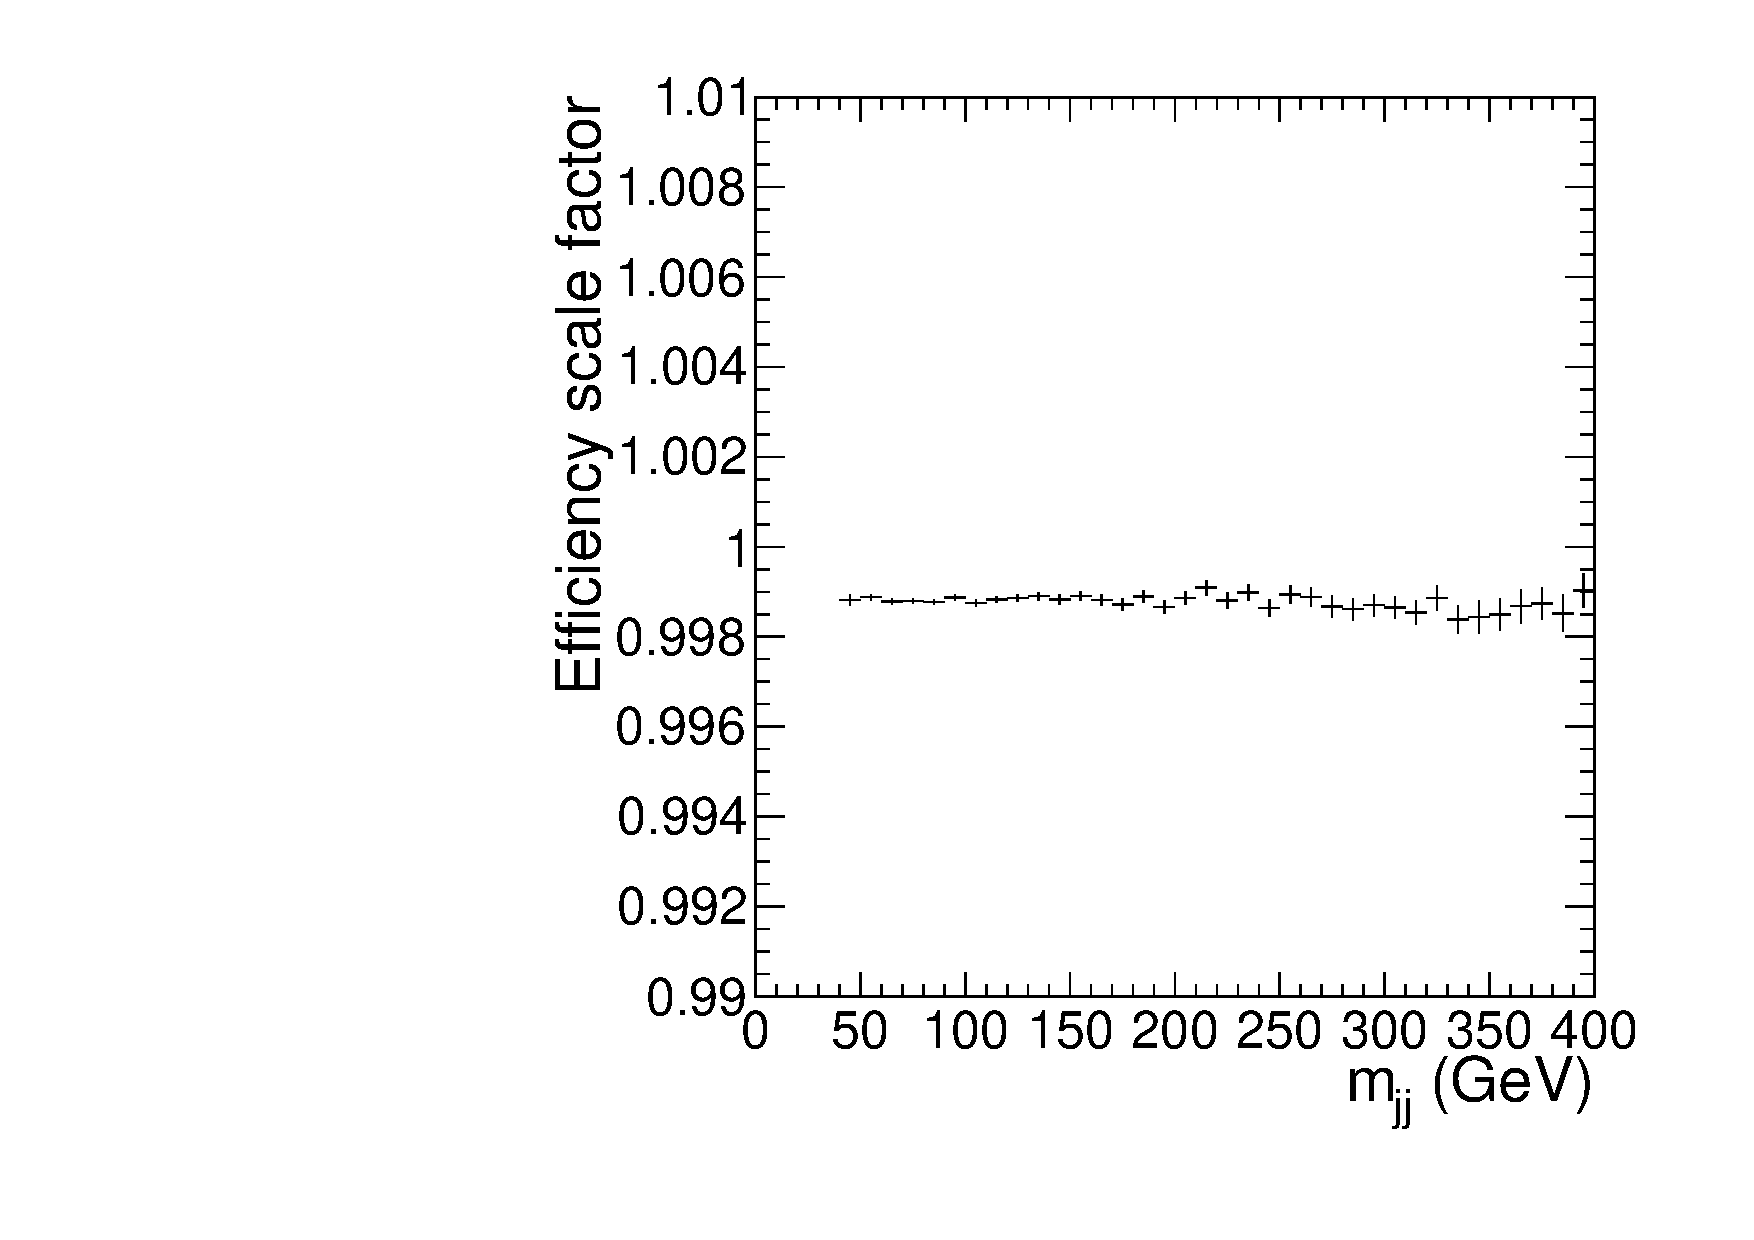
\includegraphics[width=0.48\textwidth]{figs/effPlots/fig_eff_mu_RecoToIso_ScaleFactors.pdf}
   \caption{Luminosity weighted average efficiency scale factors (data/MC) for muon isolation.}
\label{fig:muonisoeffsf}}
\end{figure}
%%%%%%%%%%%%%%%%%%%%
%%%%%%%%%%%%%%%%%%%%
\begin{figure}[h!t]
  {\centering
  \subfigure[]{
  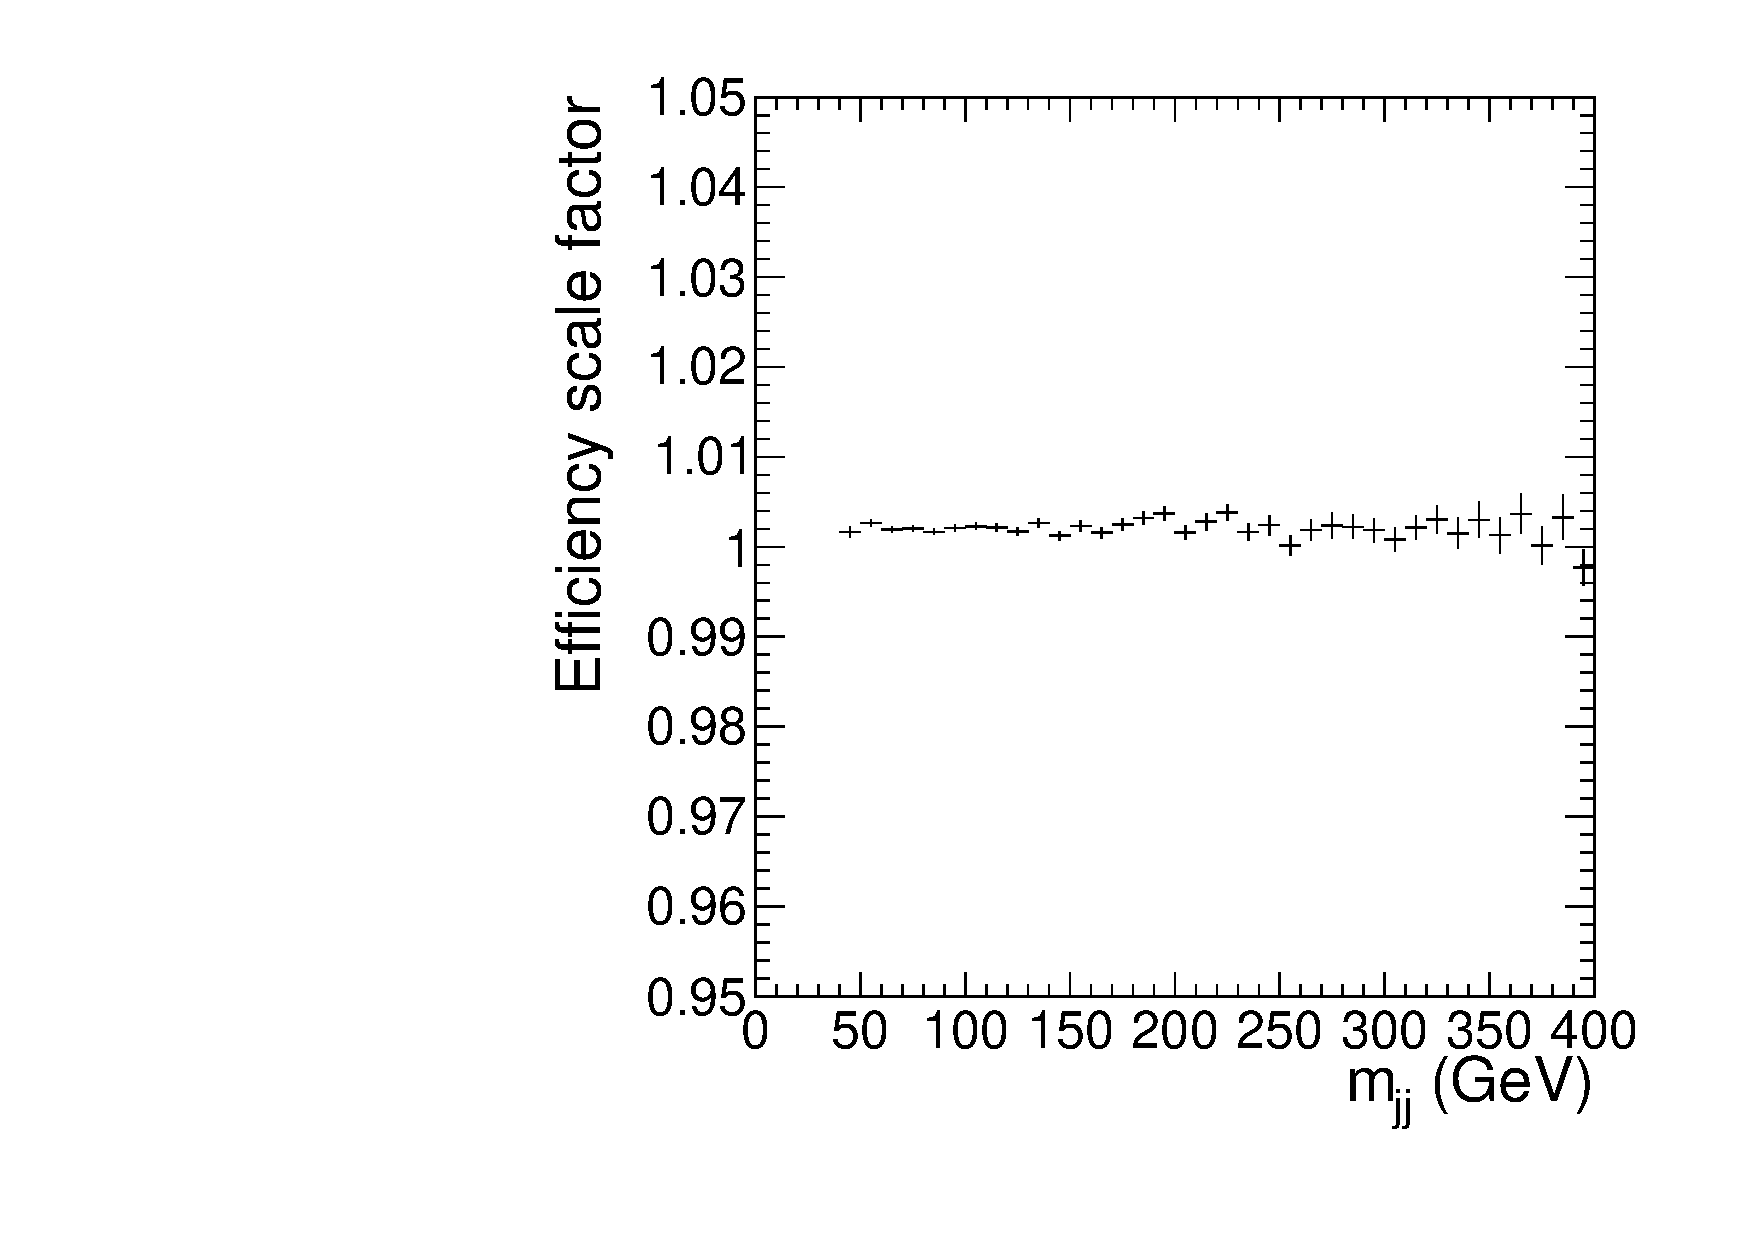
\includegraphics[width=0.48\textwidth]{figs/effPlots/fig_eff_ele_SCToReco_ScaleFactors.pdf}
   }
   \subfigure[]{
  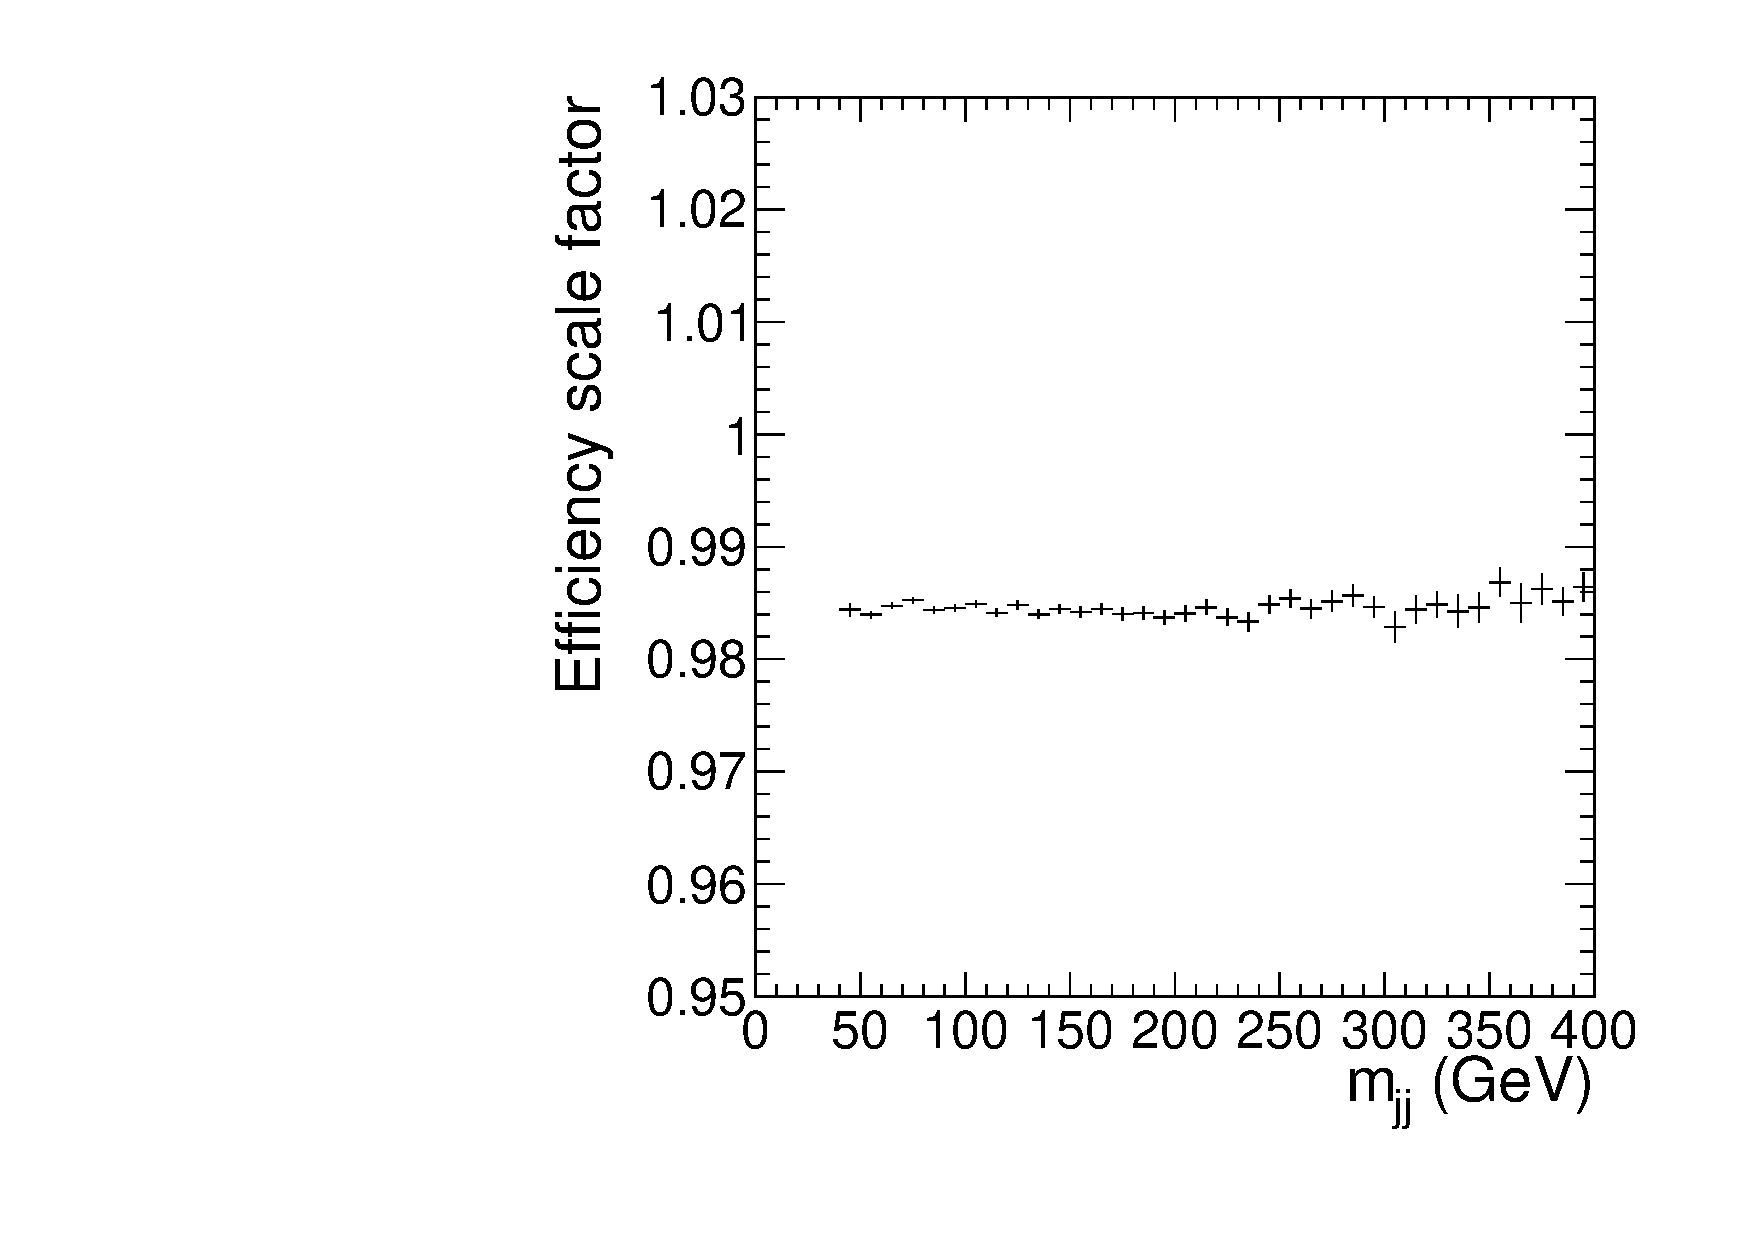
\includegraphics[width=0.48\textwidth]{figs/effPlots/fig_eff_ele_RecoToID_ScaleFactors.pdf}
   }
   \caption{Luminosity weighted average efficiency scale factors (data/MC) for electron 
   reconstruction, \textit{i.e.}, super cluster $\to$ GSF electron (a) and electron ID (b).}
\label{fig:electronRecoIDeffsf}}
\end{figure}
%%%%%%%%%%%%%%%%%%%%
%%%%%%%%%%%%%%%%%%%%%%%%%%%%%
\subsection{Electron selection (isolation and ID) scale factors}
The efficiency scale factor for electron selection is given in 
Table~\ref{tab:eleEffsRecoToWP80_ScaleFactors}.
The scale factor is statistically consistent with unity in the ECAL barrel and in the endcaps 
within systematic uncertainties.
Figure~\ref{fig:electronRecoIDeffsf} shows this scale factor variation in $m_{jj}$.
%%%%%%%%%%%
%\verbatiminput{eleEffsRecoToWP80_ScaleFactors.txt}
%%%%%%%%%%%%%%%%%%%%%%%%%%%%%
\begin{table}[bthp]
\begin{center}
  \begin{tabular}{l l c | l c}
    \hline  \hline
    $p_T$ range (GeV) & $\eta$ range  &
    $\frac{\epsilon_{\rm{Data}}}{\epsilon_{\rm{MC}}}$ & 
    $\eta$ range  & $\frac{\epsilon_{\rm{Data}}}{\epsilon_{\rm{MC}}}$\\
    \hline  
    35--40 &    -2.5-- -1.5 & 0.9545 $\pm$ 0.0055 & 1.5--2.5 & 0.9607 $\pm$ 0.0053 \\
           &    -1.5-- 0.0  & 0.9910 $\pm$ 0.0024 & 0.0--1.5 & 0.9960 $\pm$ 0.0025 \\
    \hline  
    40--45 &    -2.5-- -1.5 & 0.9661 $\pm$ 0.1567 & 1.5--2.5 & 0.9648 $\pm$ 0.0024 \\
           &    -1.5-- 0.0  & 0.9946 $\pm$ 0.0019 & 0.0--1.5 & 0.9892 $\pm$ 0.0877 \\
    \hline  
    45--50 &    -2.5-- -1.5 & 0.9672 $\pm$ 0.0050 & 1.5--2.5 & 0.9729 $\pm$ 0.0051 \\
           &    -1.5-- 0.0  & 0.9938 $\pm$ 0.0773 & 0.0--1.5 & 0.9917 $\pm$ 0.0022 \\
    \hline  
    50--200&    -2.5-- -1.5 & 0.9836 $\pm$ 0.0066 & 1.5--2.5 & 0.9813 $\pm$ 0.0068 \\
           &    -1.5-- 0.0  & 0.9915 $\pm$ 0.0030 & 0.0--1.5 & 0.9857 $\pm$ 0.0030 \\
    \hline  \hline
  \end{tabular}
\end{center}
\caption{\label{tab:eleEffsRecoToWP80_ScaleFactors}
Electron selection efficiency data/MC scale factors. The uncertainties are statistical only.
The systematic uncertainty is $\sim$1\%.}
\end{table}
%%%%%%%%%%%%%%%%%%%%%%%%%%%%%%%%%%%%%%%%%%%%%%%%%%%%%%%%%%%%%%%%%%%%
%%%%%%%%%%%%%%%%%%%%%%%%%%%%%%%%%%%%%%%%%%%%%%%%%%%%%%%%%%%%%%%%%%%%
%%%%%%%%%%%%%%%%%%%%%%%%%%%%%%%%%%%%%%%%%%%%%%%%%%%%%%%%%%%%%%%%%%%%

\section{Trigger selection}
\label{sec:trigger}
%%%%%%%%%%%%%%%%%%%%%%%%%%%%%%%
%%%%%%%%%%%%%%%%%%%%%%%%%%%%%%%
\subsection{Run2010: Runs 136033--149442}
\begin{itemize}
\item
Muon data:\\
     Mu9 OR Mu11 OR Mu13 OR Mu15\_v* OR Mu17\_v* OR Mu24\_v*  
\item
Electron data:\\   
     Ele10\_* OR Ele15\_* OR Ele17\_* 
\end{itemize}
%%%%%%%%%%%%%%%%%%%%%%%%%%%%%%%
%%%%%%%%%%%%%%%%%%%%%%%%%%%%%%%
\subsection{Run2011A: Menus 5E32 (Runs: 160404--163869), 
1E33 (Runs:165088--166967), and 1.4E33 (Runs:167039--167913)}
\begin{itemize}
\item
Muon data:\\
     IsoMu17\_v* OR Mu30\_v* \\
Note: We really needed to OR in the nonisolated muon 
trigger as it recovers about half of the offline-isolated 
muons rejected by IsoMu, increasing the trigger efficiency 
by ~5\%. 
\item
Electron data:\\   
Ele27\_CaloIdVT\_CaloIsoT\_TrkIdT\_TrkIsoT\_v* \, \, \, \textcolor{red}{5E32 epoch}\\
Ele25\_WP80\_PFMT40\_v1 \, \, \, \textcolor{red}{1E33 epoch}\\
Ele27\_WP80\_PFMT50\_v* \, \, \, \textcolor{red}{1.4E33 epoch}
\end{itemize}
%%%%%%%%%%%%%%%%%%%%%%%%%%%%%%%
%%%%%%%%%%%%%%%%%%%%%%%%%%%%%%%
\subsection{Run2011A:Menu 2E33, Runs 170249--173198}
\begin{itemize}
\item
Muon data:\\
     (IsoMu17\_v13 OR IsoMu20\_v8 OR IsoMu24\_v8) \, \, OR \, \, (Mu30\_v7 OR Mu40\_v5)\\

Note: This epoch was complicated because Mu30, IsoMu17, 
and IsoMu20 were all prescaled for brief periods, so we 
could either break it down into sub-epochs or lump them 
together. We chose the latter because it is predominantly 
IsoMu17 and the sub-epoch lumi accounting is painful.   
\item
Electron data:\\   
Ele27\_WP80\_PFMT50\_v*
\end{itemize}
%%%%%%%%%%%%%%%%%%%%%%%%%%%%%%%
%%%%%%%%%%%%%%%%%%%%%%%%%%%%%%%
\subsection{Run2011A:Menu 3E33, Runs: 173236--173692}
\begin{itemize}
\item
Muon data:\\
HLT\_IsoMu20\_v9 OR HLT\_Mu40\_eta2p1\_v1
\item
Electron data:\\
Ele27\_WP80\_PFMT50\_v* 
\end{itemize}
%%%%%%%%%%%%%%%%%%%%%%%%%%%%%%%
%%%%%%%%%%%%%%%%%%%%%%%%%%%%%%%
\subsection{Run2011B: Menu 3E33, Runs: 175832--178380}
\begin{itemize}
\item
Muon data:\\
    (IsoMu30\_eta2p1\_v3  OR IsoMu24\_eta2p1\_v3  OR IsoMu24\_v9 OR IsoMu20\_v9) \\
     OR \\  
    (Mu40\_eta2p1\_v1  OR  HLT\_Mu40\_v6)
\item
Electron data:\\  
Ele27\_WP80\_PFMT50\_v* OR Ele27\_WP70\_PFMT50\_v*
\end{itemize}
%%%%%%%%%%%%%%%%%%%%%%%%%%%%%%%
%%%%%%%%%%%%%%%%%%%%%%%%%%%%%%%
\subsection{Run2011B: Menu 5E33, Runs: 178420--180252}
\begin{itemize}
\item
Muon data:\\
       (IsoMu30\_eta2p1\_v6 OR IsoMu24\_eta2p1\_v6 OR IsoMu24\_v12 OR \\
       IsoMu30\_eta2p1\_v7 OR IsoMu24\_eta2p1\_v7 OR IsoMu24\_v13) \\
       OR \\
      (Mu40\_eta2p1\_v4 OR  Mu40\_v9) \, \, \,
      \textcolor{red}{(v1.4, 178420-179889)} \\
       OR (Mu40\_eta2p1\_v5 OR  Mu40\_v10) \, \, \,
      \textcolor{red}{(v2.2, 179959--180252)}
\item
Electron data:\\
 Ele32\_WP70\_PFMT50\_v*
\end{itemize}
%%%%%%%%%%%%%%%%%%%%%%%%%%%%%%%%%%%%%%%%%%%%%%%%%%%%%%%%%%%
\section{Trigger efficiency computation}
\label{sec:trigeff}
%%%%%%%%%%%%%%%%%%%%%%%%%%%%%%%%%%%%%%%%%%%%%%%%%%%%%%%%%%%
The efficiency of the single lepton triggers are computed 
using tag \& probe technique from Z$\to\ell^+\ell^-$ events.
The procedure is straightforward and is described in detail 
in \cite{tagnprobe} and \cite{eleceff}.
%%%%%%%%%%%%%%%%%%%%%%%%%%%%%%%%%%%%%%%%%%%%%%%%%%%%%%%%%%
\subsection{Muon trigger efficiency table}
\label{sec:trigeff_mu}
The luminosity weighted average (LWA) trigger efficiency 
for single muon triggers in data is given 
in Table~\ref{tab:muonEffsIsoToHLT_data_LP_LWA}. 
The efficiency is slowly varying
with changes in lepton transverse momentum and rapidity. 
The efficiency is typically
about 90\%.
%%%%%%%%%%%
%%%%%%%%%%%%%%%%%%%%%%%%%%%%%
\begin{table}[bthp]
\begin{center}
  \begin{tabular}{l l c | l c}
    \hline  \hline
    $p_T$ range (GeV) & $\eta$ range  & $\epsilon_{\rm{Data}}$ & 
    $\eta$ range  & $\epsilon_{\rm{Data}}$\\
    \hline  
    25--30 &    -2.1-- -1.5 &   0.8490 $\pm$ 0.0032  & 1.5--2.1   & 0.8457 $\pm$ 0.0033 \\
           &    -1.5-- -1.0 &   0.8725 $\pm$ 0.0032  & 1.0--1.5   & 0.8628 $\pm$ 0.0032 \\
           &    -1.0-- -0.5 &   0.9057 $\pm$ 0.0026  & 0.5--1.0   & 0.8999 $\pm$ 0.0027 \\
           &    -0.5--  0.0 &   0.9211 $\pm$ 0.0022  & 0.0--0.5   & 0.9251 $\pm$ 0.0022 \\
    \hline  
    30--35 &    -2.1-- -1.5 &   0.8797 $\pm$ 0.0031  & 1.5--2.1   & 0.8768 $\pm$ 0.0031 \\
           &    -1.5-- -1.0 &   0.9136 $\pm$ 0.0030  & 1.0--1.5   & 0.9016 $\pm$ 0.0031 \\
           &    -1.0-- -0.5 &   0.9397 $\pm$ 0.0025  & 0.5--1.0   & 0.9387 $\pm$ 0.0025 \\
           &    -0.5--  0.0 &   0.9579 $\pm$ 0.0022  & 0.0--0.5   & 0.9556 $\pm$ 0.0021 \\
    \hline  
    35--40 &    -2.1-- -1.5 &   0.8816 $\pm$ 0.0027  & 1.5--2.1   & 0.8894 $\pm$ 0.0026 \\
           &    -1.5-- -1.0 &   0.9142 $\pm$ 0.0025  & 1.0--1.5   & 0.9008 $\pm$ 0.0026 \\
           &    -1.0-- -0.5 &   0.9385 $\pm$ 0.0022  & 0.5--1.0   & 0.9385 $\pm$ 0.0021 \\
           &    -0.5--  0.0 &   0.9571 $\pm$ 0.0019  & 0.0--0.5   & 0.9546 $\pm$ 0.0019 \\
    \hline  
    40--45 &    -2.1-- -1.5 &   0.8878 $\pm$ 0.0024  & 1.5--2.1   & 0.8902 $\pm$ 0.0024 \\
           &    -1.5-- -1.0 &   0.9221 $\pm$ 0.0021  & 1.0--1.5   & 0.9076 $\pm$ 0.0022 \\
           &    -1.0-- -0.5 &   0.9443 $\pm$ 0.0020  & 0.5--1.0   & 0.9457 $\pm$ 0.0019 \\
           &    -0.5--  0.0 &   0.9622 $\pm$ 0.0018  & 0.0--0.5   & 0.9617 $\pm$ 0.0018 \\
    \hline  
    45--50 &    -2.1-- -1.5 &   0.8922 $\pm$ 0.0029  & 1.5--2.1   & 0.8934 $\pm$ 0.0028 \\
           &    -1.5-- -1.0 &   0.9202 $\pm$ 0.0027  & 1.0--1.5   & 0.9069 $\pm$ 0.0027 \\
           &    -1.0-- -0.5 &   0.9458 $\pm$ 0.0024  & 0.5--1.0   & 0.9437 $\pm$ 0.0025 \\
           &    -0.5--  0.0 &   0.9625 $\pm$ 0.0023  & 0.0--0.5   & 0.9615 $\pm$ 0.0023 \\
    \hline  
    50--200&    -2.1-- -1.5 &   0.8920 $\pm$ 0.0031  & 1.5--2.1   & 0.8903 $\pm$ 0.0032 \\
           &    -1.5-- -1.0 &   0.9178 $\pm$ 0.0030  & 1.0--1.5   & 0.9041 $\pm$ 0.0030 \\
           &    -1.0-- -0.5 &   0.9419 $\pm$ 0.0027  & 0.5--1.0   & 0.9424 $\pm$ 0.0028 \\
           &    -0.5--  0.0 &   0.9606 $\pm$ 0.0026  & 0.0--0.5   & 0.9604 $\pm$ 0.0025 \\
    \hline  \hline
  \end{tabular}
\end{center}
\caption{\label{tab:muonEffsIsoToHLT_data_LP_LWA}
Muon trigger efficiency in data (luminosity 
weighted average). The uncertainties are statistical only.
The systematic uncertainty is $\sim$1\%.}
\end{table}
%%%%%%%%%%%%
%%%%%%%%%%%
\subsection{Electron trigger efficiency table}
\label{sec:trigeff_eleEle27}
The luminosity weighted average trigger efficiency for the 
electron triggers is shown in
Table~\ref{tab:eleEffsHLTEle}.  
The value is typically about 99\% in the barrel and 92--97\% in 
the endcaps, and is weakly dependent on the electron
$p_T$ and pseudorapidity.
The efficiency for the W transverse mass leg is shown in 
Table~\ref{tab:eleEffsHLTEleMT}.  
The average value is 91.74 $\pm$ 0.07\% with a large variation depending on 
whether the electron is in the barrel or endcaps.
Fortunately for us this is just an overall scaling effect in the 
$m_{jj}$ and $m_{\ell\nu jj}$ distributions.
The impact of this turnon on the dijet invariant mass or WW invariant mass templates
(used in Higgs analysis) is negligible as shown in 
Fig~\ref{fig:singleElehlteffMT}.
%%%%%%%%%%%
%%%%%%%%%%%%%%%%%%%%%%%%%%%%%
\begin{table}[bthp]
\begin{center}
  \begin{tabular}{l l c | l c}
    \hline  \hline
    $p_T$ range (GeV) & $\eta$ range  & $\epsilon_{\rm{Data}}$ & 
    $\eta$ range  & $\epsilon_{\rm{Data}}$\\
    \hline  
    35--40 &    -2.5-- -1.5 & 0.92 $\pm$ 0.01 & 1.5--2.5 & 0.91 $\pm$ 0.01 \\
           &    -1.5-- 0.0  & 0.99 $\pm$ 0.01 & 0.0--1.5 & 0.99 $\pm$ 0.01 \\
    \hline  
    40--45 &    -2.5-- -1.5 & 0.96 $\pm$ 0.01 & 1.5--2.5 & 0.96 $\pm$ 0.01 \\
           &    -1.5-- 0.0  & 0.99 $\pm$ 0.01 & 0.0--1.5 & 0.99 $\pm$ 0.01 \\
    \hline  
    45--50 &    -2.5-- -1.5 & 0.97 $\pm$ 0.01 & 1.5--2.5 & 0.97 $\pm$ 0.01 \\
           &    -1.5-- 0.0  & 0.99 $\pm$ 0.01 & 0.0--1.5 & 0.99 $\pm$ 0.01 \\
    \hline  
    50--200&    -2.5-- -1.5 & 0.93 $\pm$ 0.01 & 1.5--2.5 & 0.92 $\pm$ 0.01 \\
           &    -1.5-- 0.0  & 0.98 $\pm$ 0.01 & 0.0--1.5 & 0.98 $\pm$ 0.01 \\
    \hline  \hline
  \end{tabular}
\end{center}
\caption{\label{tab:eleEffsHLTEle}
Electron trigger efficiency in data (luminosity weighted average). 
The statistical uncertainties are negligible.
The quoted uncertainties are systematic.}
\end{table}
%%%%%%%%%%%%%%%%%%%%%%%%%%%%%
\begin{table}[bthp]
\begin{center}
  \begin{tabular}{l l c | l c}
    \hline  \hline
    Offline $m_T$ range (GeV) & electron $\eta$ range  & $\epsilon_{\rm{Data}}$ & 
    electron $\eta$ range  & $\epsilon_{\rm{Data}}$\\
    \hline  
     50--55 &	-2.5-- -1.5 & 0.3580 $\pm$ 0.0167 &	+1.5--2.5 & 0.3580 $\pm$ 0.0167 \\ 
            &	-1.5--0.0 & 0.7315 $\pm$ 0.0129  &	+0.0--1.5 & 0.7315 $\pm$ 0.0129 \\
    \hline
     55--60 &	-2.5-- -1.5 & 0.4796 $\pm$ 0.0165  &	+1.5--2.5 & 0.4796 $\pm$ 0.0165 \\ 
            &	-1.5--0.0 & 0.8151 $\pm$ 0.0112  &	+0.0--1.5 & 0.8151 $\pm$ 0.0112 \\ 
    \hline
     60--65 &	-2.5-- -1.5 & 0.6073 $\pm$ 0.0144  &	+1.5--2.5 & 0.6073 $\pm$ 0.0144 \\ 
            &	-1.5--0.0 & 0.9035 $\pm$ 0.0085  &	+0.0--1.5 & 0.9035 $\pm$ 0.0085 \\ 
    \hline
     65--70 &	-2.5-- -1.5 & 0.7473 $\pm$ 0.0100 &	+1.5--2.5 & 0.7473 $\pm$ 0.0100 \\  
            &	-1.5--0.0 & 0.9548 $\pm$ 0.0047  &	+0.0--1.5 & 0.9548 $\pm$ 0.0047  \\
    \hline
     70--75 &	-2.5-- -1.5 & 0.8256 $\pm$ 0.0069  &	+1.5--2.5 & 0.8256 $\pm$ 0.0069 \\ 
            &	-1.5--0.0 & 0.9756 $\pm$ 0.0036  &	+0.0--1.5 & 0.9756 $\pm$ 0.0036 \\ 
    \hline
     75--80 &	-2.5-- -1.5 & 0.8711 $\pm$ 0.0060  &	+1.5--2.5 & 0.8711 $\pm$ 0.0060 \\ 
            &	-1.5--0.0 & 0.9866 $\pm$ 0.0034  &	+0.0--1.5 & 0.9866 $\pm$ 0.0034 \\
    \hline
     80--85 &	-2.5-- -1.5 & 0.9047 $\pm$ 0.0059  &	+1.5--2.5 & 0.9047 $\pm$ 0.0059  \\
            &	-1.5--0.0 & 0.9934 $\pm$ 0.0034  &	+0.0--1.5 & 0.9934 $\pm$ 0.0034 \\ 
    \hline
     85--90 &	-2.5-- -1.5 & 0.9308 $\pm$ 0.0061  &	+1.5--2.5 & 0.9308 $\pm$ 0.0061 \\ 
            &	-1.5--0.0 & 0.9958 $\pm$ 0.0038  &	+0.0--1.5 & 0.9958 $\pm$ 0.0038  \\
    \hline
     90--95 &	-2.5-- -1.5 & 0.9415 $\pm$ 0.0068  &	+1.5--2.5 & 0.9415 $\pm$ 0.0068  \\
            &	-1.5--0.0 & 0.9975 $\pm$ 0.0046  &	+0.0--1.5 & 0.9975 $\pm$ 0.0046  \\
    \hline
     95--100 &	-2.5-- -1.5 & 0.9441 $\pm$ 0.0080 &	+1.5--2.5 & 0.9441 $\pm$ 0.0080  \\ 
             &	-1.5--0.0 & 0.9973 $\pm$ 0.0057  &	+0.0--1.5 & 0.9973 $\pm$ 0.0057  \\
    \hline
     100--110 &	-2.5-- -1.5 & 0.9358 $\pm$ 0.0074  &	+1.5--2.5 & 0.9358 $\pm$ 0.0074 \\ 
              &	-1.5--0.0 & 0.9980 $\pm$ 0.0059  &	+0.0--1.5 & 0.9980 $\pm$ 0.0059 \\ 
    \hline
     110--120 &	-2.5-- -1.5 & 0.9120 $\pm$ 0.0109  &	+1.5--2.5 & 0.9120 $\pm$ 0.0109 \\
              &	-1.5--0.0 & 0.9963 $\pm$ 0.0101  &	+0.0--1.5 & 0.9963 $\pm$ 0.0101  \\
    \hline
     120--140 &	-2.5-- -1.5 & 0.8721 $\pm$ 0.0117  &	+1.5--2.5 & 0.8721 $\pm$ 0.0117  \\
              &	-1.5--0.0 & 0.9950 $\pm$ 0.0123  &	+0.0--1.5 & 0.9950 $\pm$ 0.0123  \\
    \hline
     140--180 &	-2.5-- -1.5 & 0.8311 $\pm$ 0.0153  &	+1.5--2.5 & 0.8311 $\pm$ 0.0153  \\
              &	-1.5--0.0 & 0.9899 $\pm$ 0.0171  &	+0.0--1.5 & 0.9899 $\pm$ 0.0171  \\
    \hline
     180--240 &	-2.5-- -1.5 & 0.8011 $\pm$ 0.0266  &	+1.5--2.5 & 0.8011 $\pm$ 0.0266  \\
              &	-1.5--0.0 & 0.9915 $\pm$ 0.0290  &	+0.0--1.5 & 0.9915 $\pm$ 0.0290  \\
    \hline
     240--300 &	-2.5-- -1.5 & 0.8110 $\pm$ 0.0710  &	+1.5-+2.5 & 0.8110 $\pm$ 0.0710 \\ 
              &	-1.5--0.0 & 1.0000 $\pm$ 0.0829  &	+0.0--1.5 & 1.0000 $\pm$ 0.0829  \\
    \hline  \hline
  \end{tabular}
\end{center}
\caption{\label{tab:eleEffsHLTEleMT}
Efficiency for W transverse mass cut ($> 50$~GeV for most epochs) in HLT 
for single electron trigger in data (luminosity weighted average). 
The uncertainties are all inclusive.}
\end{table}
%%%%%%%%%%%%%%%%%%%%%%%%%%%%%
%%%%%%%%%%%%%%%%%%%%
\begin{figure}[h!t]
  {\centering
  \subfigure[]{
  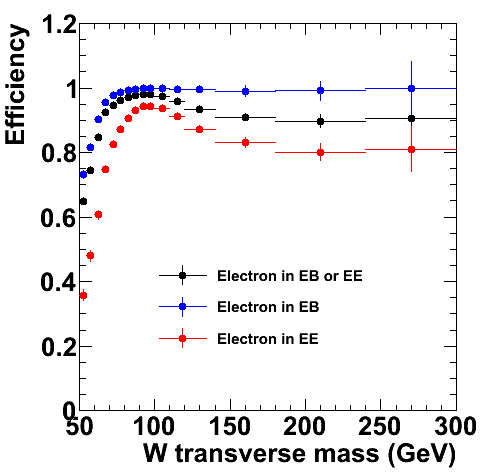
\includegraphics[width=0.48\textwidth]{figs/effPlots/WMt50TriggerEfficiency.png}
  }   
\vspace*{1mm} \\
  \subfigure[]{
  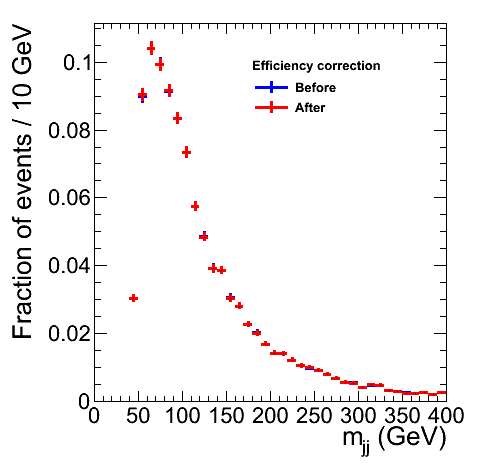
\includegraphics[width=0.48\textwidth]{figs/effPlots/fig_eff_HLTWMT50_template.png}
   }
   \subfigure[]{
   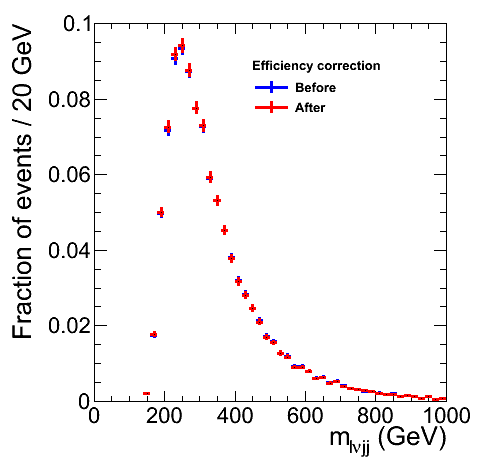
\includegraphics[width=0.48\textwidth]{figs/effPlots/fig_eff_HLTWMT50_template4body.png}
   }
   \caption{Luminosity weighted average trigger efficiency in the 
   %first 200 pb${}^{-1}$ of 2011 electron data (single electron $HLT_Ele27$) 
     electron data for W transverse mass leg as a function 
   of $m_{jj}$ (a). 
   The effect of this efficiency correction on W+jets shape is shown for 
   $m_{jj}$ (b) and $m_{\ell\nu jj}$ (c) templates.}
\label{fig:singleElehlteffMT}}
\end{figure}
%%%%%%%%%%%%%%%%%%%%
%%%%%%%%%%%%%%%%%%%%%%%%%%%%%%%%%%%%%%%%%%%%%%%%%%%%%%%%%%%%%%%%%%%%
%%%%%%%%%%%%%%%%%%%%%%%%%%%%%%%%%%%%%%%
\subsection{Effect of trigger efficiency on shapes}
As shown in Figs.~\ref{fig:muonhlteff}-\ref{fig:singleElehlteff}, 
the overall trigger efficiency with respect to the analysis selection criteria
is uniform~\footnote{Except for the Electron+2Jet+MHT cross-object trigger, for 
which the efficiency has significant variations in the kinematic variables of 
interest. We are currently working to take these variations into account.} 
across various trigger epochs within the systematic uncertainty. 
Since the trigger efficiency is flat, it does not alter the 
di-jet mass shape, other than introducing a 
global factor that will be absorbed in the normalization of the fit.
Therefore, we have followed the strategy not to apply any trigger 
correction in Monte Carlo. 
We compute the systematic error due to the efficiency 
uncertainty by recomputing the envelope for the MC shape templates 
and propagating these templates to the $m_{jj}$ fit as described in 
a later section. 

%%%%%%%%%%%%%%%%%%%%
\begin{figure}[h!t]
  {\centering
  \subfigure[]{
  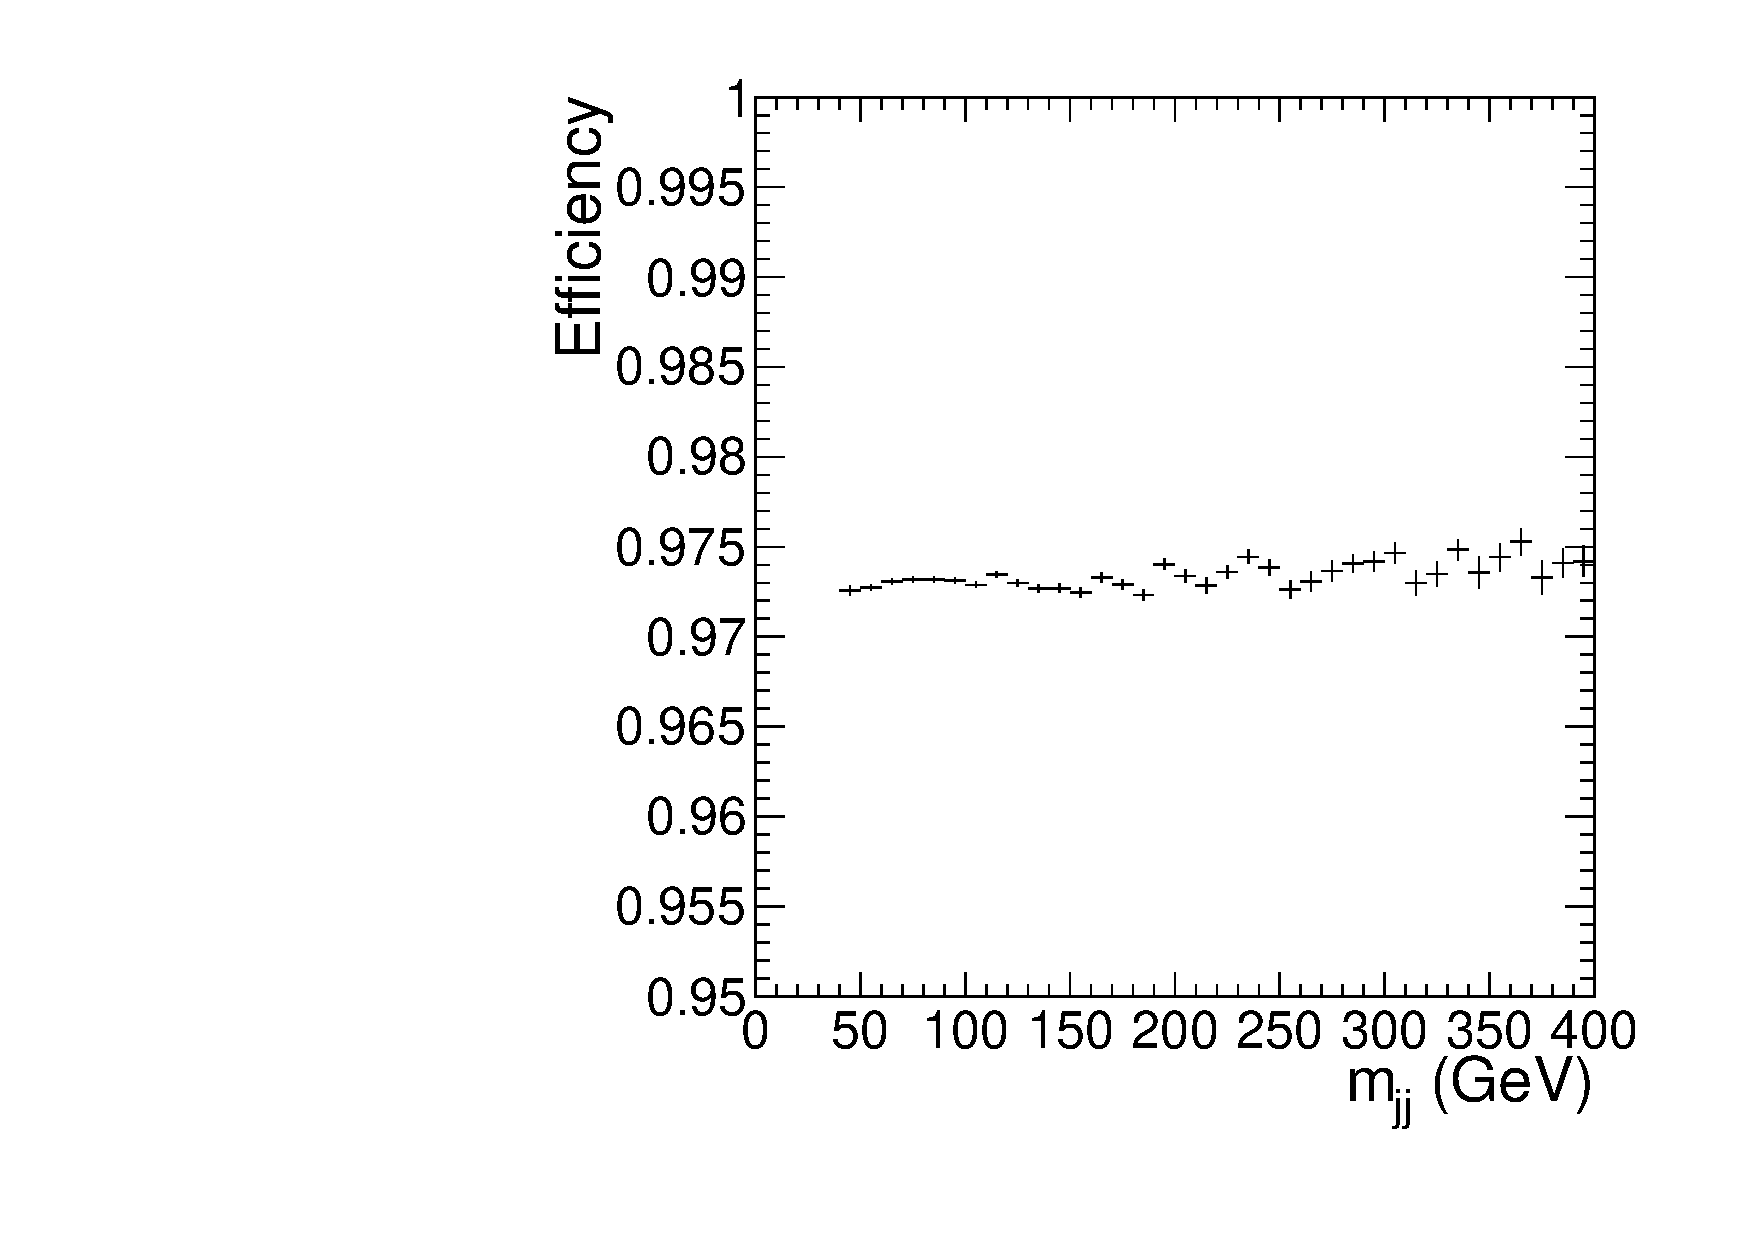
\includegraphics[width=0.48\textwidth]{figs/effPlots/fig_eff_HLTMu.pdf}
  }   
\vspace*{1mm} \\
  \subfigure[]{
  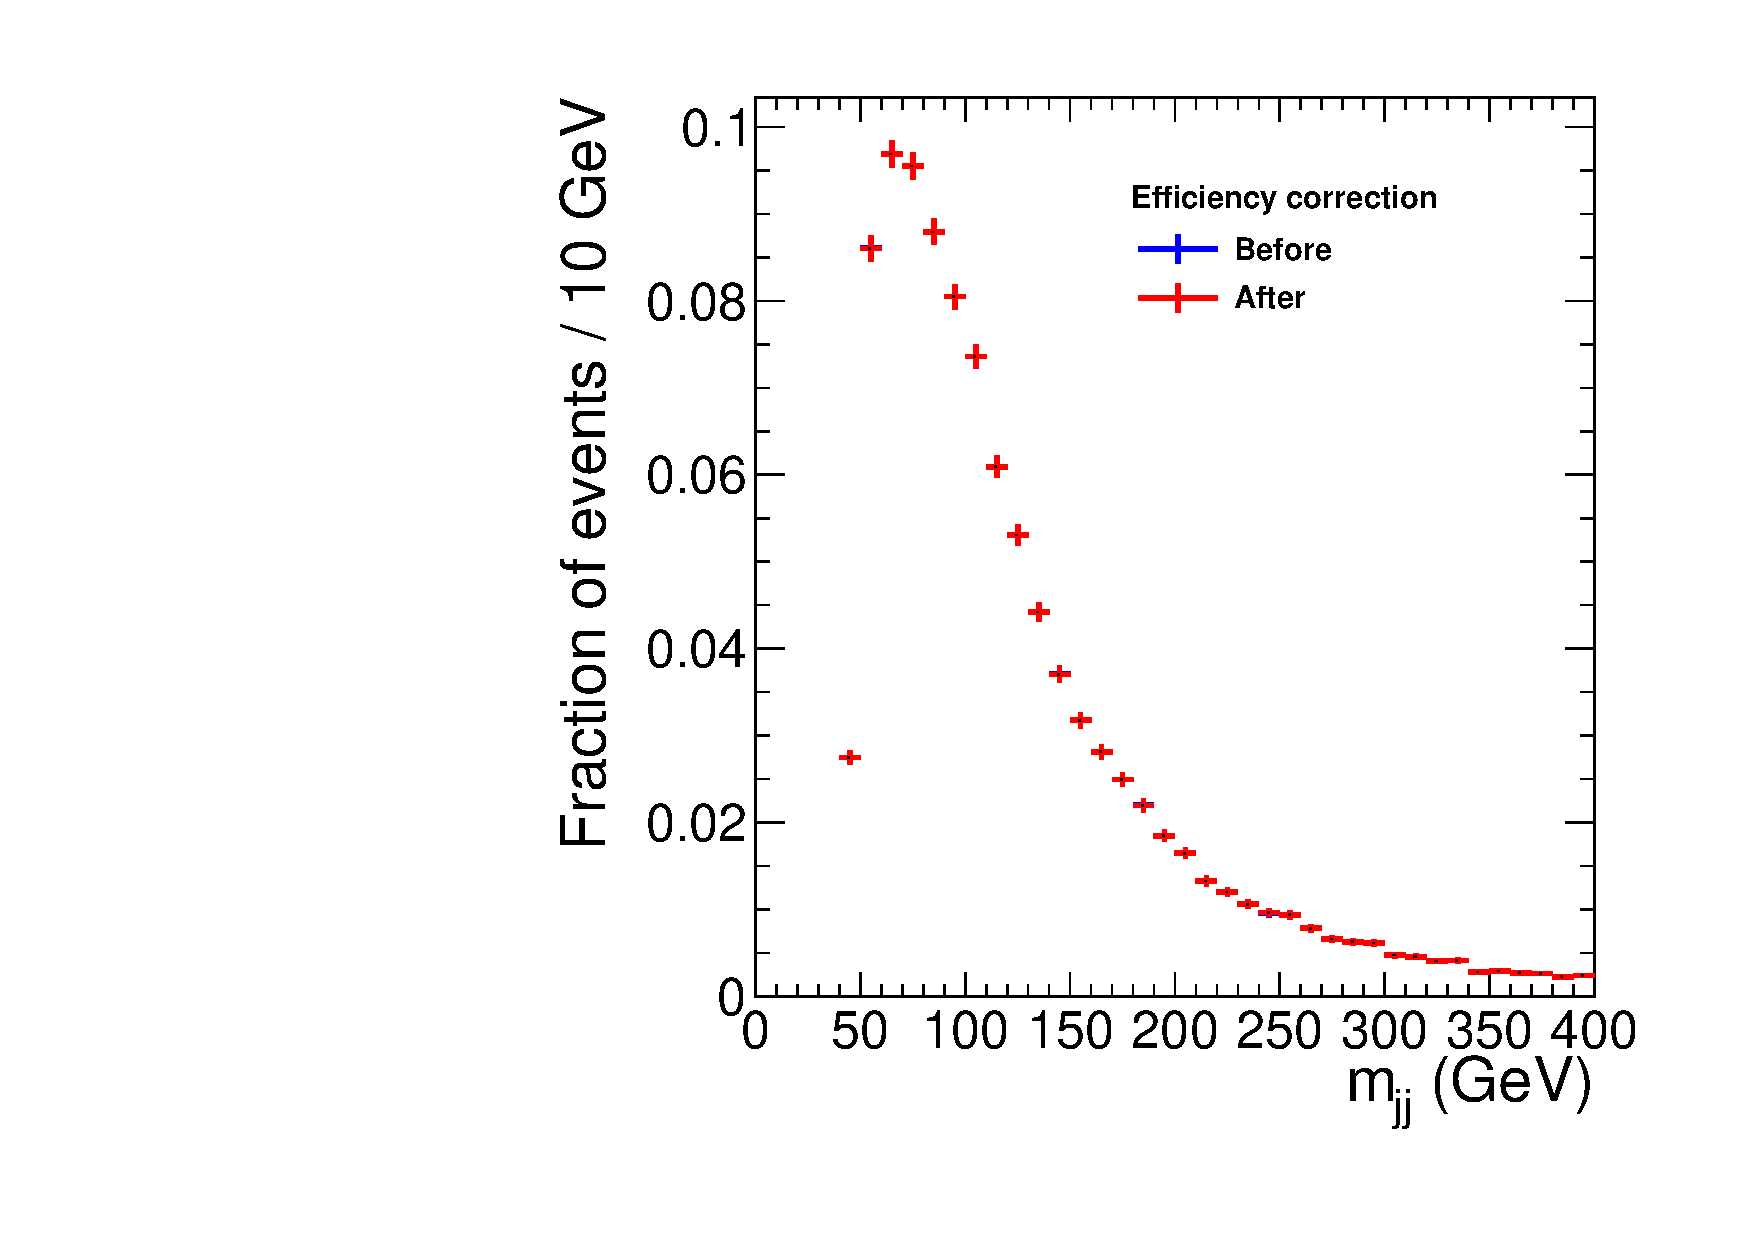
\includegraphics[width=0.48\textwidth]{figs/effPlots/fig_eff_HLTMu_template.pdf}
   }
   \subfigure[]{
   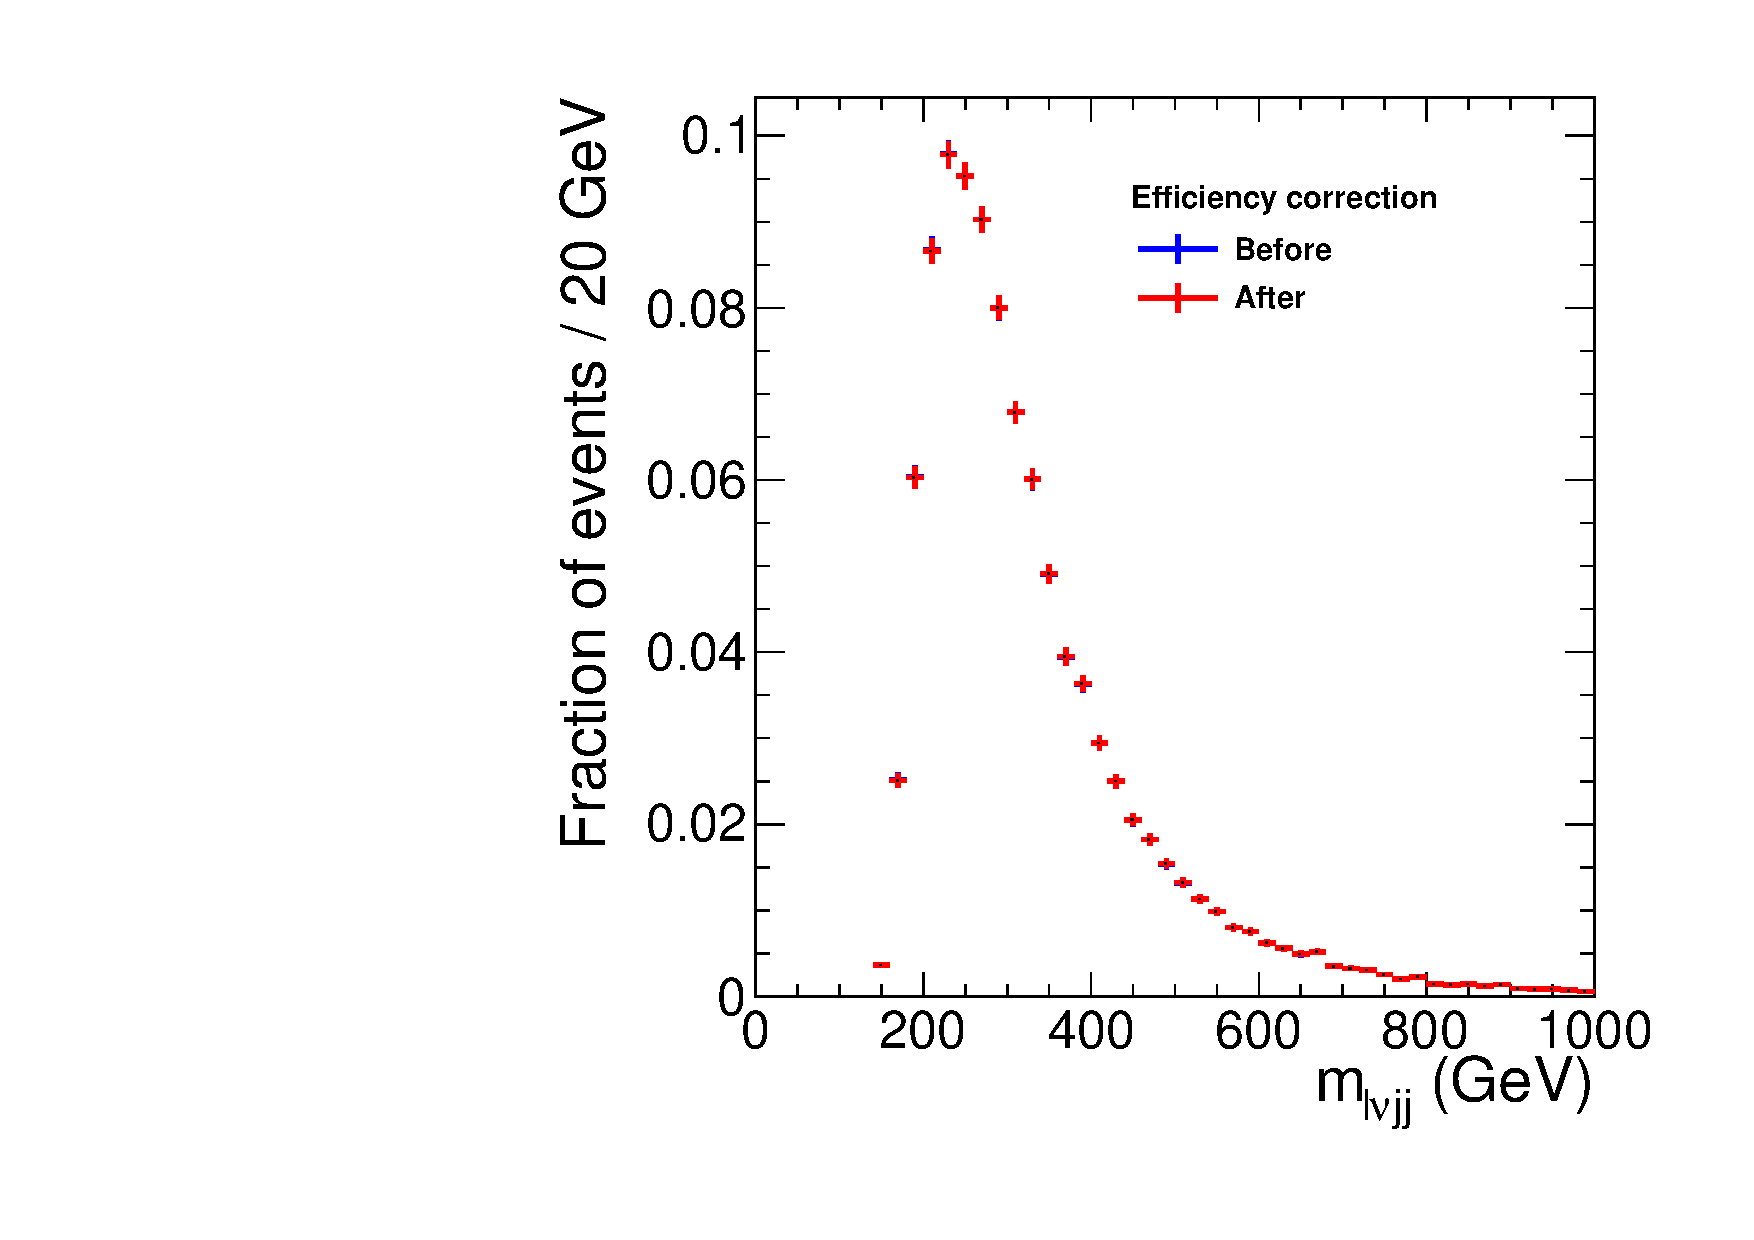
\includegraphics[width=0.48\textwidth]{figs/effPlots/fig_eff_HLTMu_template4body.pdf}
   }
   \caption{Luminosity weighted average trigger efficiency in the muon data as a function 
   of $m_{jj}$ (a). 
   The effect of this efficiency correction on W+jets shape is shown for 
   $m_{jj}$ (b) and $m_{\ell\nu jj}$ (c) templates.}
\label{fig:muonhlteff}}
\end{figure}
%%%%%%%%%%%%%%%%%%%%
%%%%%%%%%%%%%%%%%%%%
\begin{figure}[h!t]
  {\centering
  \subfigure[]{
  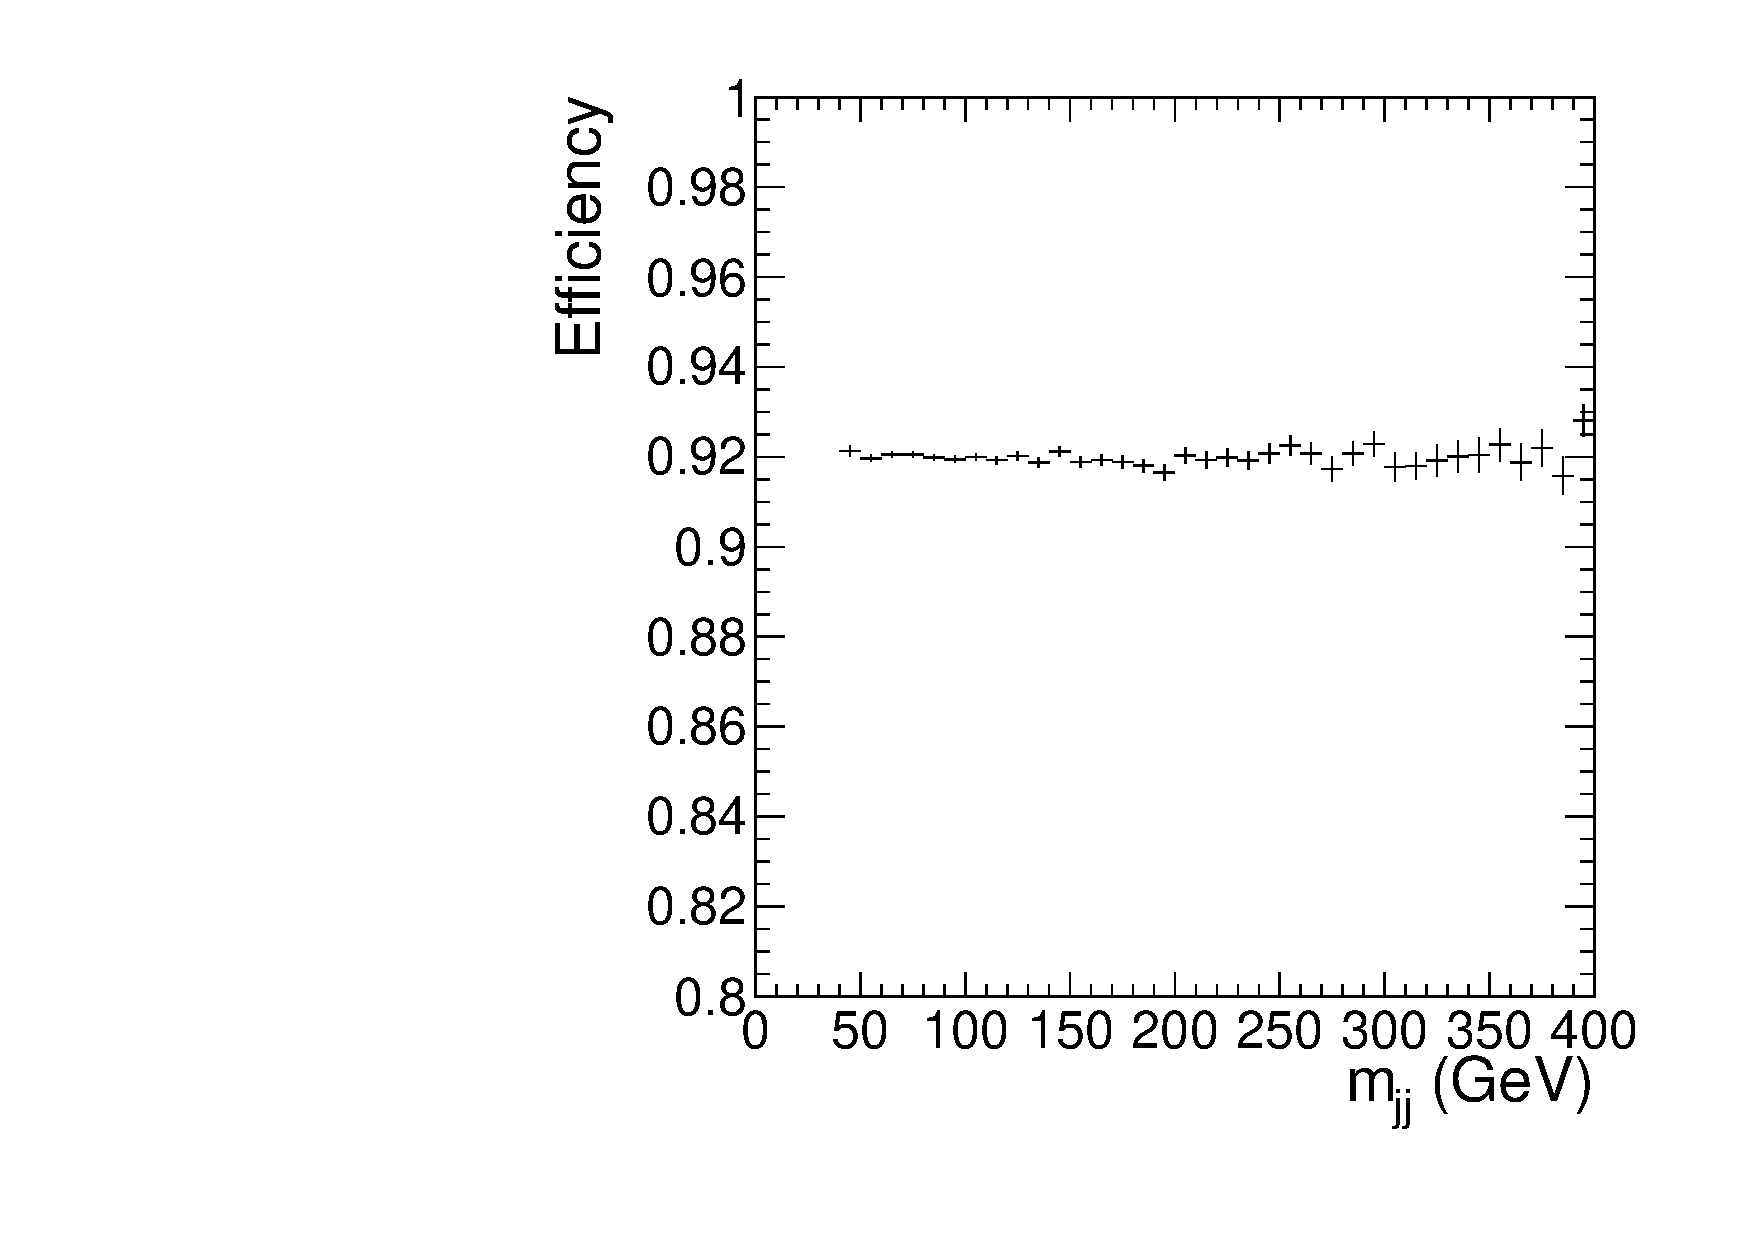
\includegraphics[width=0.48\textwidth]{figs/effPlots/fig_eff_HLTEle27_May10ReReco.pdf}
  }   
\vspace*{1mm} \\
  \subfigure[]{
  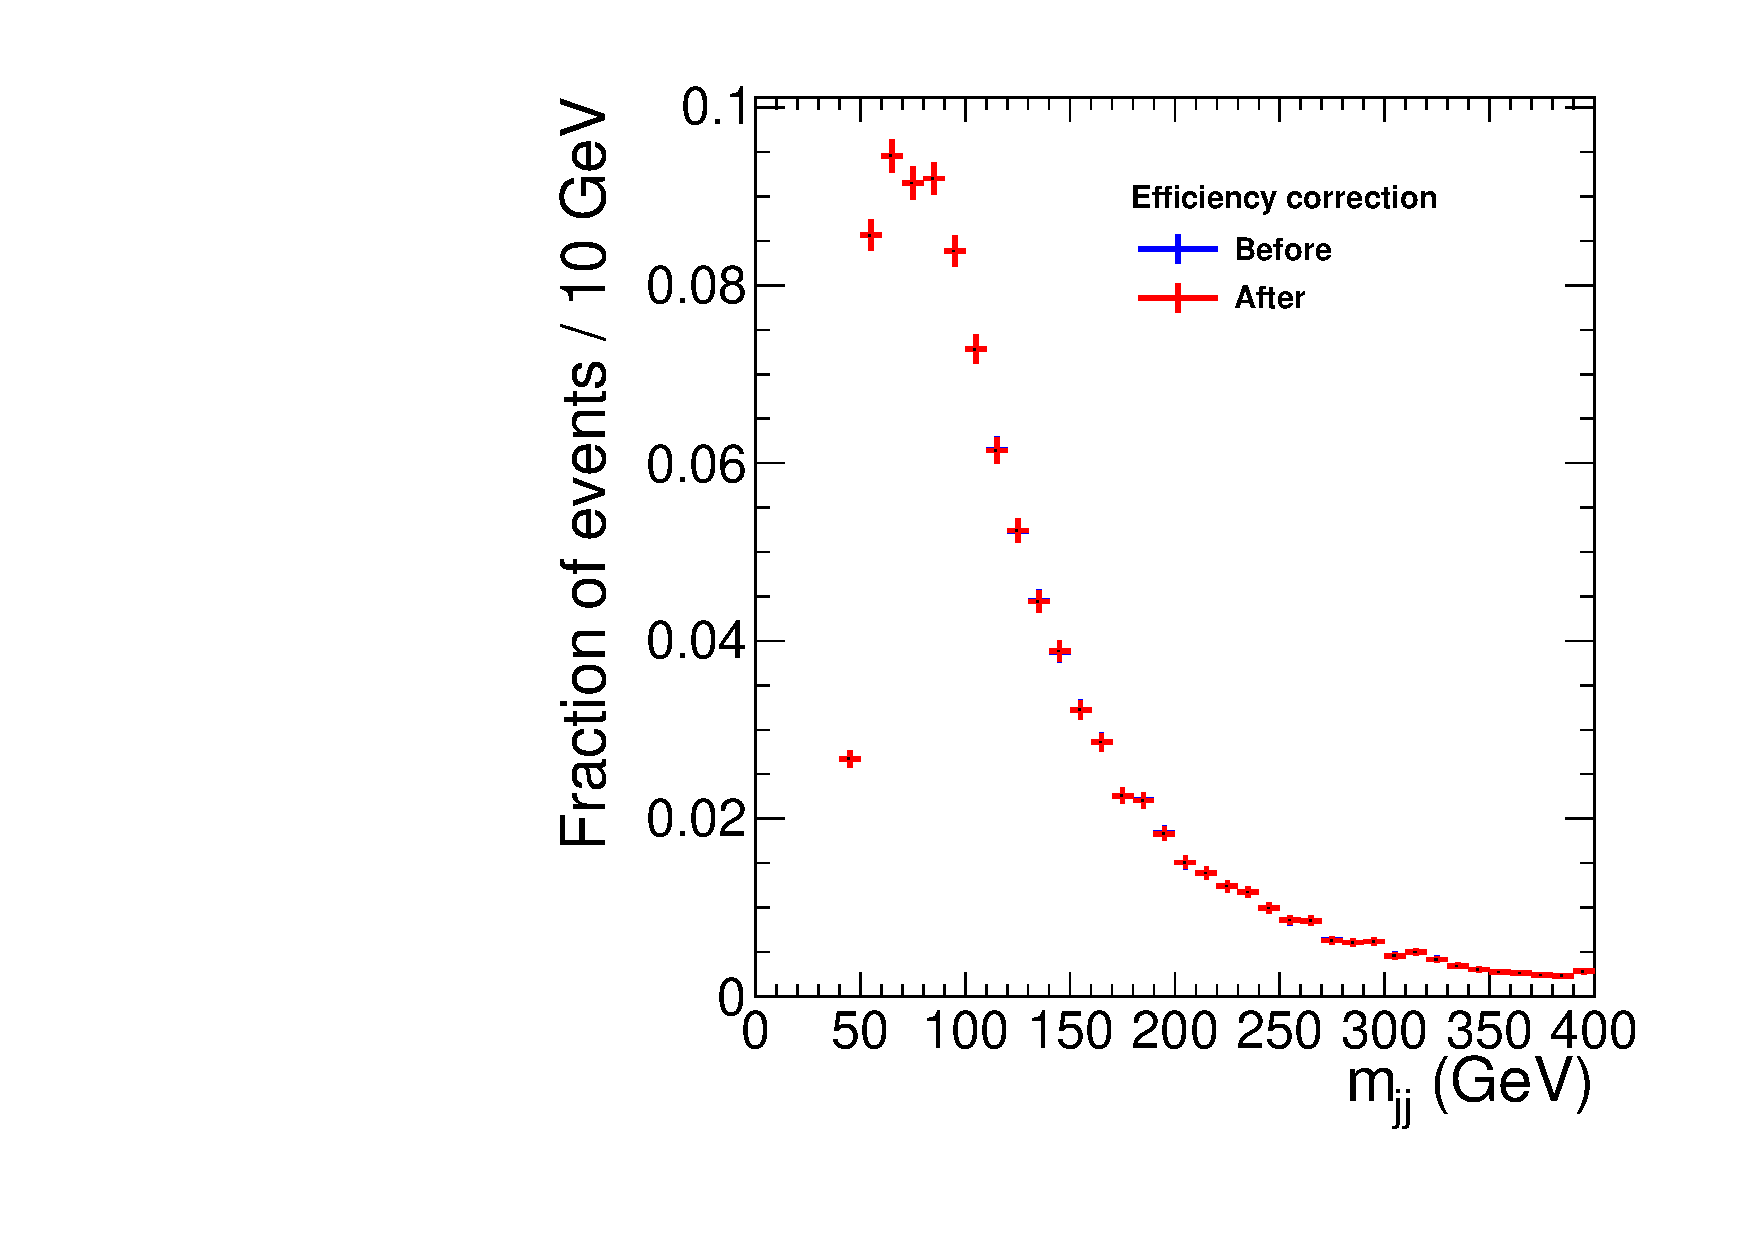
\includegraphics[width=0.48\textwidth]{figs/effPlots/fig_eff_HLTEle27_May10ReReco_template.pdf}
   }
   \subfigure[]{
   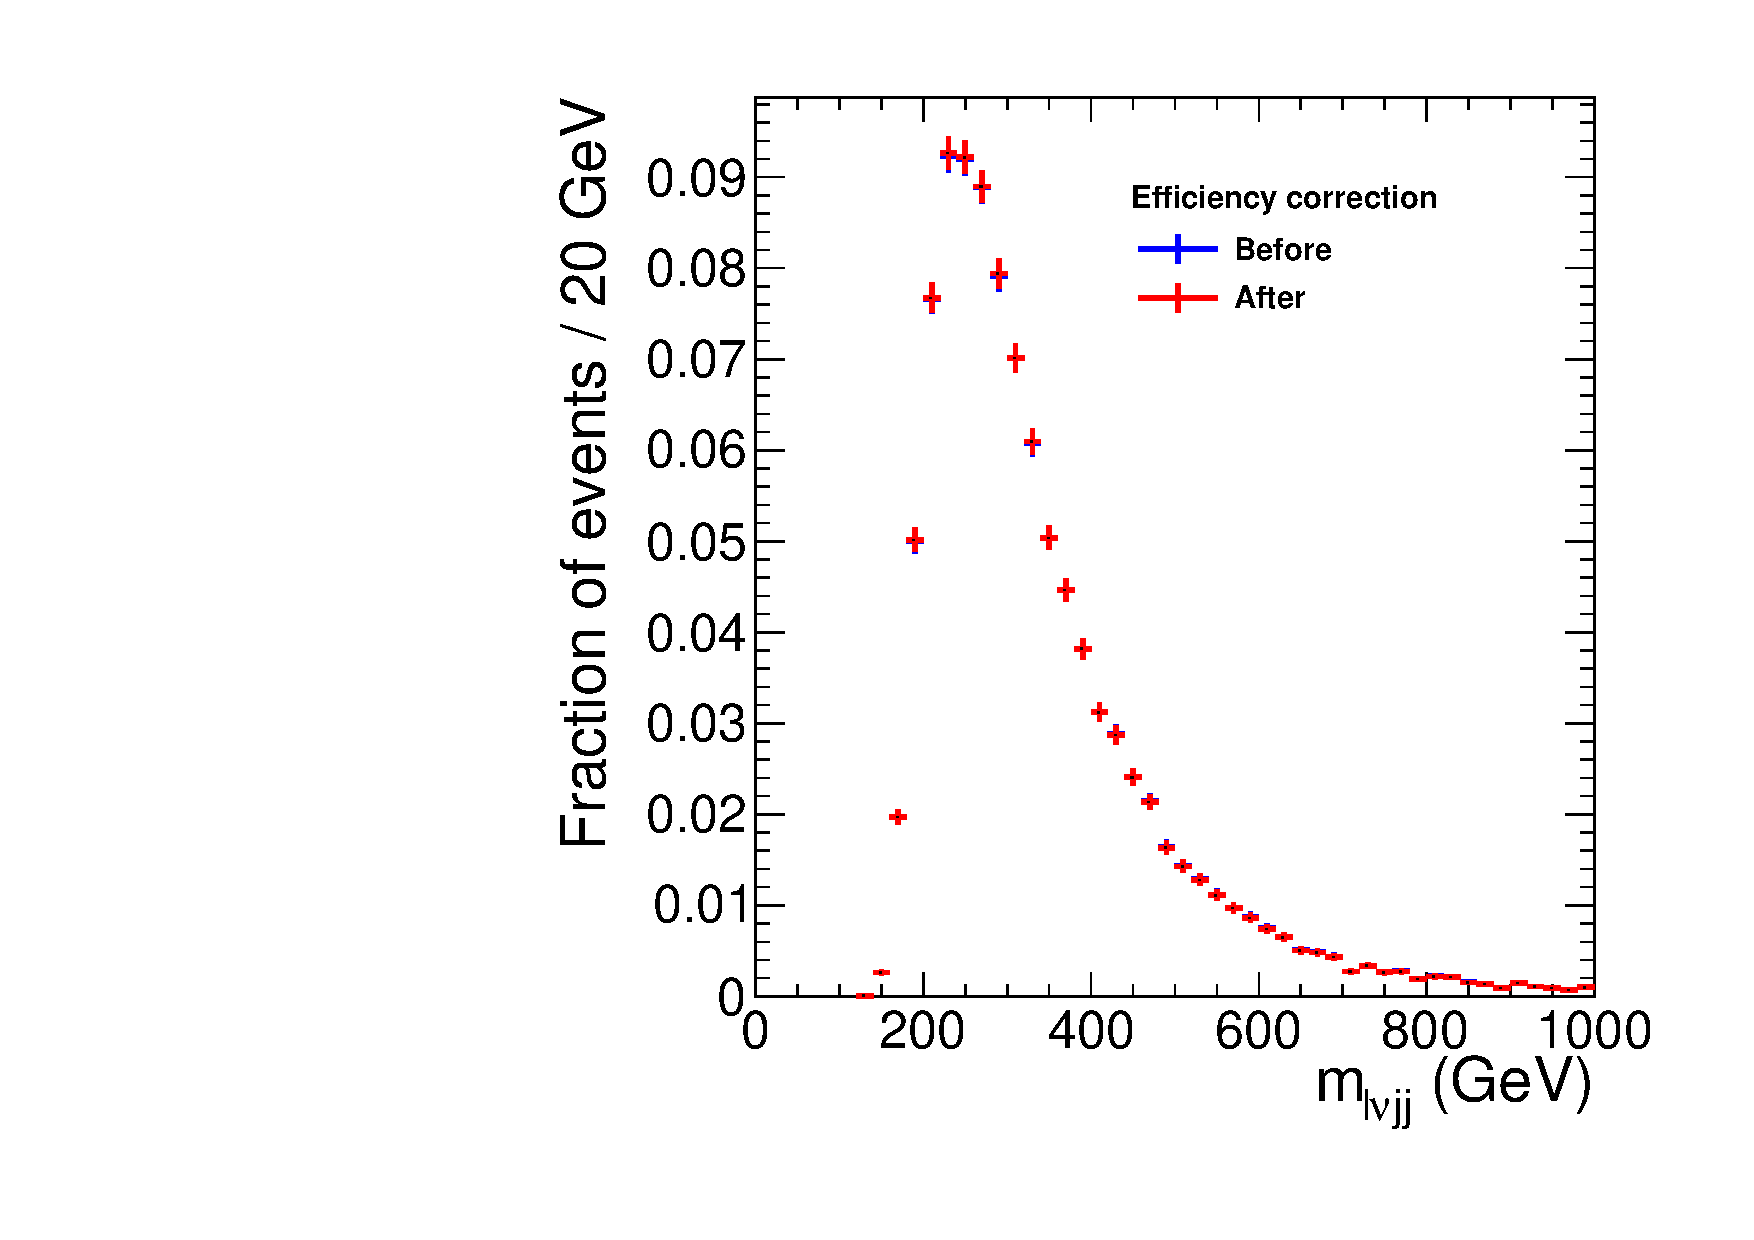
\includegraphics[width=0.48\textwidth]{figs/effPlots/fig_eff_HLTEle27_May10ReReco_template4body.pdf}
   }
   \caption{Luminosity weighted average trigger efficiency in the 
   %first 200 pb${}^{-1}$ of 2011 electron data (single electron $HLT_Ele27$) 
     electron data 
   as a function 
   of $m_{jj}$ (a). 
   The effect of this efficiency correction on W+jets shape is shown for 
   $m_{jj}$ (b) and $m_{\ell\nu jj}$ (c) templates.}
\label{fig:singleElehlteff}}
\end{figure}
%%%%%%%%%%%%%%%%%%%%

\par
To further crosscheck the impact of the trigger correction on the
$m_{jj}$ shape, we applied a single lepton trigger requirement in the MC 
simulation (chosen by an "OR" of different single muon or single 
electron paths present in the Summer11 Monte Carlo production)
and re-derived the shapes.
The rationale is that, although the trigger implemented 
for the MC does not perfectly mimic the actual trigger, it captures
the major kinematic effects on distributions. 
However, the specific trigger paths used to select events are 
distinctly different in data and Monte Carlo. 
The online isolation and ID definitions have evolved over the 
data taking epochs and the transition is not modeled in the simulation. 
Figure~\ref{fig:triggerEffect} shows the difference in shape for 
the $m_{jj}$ distribution in the W+Jets Monte Carlo, for muons (right) 
and electrons (left) with and without applying the closest trigger paths 
available (chosen by an "OR" of different single muon or single electron 
paths). The lower frame shows the difference in shape, after correcting 
for the different area of both distributions.
The two shapes are consistent with each other within the statistical errors
of a few percent.
%%%%%%%
\begin{figure}[h!] {\centering
\unitlength=0.33\linewidth
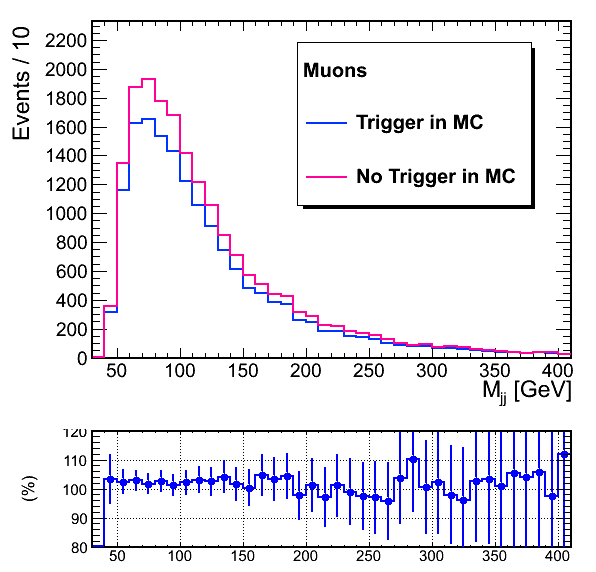
\includegraphics[width=0.48\textwidth]{figs/crosschecks/Trigger_Muons.png}
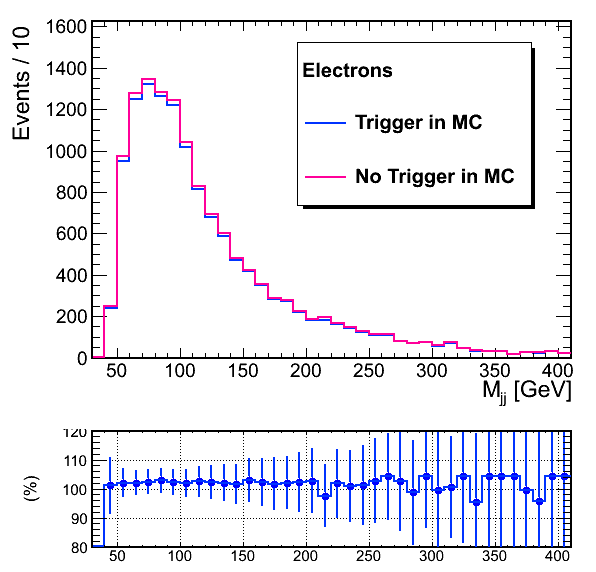
\includegraphics[width=0.48\textwidth]{figs/crosschecks/Trigger_Electrons.png}
\caption{Difference in shape for the $m_{jj}$ distribution in the W+jets 
Monte Carlo, for muons (right) and electrons (left) with and without applying 
the closest trigger paths available (chosen by an "OR" of different single 
muon or single electron paths). The lower frame shows the difference in shape, 
after correcting for the different area of both distributions.
The ratio of the two distributions is consistent with unity.} 
\label{fig:triggerEffect}}
\end{figure}
%%%%%%%
%%%%%%%%%%%%%%%%%%%%%%%%%%%%%%%%%%%%%%%
\subsection{Effect of trigger efficiency on yields}
The signal templates are corrected event-by-event for trigger 
efficiency. Since the efficiency is high (90--100\%) with weak  
dependence on lepton kinematics, the overall effect is small. 
The background yields remain unaffected by the absolute value 
of the trigger efficiency because the background yields are 
allowed to float in the fit.
%%%%%%%%%%%%%%%%%%%%%%%%%%%%%%%%%%%%%%%%%%%%%%%%%%%%%%%%%%%%%%%%%%%%
%%%%%%%%%%%%%%%%%%%%%%%%%%%%%%%%%%%%%%%%%%%%%%%%%%%%%%%%%%%%%%%%%%%%

\clearpage
\section{Study to explore the possibility to use Electron + 2 jets + missing $H_T$ trigger}
\label{sec:TriggerEpochComparison}

The trigger selection is discussed in Sections~\ref{sec:trigger}.
For electron data we initially planned to use events from 
Ele+2jet+MHT trigger. 
However, it turned out that the efficiency for jet part of 
this trigger is not well modeled for the epoch when CaloJet 
was in the trigger. We have performed a comparison of different 
epochs for ElectronHad data set, dividing
the data into two categories: one with CaloJet in the trigger and the second
with pfJet in the trigger.  
The conclusion is that
only the former has efficiency modeling problem.
We document the full study in this section. 

\subsection{Trigger epochs in ElectronHad primary dataset}
\label{sec:triggerepochsEleHad}
\begin{itemize}
\item Run2011A:Menu 5E32 (Runs: 160404--163869): \\
Ele27\_CaloIdVT\_CaloIsoT\_TrkIdT\_TrkIsoT\_v* 
\item Run2011A:Menu 1E33 (Runs: 165088--166967): \\
Ele17\_CaloIdVT\_CaloIsoT\_TrkIdT\_TrkIsoT\_CentralJet30\_CentralJet25\_PFMHT15\_v* 
\item Run2011A:Menu 1.4E33 (Runs: 167039--167913): \\
Ele22\_CaloIdVT\_CaloIsoT\_TrkIdT\_TrkIsoT\_CentralJet30\_CentralJet25\_PFMHT20\_v*
\item Run2011A:Menu 2E33 v1.1 (Runs: 170249--170759): \\
Ele22\_CaloIdVT\_CaloIsoT\_TrkIdT\_TrkIsoT\_CentralJet30\_CentralJet25\_PFMHT20\_v*
\item Run2011A:Menu 2E33 v1.2 (Runs: 170826--173198): \\
HLT\_Ele27\_CaloIdVT\_CaloIsoT\_TrkIdT\_TrkIsoT\_CentralJet30\_CentralJet25\_PFMHT20\_v*
\item Run2011A:Menu 3E33 (Runs: 173236--173692): \\
Ele27\_CaloIdVT\_CaloIsoT\_TrkIdT\_TrkIsoT\_CentralJet30\_CentralJet25\_PFMHT20\_v*
\item Run2011B: Menu 3E33 v2.0-v2.2 (Runs: 175832--178380): \\
Ele27\_CaloIdVT\_CaloIsoT\_TrkIdT\_TrkIsoT\_CentralJet30\_CentralJet25\_PFMHT20\_v2
\item Run2011B: Menu 3E33 v2.3-v5.0 (Runs: 176461--178380): \\
Ele30\_CaloIdVT\_CaloIsoT\_TrkIdT\_TrkIsoT\_DiCentralJet30\_PFMHT25\_v1
\item Run2011B: Menu 3E33 v4 (Runs: 178420--179958): \\
Ele27\_WP80\_DiCentralPFJet25\_PFMHT15\_v4
\item Run2011B: Menu 3E33 v5 (Runs: 179959--180252): \\
Ele27\_WP80\_DiCentralPFJet25\_PFMHT15\_v5
\end{itemize}
%%%%%%%%%%%%%%%%%%%%%%%%%%%%%%%%%%%%%%%%%%%%%%%%%%%%%%%%%%%
\subsection{Trigger efficiency computation for Lepton+Jet30+Jet25+MHT triggers}
\label{sec:trigeffEleHad}
The efficiency of the 
``HLT\_Ele27\_CentralJet30\_CentralJet25\_PFMHT20'' trigger 
for offline selected electron+MET+2-jet events can be computed as:
%%%%%%%%%%
\begin{equation}
\epsilon^{HLT}_{\rm{Data}} = \rm{eff(Ele27)} \times 
\rm{eff(jet1, jet2)} \times \rm{eff(MHT20)},
\end{equation}
%%%%%%%%%%
where 
%%%%%%%%%%
\begin{eqnarray}
\rm{eff(jet1, jet2)} &=& \rm{eff30(jet1)} \times \rm{eff30(jet2)} + \nonumber\\ 
                     &&\rm{eff30(jet1)} \times \rm{eff25!30(jet2)} + \nonumber\\
                     &&\rm{eff30(jet2)} \times \rm{eff25!30(jet1)}.
\end{eqnarray}
%%%%%%%%%%
If there are $N$ jets we need to systematically 
consider all combinations of  
disjoint subcases, \textit{i.e.}, whether a given jet 
\begin{itemize}
\item
passes jet30,
\item 
fails jet30 and passes jet25 (hence the nomenclature 25!30), or 
\item
fails both. 
\end{itemize}
Thus, 
%%%%%%%%%%
\begin{eqnarray}
\text{eff(jet1, ...., jetN)} &=&\text{sum over all n-jet products of efficiency outcomes,}\nonumber\\ 
                           &&\text{where any term with 2 jet30's or a jet30/jet25!30 pair}\nonumber\\ 
                           && \text{is kept, and the rest are discarded.}
\end{eqnarray}
%%%%%%%%%%
For N = 3, this leads to 27 subcases, 16 of which are kept.
Consider all 3-digit base 3 numbers and keep all of them which have a 
pair of 2's or a 1 and a 2.
Therefore, efficiency of the 
``HLT\_Ele27\_CentralJet30\_CentralJet25\_PFMHT20'' trigger 
for offline selected electron+MET+3-jet events is given by:
%%%%%%%%%%
\begin{equation}
\epsilon^{HLT}_{\rm{Data}} = \rm{eff(Ele27)} \times 
\rm{eff(jet1, jet2, jet3)} \times \rm{eff(MHT20)},
\end{equation}
%%%%%%%%%%
where 
%%%%%%%%%%
\begin{eqnarray}
\rm{eff(jet1, jet2, jet3)} &=&  
[1-\rm{eff30(jet1)}- \rm{eff25!30(jet1)}] \cdot \rm{eff25!30(jet2)} \cdot \rm{eff30(jet3)} \,\,\,
\rm{\textcolor{red}{(\textit{i.e.}, term "012")}} \nonumber\\
  && +``021'' + ``022'' + ``102'' + ``112'' + ``120'' + ``121'' + ``122'' +``201'' \nonumber\\
  && + ``202'' + ``210'' + ``211'' + ``212'' + ``220'' + ``221'' + ``222''.
\end{eqnarray}
%%%%%%%%%%
The N jet generalization is as follows.  
Consider all N-digit base-3 numbers\\

for i[1] = 0 to 2 \\
for i[2] = 0 to 2 \\
...\\
for i[N] = 0 to 2\\

if {i[1], ..., i[N] } has a pair of 2's or a 1 and a 2\\
    effN += effi[1] * effi[2] * ... effi[N],\\

where each effi is either eff30, eff25!30, or 1 $-$ eff30 $-$ eff25!30.
%%%%%%%%%%%%%%%%%%%%%%%%%%%%%%%%%%%%%%%%%%%%%%%%%%%%%%%%%%%
\subsection{Lepton+Jet30+Jet30+MHT triggers}
%%%%%%%%%%%%%%%%%%%%%%%%%%%%%%%%%%%%%%%%%%%%%%%%%%%%%%%%%%%
The efficiency of the 
``HLT\_Ele30\_DiCentralJet30\_PFMHT25'' trigger 
for offline selected electron+MET+2-jet events can be computed as:
%%%%%%%%%%
\begin{equation}
\epsilon^{HLT}_{\rm{Data}} = \rm{eff(Ele30)} \times 
\rm{eff(jet1, jet2)} \times \rm{eff(MHT25)},
\end{equation}
%%%%%%%%%%
where 
%%%%%%%%%%
\begin{equation}
\rm{eff(jet1, jet2)} = \rm{eff30(jet1)} \times \rm{eff30(jet2)}. 
\end{equation}
%%%%%%%%%%

The efficiency of the 
``HLT\_Ele30\_DiCentralJet30\_PFMHT25'' trigger 
for offline selected electron+MET+3-jet events can be computed as:
%%%%%%%%%%
\begin{equation}
\epsilon^{HLT}_{\rm{Data}} = \rm{eff(Ele30)} \times 
\rm{eff(jet1, jet2, jet3)} \times \rm{eff(MHT25)},
\end{equation}
%%%%%%%%%%
where 
%%%%%%%%%%
\begin{eqnarray}
\rm{eff(jet1, jet2, jet3)} &=& 
[1-\rm{eff30(jet1)}] \cdot \rm{eff30(jet2)} \cdot \rm{eff30(jet3)} +\nonumber\\
&&\rm{eff30(jet1)} \cdot [1-\rm{eff30(jet2)}] \cdot \rm{eff30(jet3)} +\nonumber\\
&&\rm{eff30(jet1)} \cdot \rm{eff30(jet2)} \cdot [1-\rm{eff30(jet3)}] + \nonumber\\
&&\rm{eff30(jet1)} \cdot \rm{eff30(jet2)} \cdot \rm{eff30(jet3)}.
\end{eqnarray}
%%%%%%%%%%
%%%%%%%%%%%
\subsection{Electron+2Jet+MHT trigger efficiency table: Electron leg}
\label{sec:trigeff_HLTEle2jPfMht_ele}
The luminosity weighted average trigger efficiency 
for electron leg of the Electron+2Jet+MHT triggers in data is given 
in Table~\ref{tab:eleEff_HLTEle2jPfMht_ele}.
%%%%%%%%%%%
%\verbatiminput{eleEffsHLTEle2jPfMht_data_LWA_Ele.txt}
%%%%%%%%%%%%%%%%%%%%%%%%%%%%%
\begin{table}[bthp]
\begin{center}
  \begin{tabular}{l l c | l c}
    \hline  \hline
    $p_T$ range (GeV) & $\eta$ range  & $\epsilon_{\rm{Data}}$ & 
    $\eta$ range  & $\epsilon_{\rm{Data}}$\\
    \hline  
    30--35 &	-2.5-- -1.5 & 0.8742 $\pm$ 0.0039 & 1.5--2.5 & 0.8519 $\pm$ 0.0040 \\
           &	-1.5-- 0.0  & 0.9711 $\pm$ 0.0010 & 0.0--1.5 & 0.9690 $\pm$ 0.0011 \\
    \hline  
    35--40 &	-2.5-- -1.5 & 0.9630 $\pm$ 0.0017 & 1.5--2.5 & 0.9623 $\pm$ 0.0017 \\
           &	-1.5-- 0.0  & 0.9775 $\pm$ 0.0006 & 0.0--1.5 & 0.9757 $\pm$ 0.0007 \\
    \hline  
    40--45 &	-2.5-- -1.5 & 0.9720 $\pm$ 0.0013 & 1.5--2.5 & 0.9699 $\pm$ 0.0013 \\
           &	-1.5-- 0.0  & 0.9789 $\pm$ 0.0006 & 0.0--1.5 & 0.9762 $\pm$ 0.0006 \\
    \hline 
    45--50 &	-2.5-- -1.5 & 0.9720 $\pm$ 0.0014 & 1.5--2.5 & 0.9727 $\pm$ 0.0014 \\
           &	-1.5-- 0.0  & 0.9782 $\pm$ 0.0007 & 0.0--1.5 & 0.9764 $\pm$ 0.0007 \\
    \hline  
    50--200&	-2.5-- -1.5 & 0.9747 $\pm$ 0.0017 & 1.5--2.5 & 0.9746 $\pm$ 0.0016 \\
           &	-1.5-- 0.0  & 0.9820 $\pm$ 0.0008 & 0.0--1.5 & 0.9808 $\pm$ 0.0008 \\
    \hline  \hline
  \end{tabular}
\end{center}
\caption{\label{tab:eleEff_HLTEle2jPfMht_ele}
Trigger efficiency in data for the electron portion of the
HLTEle2jPfMht trigger (LWA for Lepton-Photon dataset).  The uncertainties are
statistical only.}
\end{table}
%%%%%%%%%%%
\subsection{Electron+2Jet+MHT trigger efficiency table: Jet30}
\label{sec:trigeff_HLTEle2jPfMht_jet30}
The luminosity weighted average trigger efficiency 
for the Jet30 leg of the Electron+2Jet+MHT triggers in data is given 
in Table~\ref{tab:eleEff_HLTEle2jPfMht_jet30}. There is a slow turn-on exhibited,
and the trigger efficiency is constant only for jet $p_T > 50$~GeV.
%%%%%%%%%%%
%\verbatiminput{eleEffsHLTEle2jPfMht_data_LWA_Jet30.txt}
\begin{table}[bthp]
\begin{center}
  \begin{tabular}{l l c | l c}
    \hline  \hline
    $p_T$ range (GeV) & $\eta$ range  & $\epsilon_{\rm{Data}}$ & 
    $\eta$ range  & $\epsilon_{\rm{Data}}$\\
    \hline  
    30--35 &	-2.4-- -1.5 & 0.4209 $\pm$ 0.0092 & 1.5--2.4 & 0.4292 $\pm$ 0.0090 \\
           &	-1.5-- 0.0  & 0.5051 $\pm$ 0.0064 & 0.0--1.5 & 0.5051 $\pm$ 0.0064 \\
    \hline  
    35--40 &	-2.4-- -1.5 & 0.7081 $\pm$ 0.0100 & 1.5--2.4 & 0.6849 $\pm$ 0.0100 \\
           &	-1.5-- 0.0  & 0.7268 $\pm$ 0.0062 & 0.0--1.5 & 0.7109 $\pm$ 0.0063 \\
    \hline  
    40--45 &	-2.4-- -1.5 & 0.8689 $\pm$ 0.0090 & 1.5--2.4 & 0.8630 $\pm$ 0.0088 \\
           &	-1.5-- 0.0  & 0.8562 $\pm$ 0.0057 & 0.0--1.5 & 0.8693 $\pm$ 0.0054 \\
    \hline  
    45--50 &	-2.4-- -1.5 & 0.9522 $\pm$ 0.0067 & 1.5--2.4 & 0.9377 $\pm$ 0.0077 \\
           &	-1.5-- 0.0  & 0.9343 $\pm$ 0.0047 & 0.0--1.5 & 0.9318 $\pm$ 0.0047 \\
    \hline  
    50--55 &	-2.4-- -1.5 & 0.9698 $\pm$ 0.0064 & 1.5--2.4 & 0.9751 $\pm$ 0.0058 \\
           &	-1.5-- 0.0  & 0.9734 $\pm$ 0.0035 & 0.0--1.5 & 0.9622 $\pm$ 0.0041 \\
    \hline  
    55--60 &	-2.4-- -1.5 & 0.9847 $\pm$ 0.0055 & 1.5--2.4 & 0.9743 $\pm$ 0.0066 \\
           &	-1.5-- 0.0  & 0.9800 $\pm$ 0.0034 & 0.0--1.5 & 0.9802 $\pm$ 0.0035 \\
    \hline  
    60--65 &	-2.4-- -1.5 & 0.9767 $\pm$ 0.0076 & 1.5--2.4 & 0.9807 $\pm$ 0.0066 \\
           &	-1.5-- 0.0  & 0.9884 $\pm$ 0.0030 & 0.0--1.5 & 0.9871 $\pm$ 0.0033 \\
    \hline  
    65--70 &	-2.4-- -1.5 & 0.9829 $\pm$ 0.0071 & 1.5--2.4 & 0.9891 $\pm$ 0.0064 \\
           &	-1.5-- 0.0  & 0.9904 $\pm$ 0.0032 & 0.0--1.5 & 0.9861 $\pm$ 0.0036 \\
    \hline  
    70--80 &	-2.4-- -1.5 & 0.9915 $\pm$ 0.0044 & 1.5--2.4 & 0.9904 $\pm$ 0.0046 \\
           &	-1.5-- 0.0  & 0.9893 $\pm$ 0.0025 & 0.0--1.5 & 0.9904 $\pm$ 0.0024 \\
    \hline  
    80--90 &	-2.4-- -1.5 & 0.9915 $\pm$ 0.0056 & 1.5--2.4 & 0.9963 $\pm$ 0.0047 \\
           &	-1.5-- 0.0  & 0.9914 $\pm$ 0.0027 & 0.0--1.5 & 0.9915 $\pm$ 0.0027 \\
    \hline  
    90--100 &	-2.4-- -1.5 & 0.9897 $\pm$ 0.0074 & 1.5--2.4 & 0.9924 $\pm$ 0.0060 \\
           &	-1.5-- 0.0  & 0.9912 $\pm$ 0.0033 & 0.0--1.5 & 0.9909 $\pm$ 0.0032 \\
    \hline  
    100--200&	-2.4-- -1.5 & 0.9924 $\pm$ 0.0032 & 1.5--2.4 & 0.9925 $\pm$ 0.0032 \\
           &	-1.5-- 0.0  & 0.9951 $\pm$ 0.0013 & 0.0--1.5 & 0.9953 $\pm$ 0.0012 \\
    \hline  \hline
  \end{tabular}
\end{center}
\caption{\label{tab:eleEff_HLTEle2jPfMht_jet30}
Trigger efficiency in data for jet30 portion of HLTEle2jPfMht (LWA for Lepton-Photon dataset). 
The uncertainties are statistical only.}
\end{table}
%%%%%%%%%%%%%%%%%%%%%%%%%%%%%%%%%%%%%%%%%%%%%%%%%%%%%%%%%%%%%%%%%%%%
%%%%%%%%%%%
\subsection{Electron+2Jet+MHT trigger efficiency table: Jet25!30}
\label{sec:trigeff_HLTEle2jPfMht_jet25not30}
The luminosity weighted average trigger efficiency for the Jet25!30
leg ($25 < \rm{online jet~}p_T < 30$~GeV) of the Electron+2Jet+MHT
triggers in data is given in
Table~\ref{tab:eleEff_HLTEle2jPfMht_jet25not30}. This is calculated
for offline jet $p_T$s in excess of 30~GeV. A non-negligible
contribution is expected from this leg due to the steeply falling jet
$p_T$ distribution combined with poor jet resolution
online and the change in jet reconstruction algorithms from online to
offline.
%%%%%%%%%%%
%\verbatiminput{eleEffsHLTEle2jPfMht_data_LWA_Jet25Not30.txt}
\begin{table}[bthp]
\begin{center}
  \begin{tabular}{l l c | l c}
    \hline  \hline
    $p_T$ range (GeV) & $\eta$ range  & $\epsilon_{\rm{Data}}$ & 
    $\eta$ range  & $\epsilon_{\rm{Data}}$\\
    \hline  
    30--35 &	-2.4-- -1.5 & 0.1923 $\pm$ 0.0070 & 1.5--2.4 & 0.2124 $\pm$ 0.0071 \\
           &	-1.5-- 0.0  & 0.1468 $\pm$ 0.0043 & 0.0--1.5 & 0.1516 $\pm$ 0.0043 \\
    \hline 
    35--40 &	-2.4-- -1.5 & 0.0892 $\pm$ 0.0055 & 1.5--2.4 & 0.1168 $\pm$ 0.0061 \\
           &	-1.5-- 0.0  & 0.0792 $\pm$ 0.0033 & 0.0--1.5 & 0.0885 $\pm$ 0.0034 \\
    \hline 
    40--45 &	-2.4-- -1.5 & 0.0374 $\pm$ 0.0041 & 1.5--2.4 & 0.0368 $\pm$ 0.0041 \\
           &	-1.5-- 0.0  & 0.0337 $\pm$ 0.0024 & 0.0--1.5 & 0.0378 $\pm$ 0.0025 \\
    \hline  
    45--50 &	-2.4-- -1.5 & 0.0154 $\pm$ 0.0031 & 1.5--2.4 & 0.0212 $\pm$ 0.0035 \\
           &	-1.5-- 0.0  & 0.0139 $\pm$ 0.0018 & 0.0--1.5 & 0.0146 $\pm$ 0.0018 \\
    \hline
    50--55 &	-2.4-- -1.5 & 0.0061 $\pm$ 0.0024 & 1.5--2.4 & 0.0053 $\pm$ 0.0022 \\
           &	-1.5-- 0.0  & 0.0051 $\pm$ 0.0012 & 0.0--1.5 & 0.0076 $\pm$ 0.0015 \\
    \hline  
    55--60 &	-2.4-- -1.5 & 0.0027 $\pm$ 0.0021 & 1.5--2.4 & 0.0028 $\pm$ 0.0019 \\
           &	-1.5-- 0.0  & 0.0020 $\pm$ 0.0009 & 0.0--1.5 & 0.0041 $\pm$ 0.0013 \\
    \hline  
    60--65 &	-2.4-- -1.5 & 0.0016 $\pm$ 0.0020 & 1.5--2.4 & 0.0006 $\pm$ 0.0016 \\
           &	-1.5-- 0.0  & 0.0018 $\pm$ 0.0010 & 0.0--1.5 & 0.0014 $\pm$ 0.0010 \\
    \hline  
    65--70 &	-2.4-- -1.5 & 0.0008 $\pm$ 0.0020 & 1.5--2.4 & 0.0000 $\pm$ 0.0017 \\
           &	-1.5-- 0.0  & 0.0010 $\pm$ 0.0009 & 0.0--1.5 & 0.0000 $\pm$ 0.0006 \\
    \hline  
    70--80 &	-2.4-- -1.5 & 0.0005 $\pm$ 0.0012 & 1.5--2.4 & 0.0000 $\pm$ 0.0011 \\
           &	-1.5-- 0.0  & 0.0004 $\pm$ 0.0005 & 0.0--1.5 & 0.0004 $\pm$ 0.0005 \\
    \hline  
    80--90 &	-2.4-- -1.5 & 0.0000 $\pm$ 0.0016 & 1.5--2.4 & 0.0007 $\pm$ 0.0017 \\
           &	-1.5-- 0.0  & 0.0003 $\pm$ 0.0006 & 0.0--1.5 & 0.0006 $\pm$ 0.0007 \\
    \hline  
    90--100 &	-2.4-- -1.5 & 0.0000 $\pm$ 0.0020 & 1.5--2.4 & 0.0000 $\pm$ 0.0019 \\
           &	-1.5-- 0.0  & 0.0004 $\pm$ 0.0008 & 0.0--1.5 & 0.0000 $\pm$ 0.0006 \\
    \hline 
    100--200&	-2.4-- -1.5 & 0.0000 $\pm$ 0.0007 & 1.5--2.4 & 0.0000 $\pm$ 0.0007 \\
           &	-1.5-- 0.0  & 0.0001 $\pm$ 0.0003 & 0.0--1.5 & 0.0001 $\pm$ 0.0003 \\
    \hline  \hline
  \end{tabular}
\end{center}
\caption{\label{tab:eleEff_HLTEle2jPfMht_jet25not30}
Trigger efficiency in data for the ``jet25 AND NOT jet30'' portion of
the HLTEle2jPfMht trigger (LWA for Lepton-Photon dataset); i.e., for
jets passing the jet25 trigger but not the jet30 trigger.  The
uncertainties are statistical only.}
\end{table}
%%%%%%%%%%%%%%%%%%%%%%%%%%%%%%%%%%%%%%%%%%%%%%%%%%%%%%%%%%%%%%%%%%%%
%%%%%%%%%%%
\subsection{Electron+2Jet+MHT trigger efficiency table: MHT}
\label{sec:trigeff_HLTEle2jPfMht_pfmht}
The luminosity weighted average trigger efficiency 
for the MHT leg of the Electron+2Jet+MHT triggers in data is given 
in Table~\ref{tab:eleEff_HLTEle2jPfMht_pfmht}. Note that the trigger for MHT is
reasonably constant only for MHT values greater than about 40~GeV.
%%%%%%%%%%%
%\verbatiminput{eleEffsHLTEle2jPfMht_data_LWA_PfMht.txt}
%%%%%%%%%%%%%%%%%%%%%%%%%%%%%
\begin{table}[bthp]
\begin{center}
  \begin{tabular}{l c}
    \hline  \hline
    Offline missing $E_T$ (GeV) & $\epsilon_{\rm{Data}}$ \\
    \hline  
    30--35  &	0.9136   $\pm$	0.0072 \\
    35--40  &	0.9393   $\pm$	0.0064 \\
    40--45  &	0.9807   $\pm$	0.0045 \\
    45--50  &	0.9821   $\pm$	0.0055 \\
    50--60  &	0.9933   $\pm$	0.0030 \\
    60--70  &	0.9955   $\pm$	0.0049 \\
    70--100 &	0.9954   $\pm$	0.0037 \\
    100--500 &	1.0   $\pm$	0.0 \\
    \hline  \hline
  \end{tabular}
\end{center}
\caption{\label{tab:eleEff_HLTEle2jPfMht_pfmht}
Trigger efficiency in data for the PF MHT portion of the HLTEle2jPfMht 
trigger (LWA for Lepton-Photon dataset). 
The uncertainties are statistical only.}
\end{table}
%%%%%%%%%%%%%%%%%%%%%%%%%%%%%%%%%%%%%%%
%%%%%%%%%%%%%%%%%%%%%%%%%%%%%%%%%%%%%%%
\clearpage
\subsection{Effect of trigger efficiency on shapes}
%%%%%%%%%%%%%%%%%%%%
\begin{figure}[h!t]
  {\centering
  \subfigure[]{
  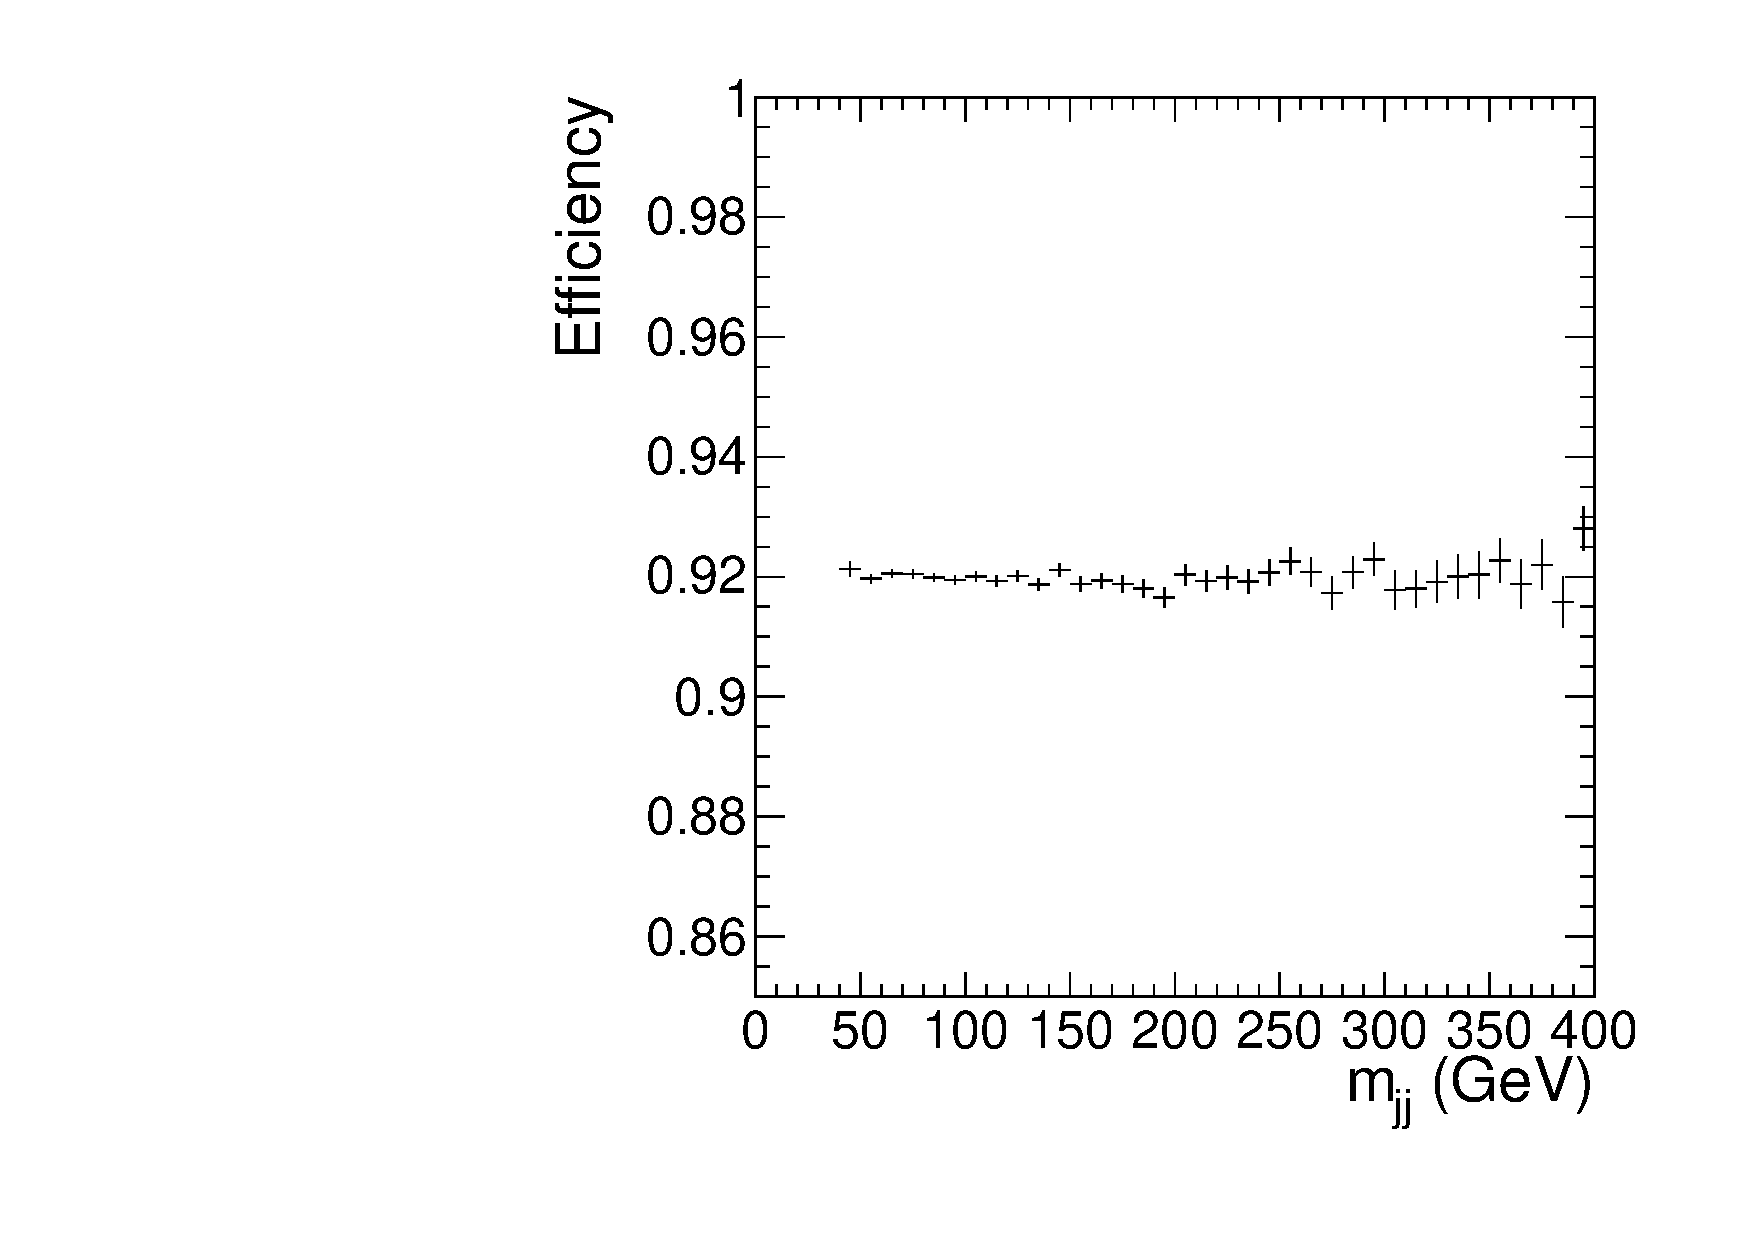
\includegraphics[width=0.4\textwidth]{figs/effPlots/fig_eff_HLTEle2jPfMht_ele.pdf}
  }   
  \subfigure[]{
  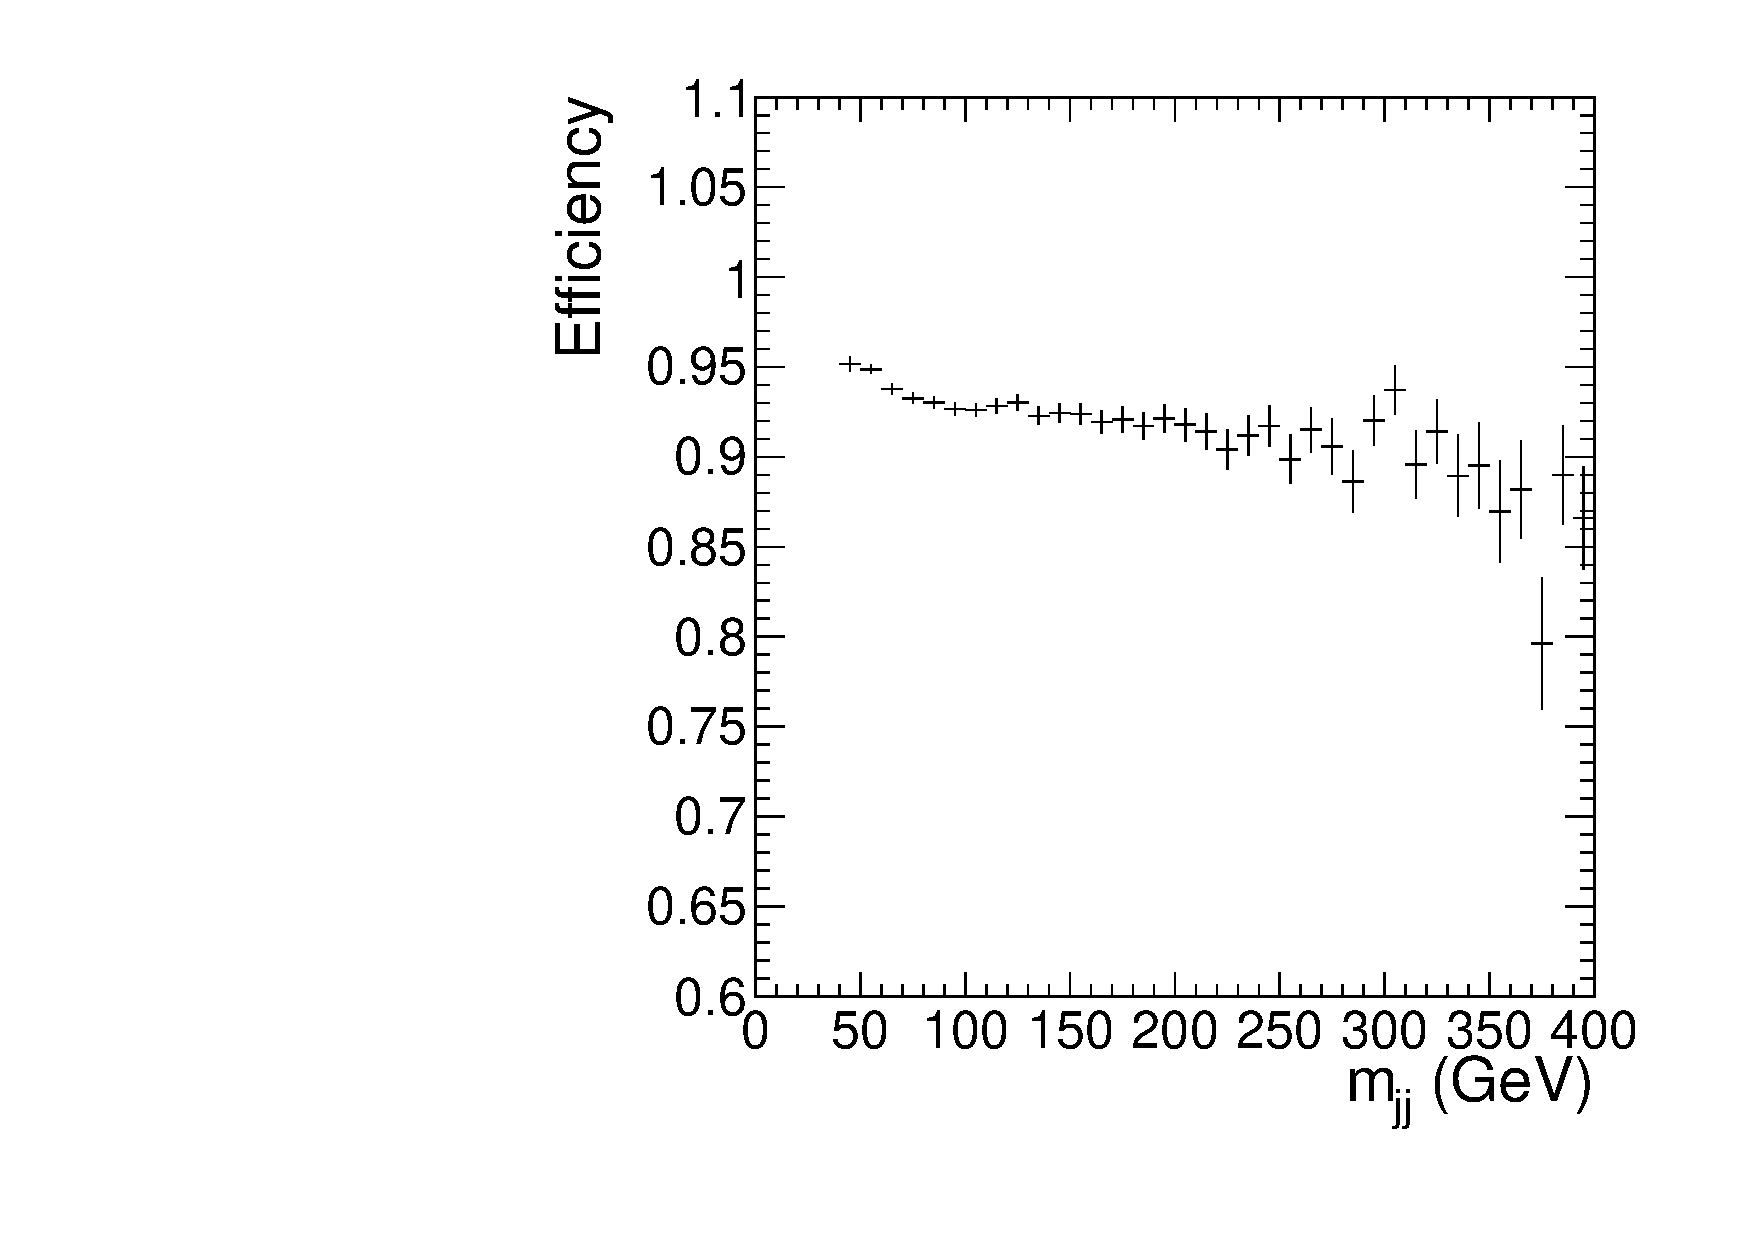
\includegraphics[width=0.4\textwidth]{figs/effPlots/fig_eff_HLTEle2jPfMht_mht.pdf}
   }
   \vspace*{1mm} \\
   \subfigure[]{
   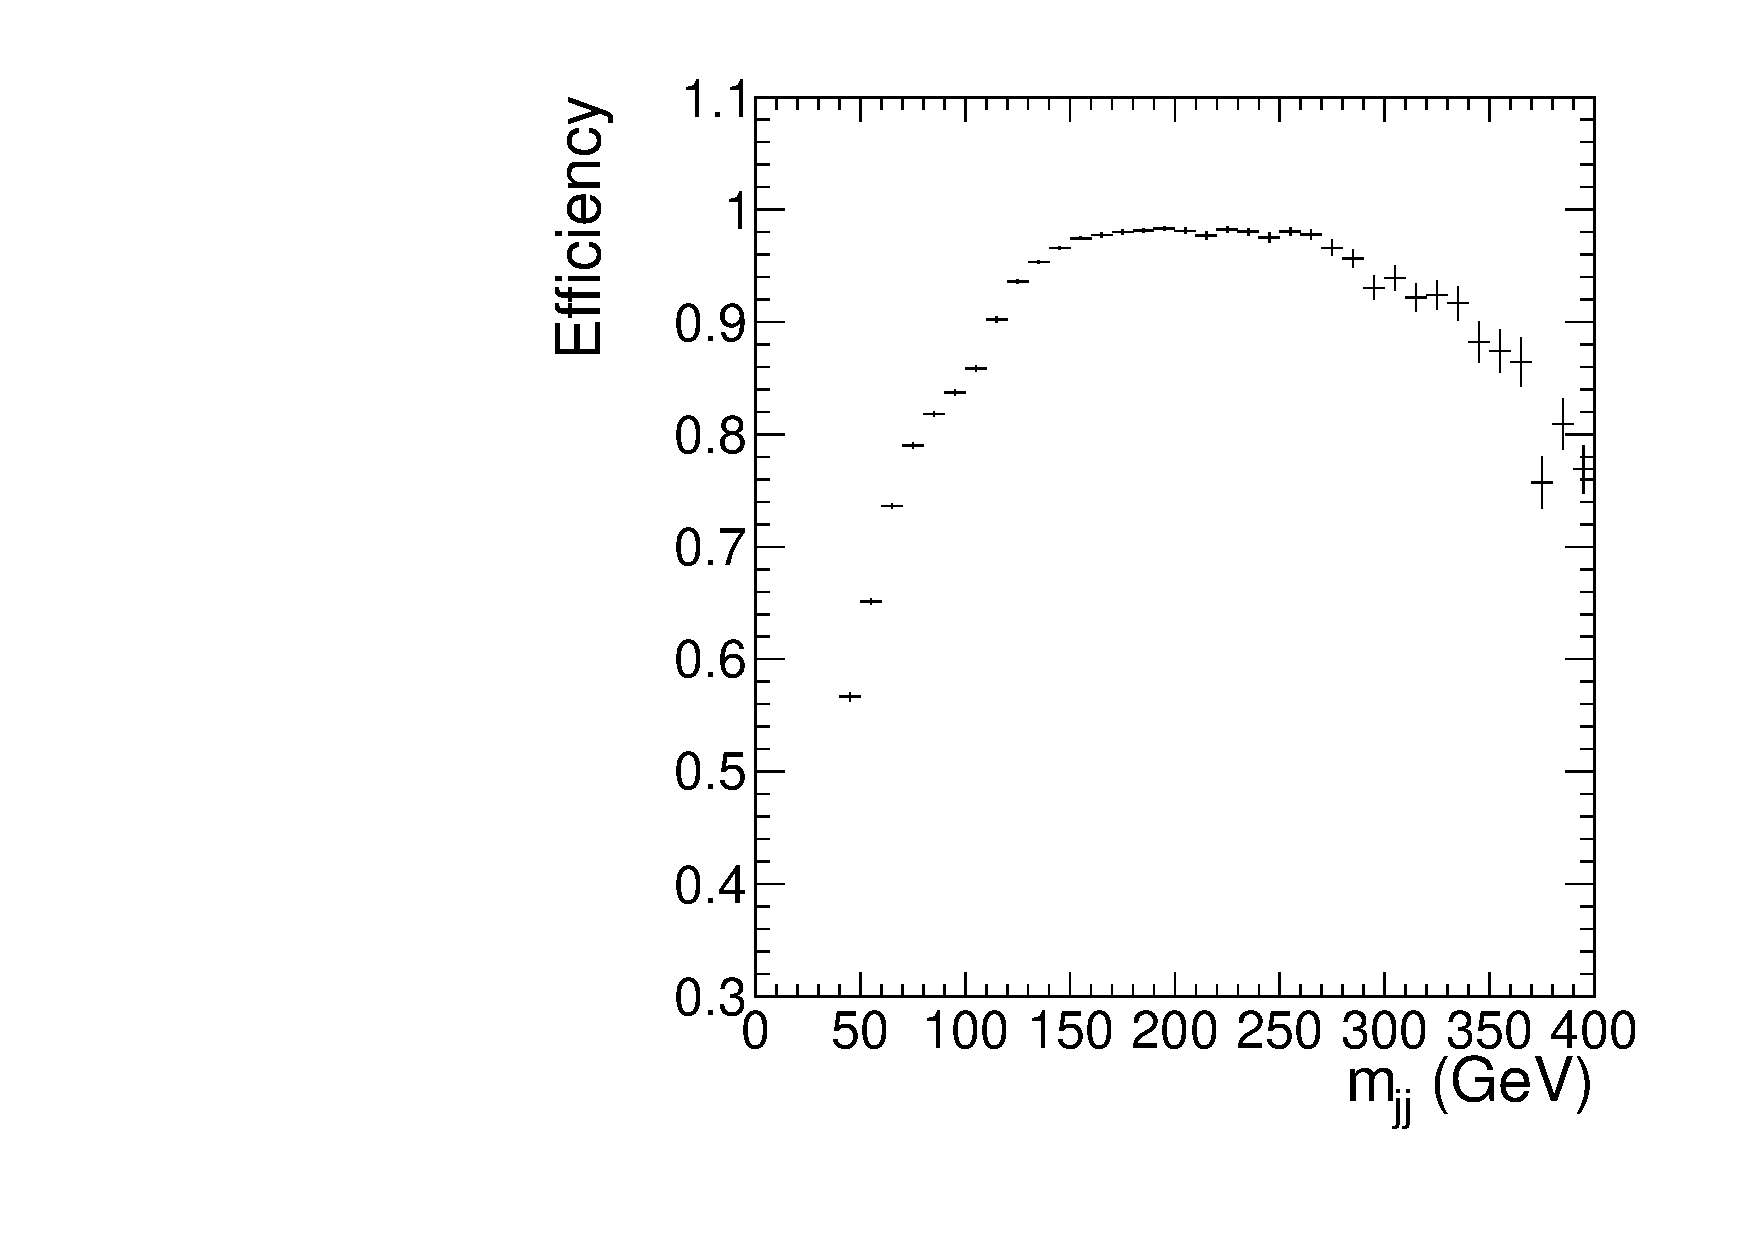
\includegraphics[width=0.4\textwidth]{figs/effPlots/fig_eff_HLTEle2jPfMht_dijet.pdf}
   }
   \subfigure[]{
   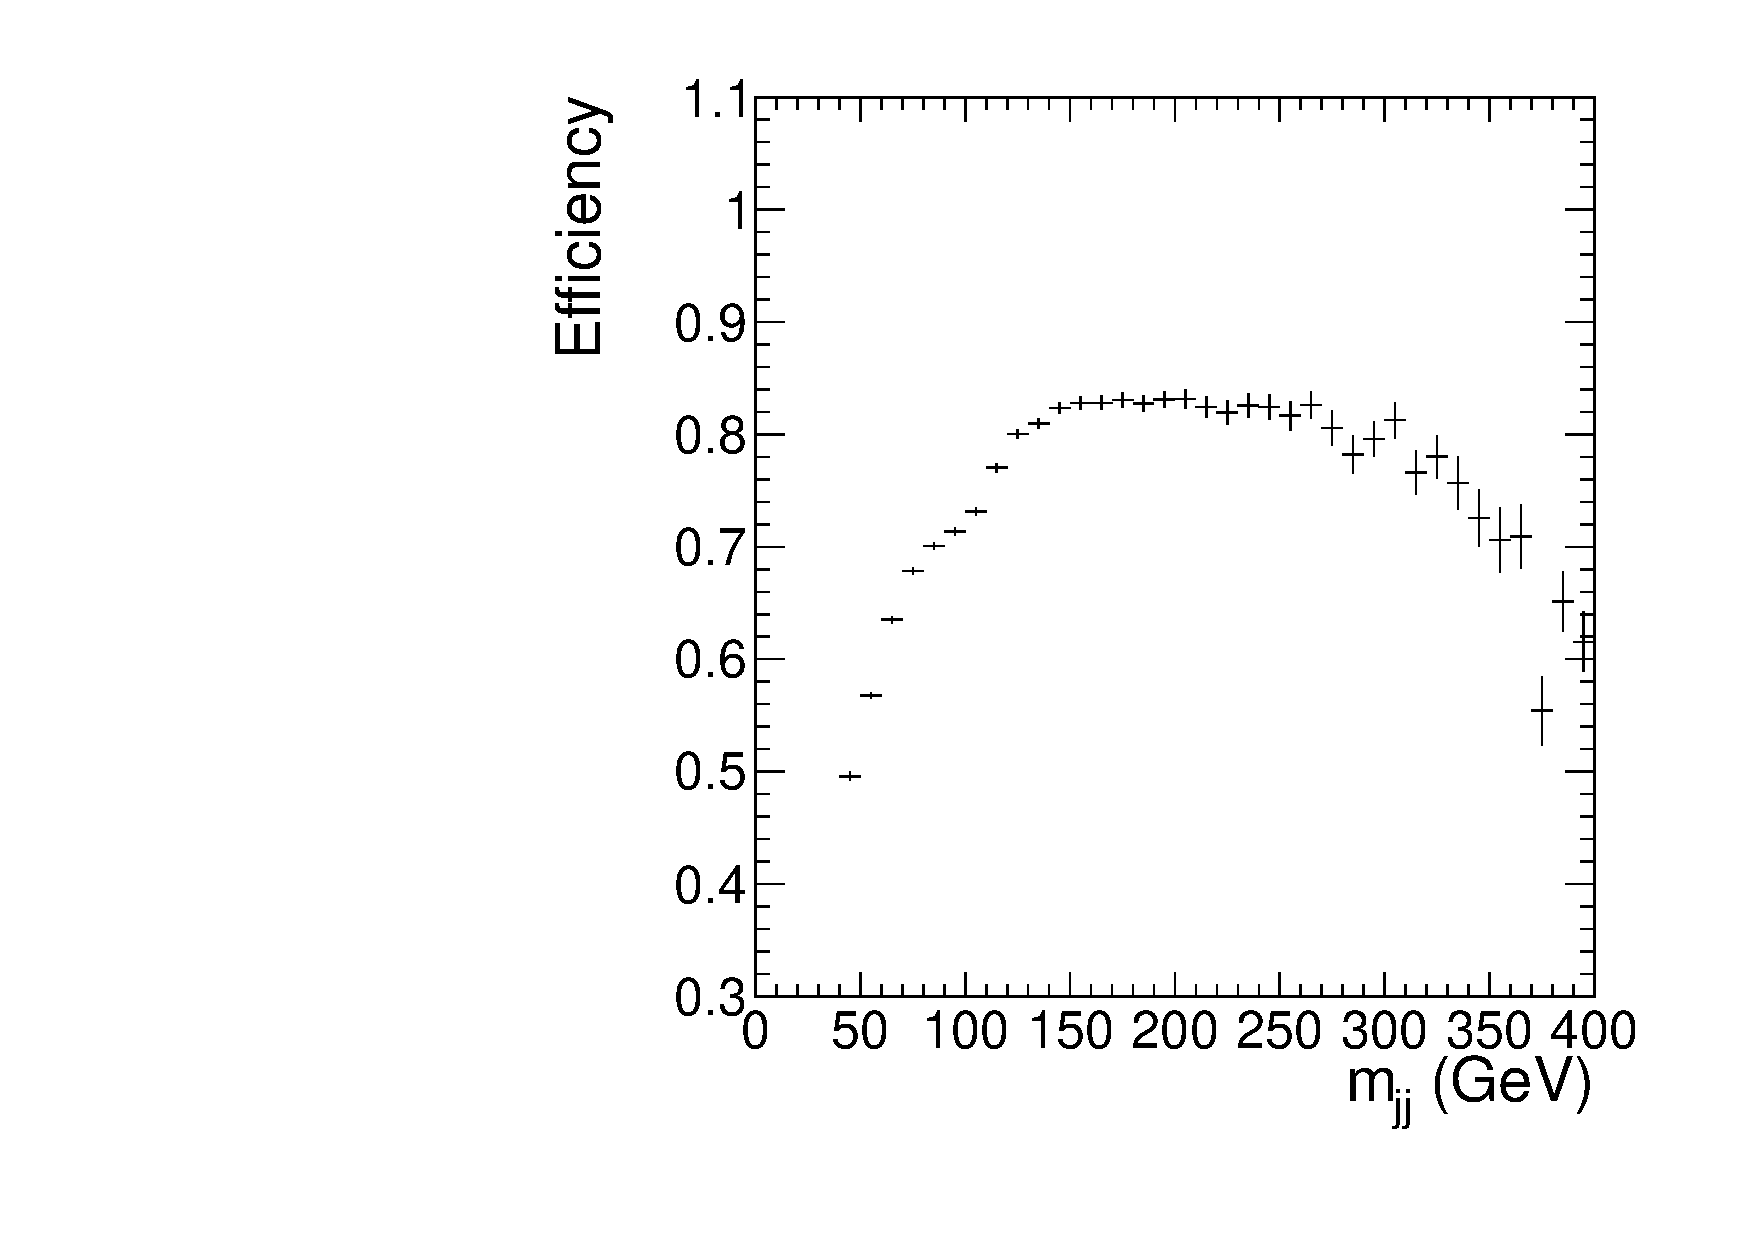
\includegraphics[width=0.4\textwidth]{figs/effPlots/fig_eff_HLTEle2jPfMht_total.pdf}
   }
   \vspace*{1mm} \\
   \subfigure[]{
   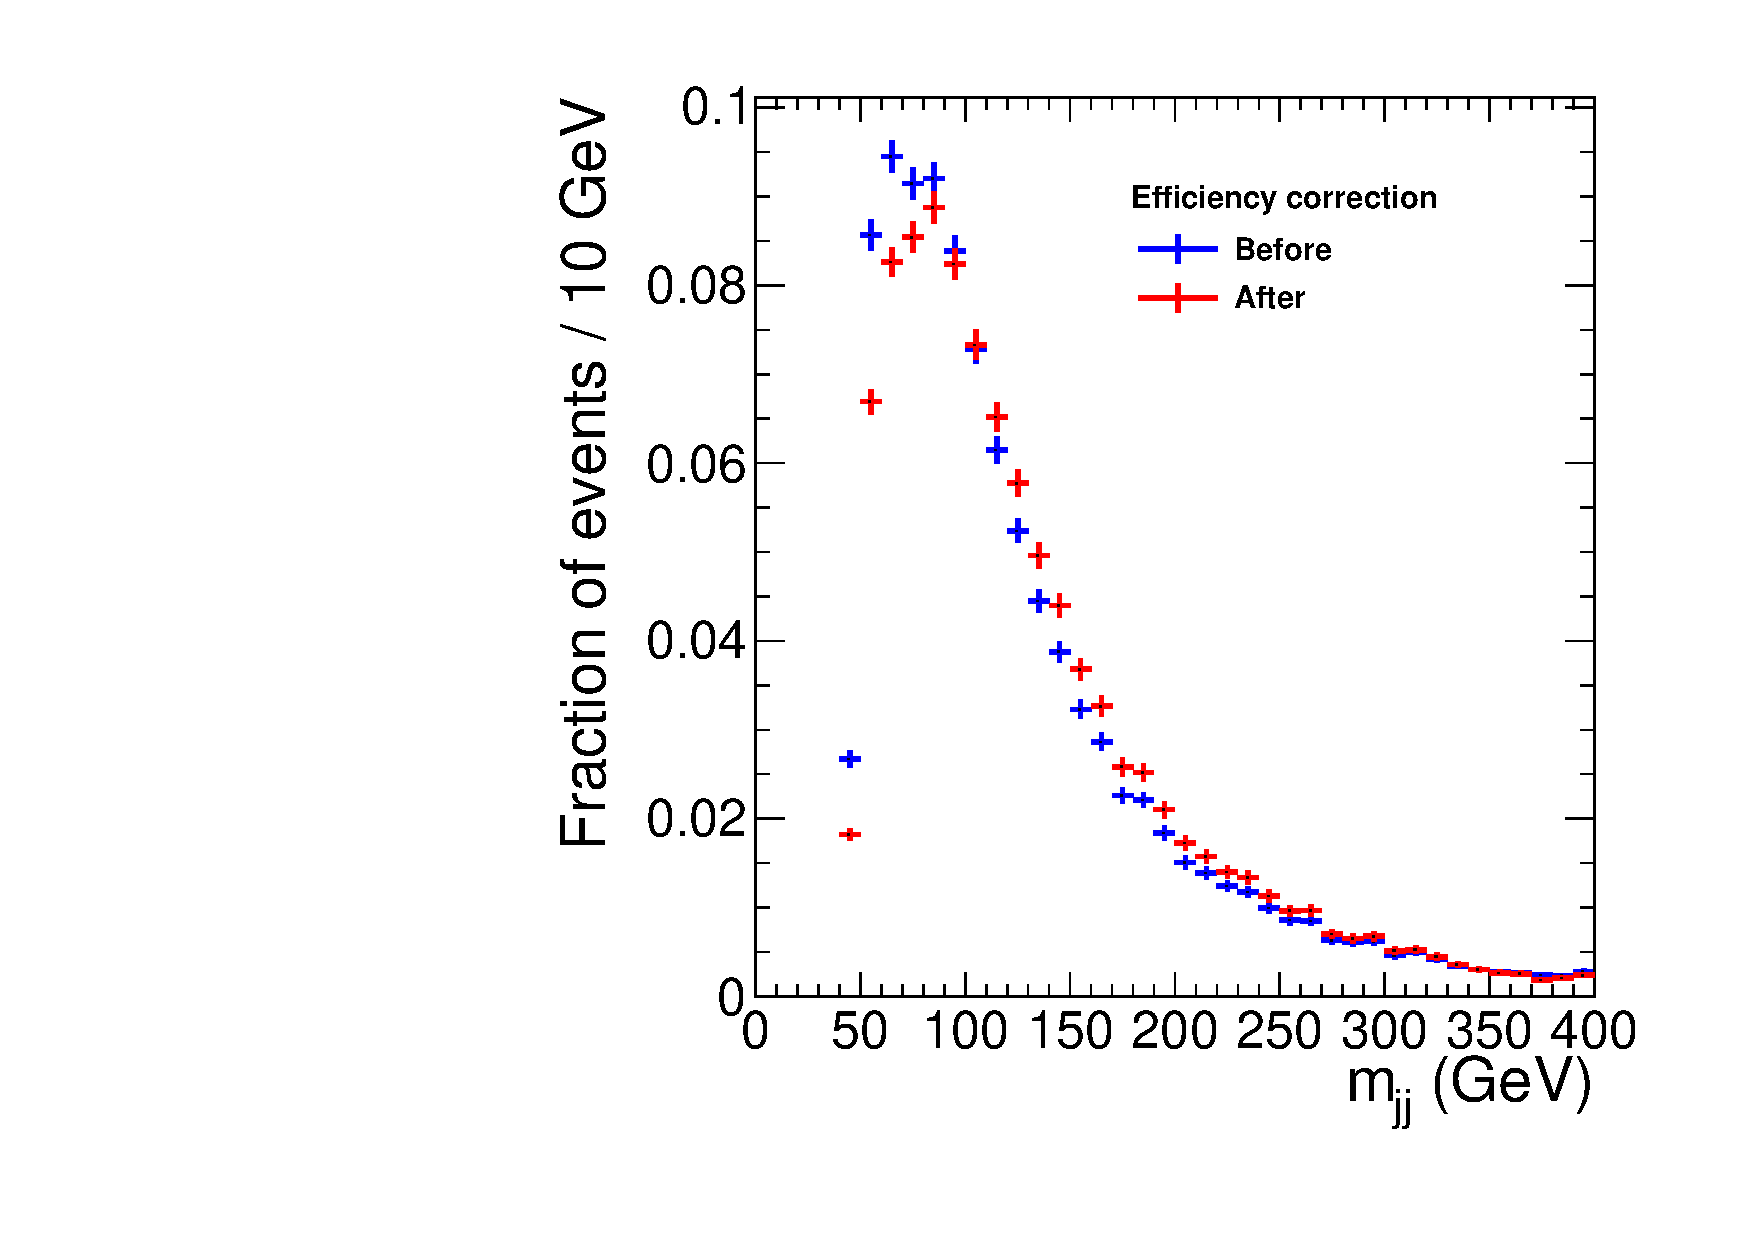
\includegraphics[width=0.4\textwidth]{figs/effPlots/fig_eff_HLTEle2jPfMht_template.pdf}
   }
   \subfigure[]{
   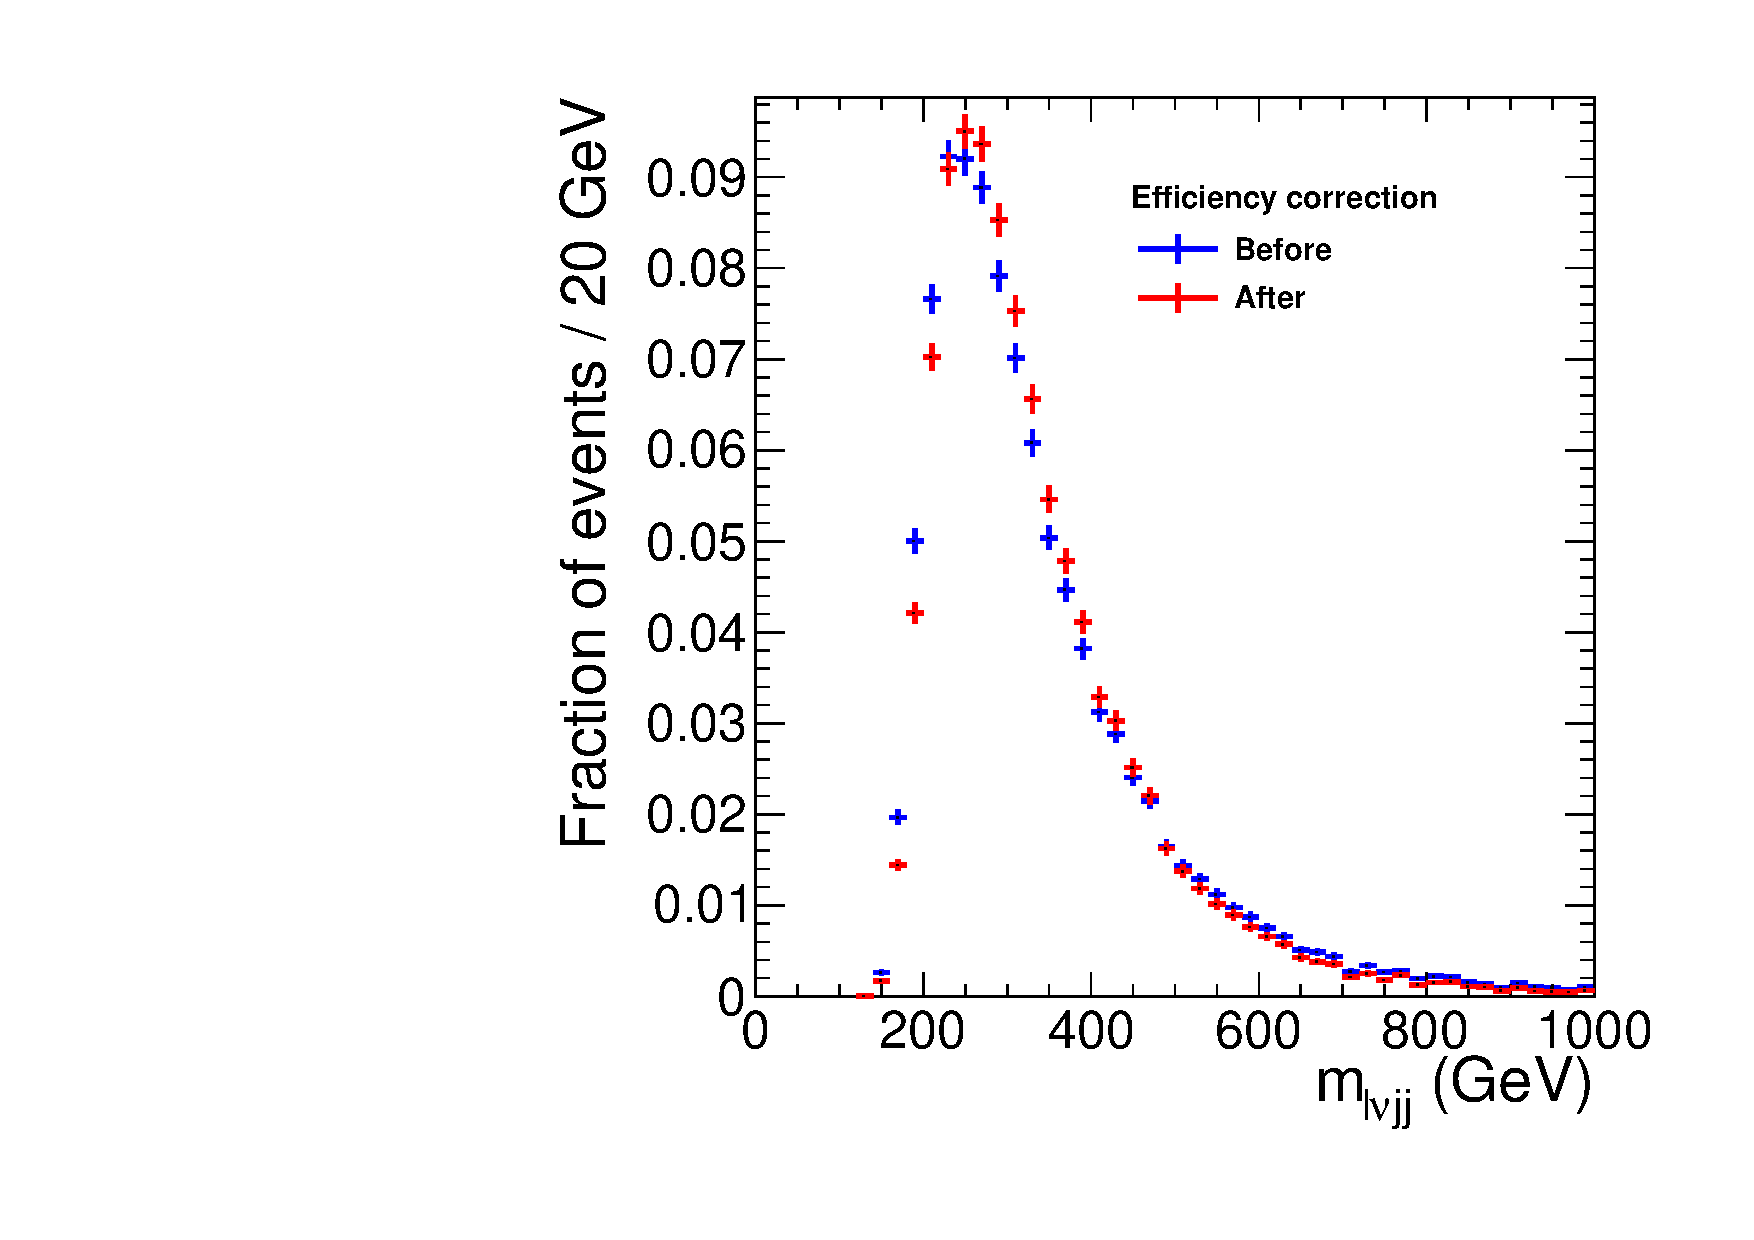
\includegraphics[width=0.4\textwidth]{figs/effPlots/fig_eff_HLTEle2jPfMht_template4body.pdf}
   }
   \caption{For W+jets background: Luminosity weighted average trigger efficiency in the 
   electron + 2jet + missing $H_T$ trigger as a function of $m_{jj}$: (a) for the electrong leg, 
   (b) for the missing $H_T$ leg, (c) for the dijet leg, and (d) total, \textit{i.e.}, the product 
   of the efficiencies for the three legs. 
   The effect of this efficiency correction on W+jets shape is shown for 
   $m_{jj}$ (e) and $m_{\ell\nu jj}$ (f) templates.}
\label{fig:EleHadhlteff}}
\end{figure}
%%%%%%%%%%%%%%%%%%%%
%%%%%%%%%%%%%%%%%%%%
%%%%%%%%%%%%%%%%%%%%
\begin{figure}[h!t]
  {\centering
  \subfigure[]{
  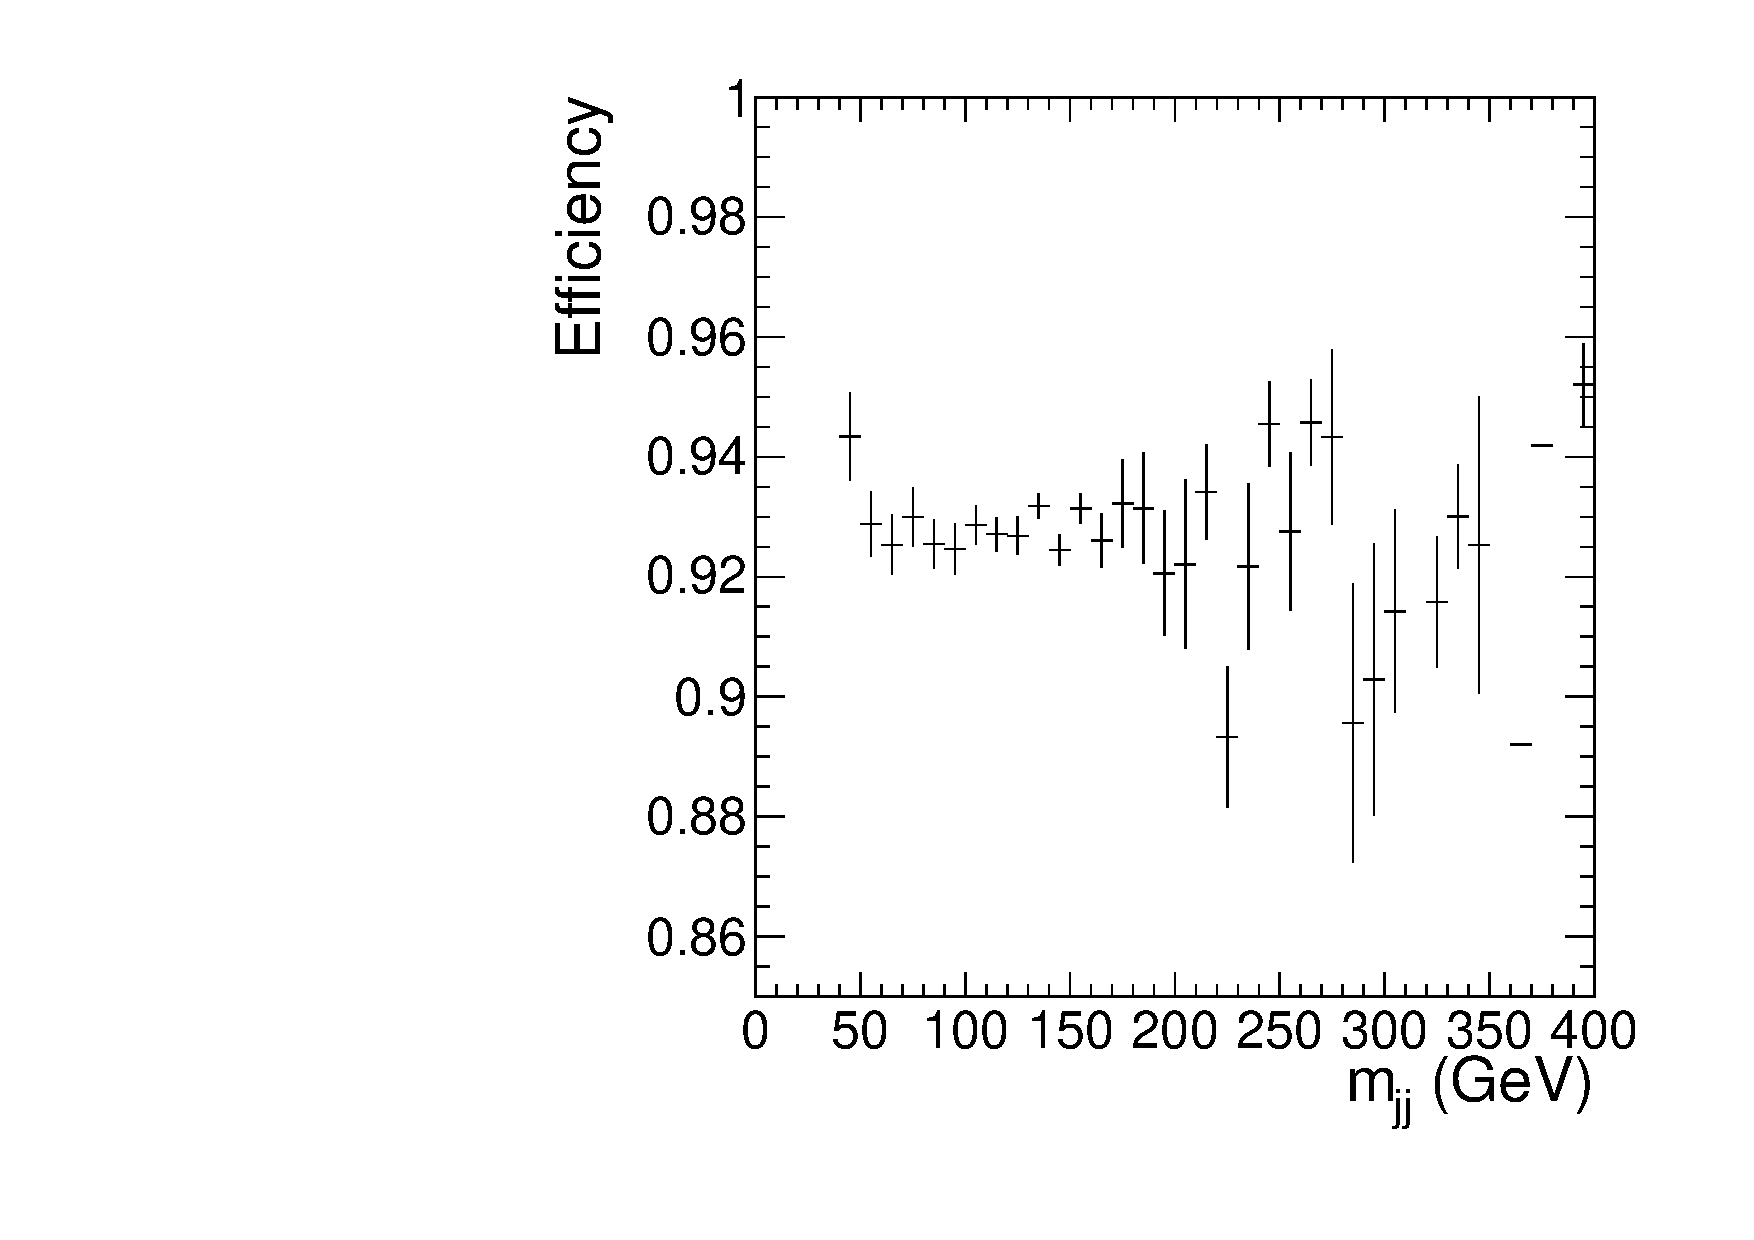
\includegraphics[width=0.4\textwidth]{figs/effPlots/fig_WH_eff_HLTEle2jPfMht_ele.pdf}
  }   
  \subfigure[]{
  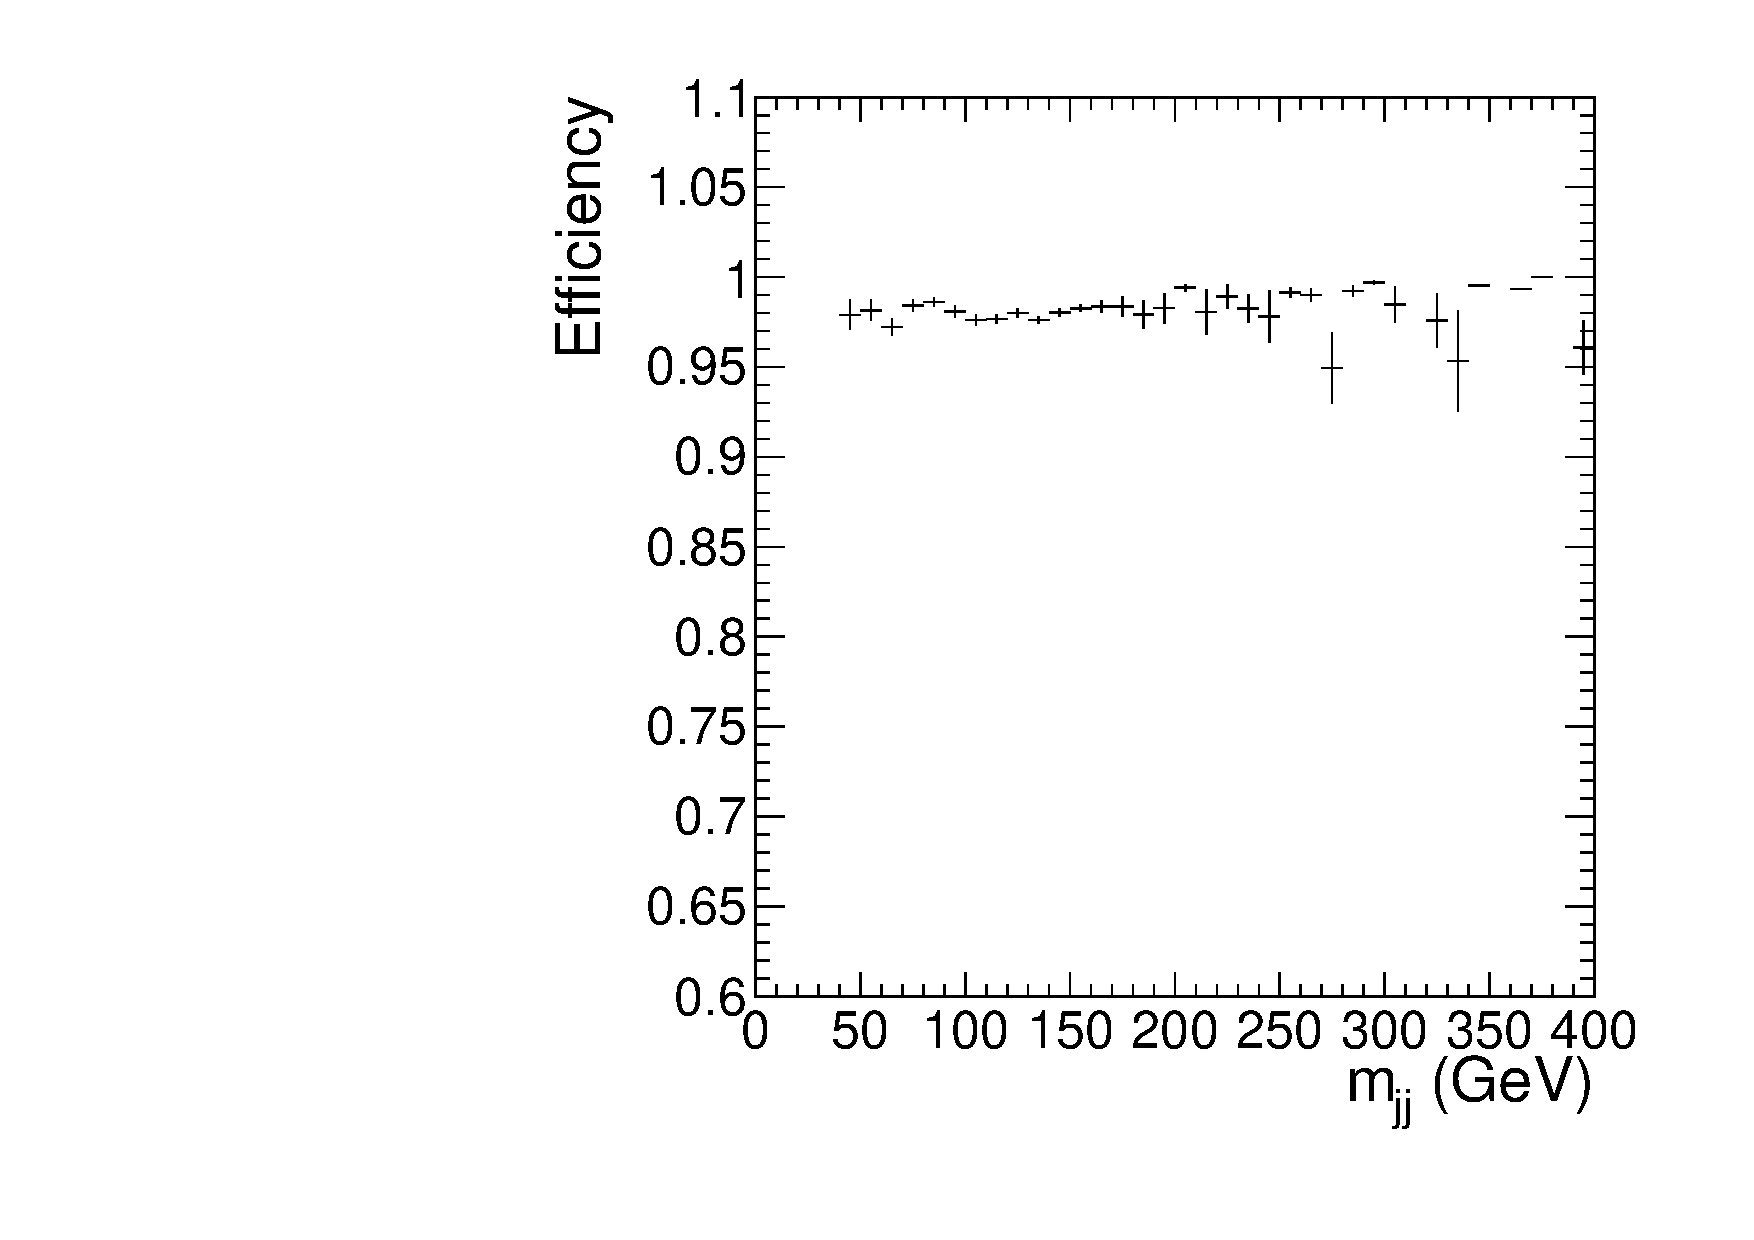
\includegraphics[width=0.4\textwidth]{figs/effPlots/fig_WH_eff_HLTEle2jPfMht_mht.pdf}
   }
   \vspace*{1mm} \\
   \subfigure[]{
   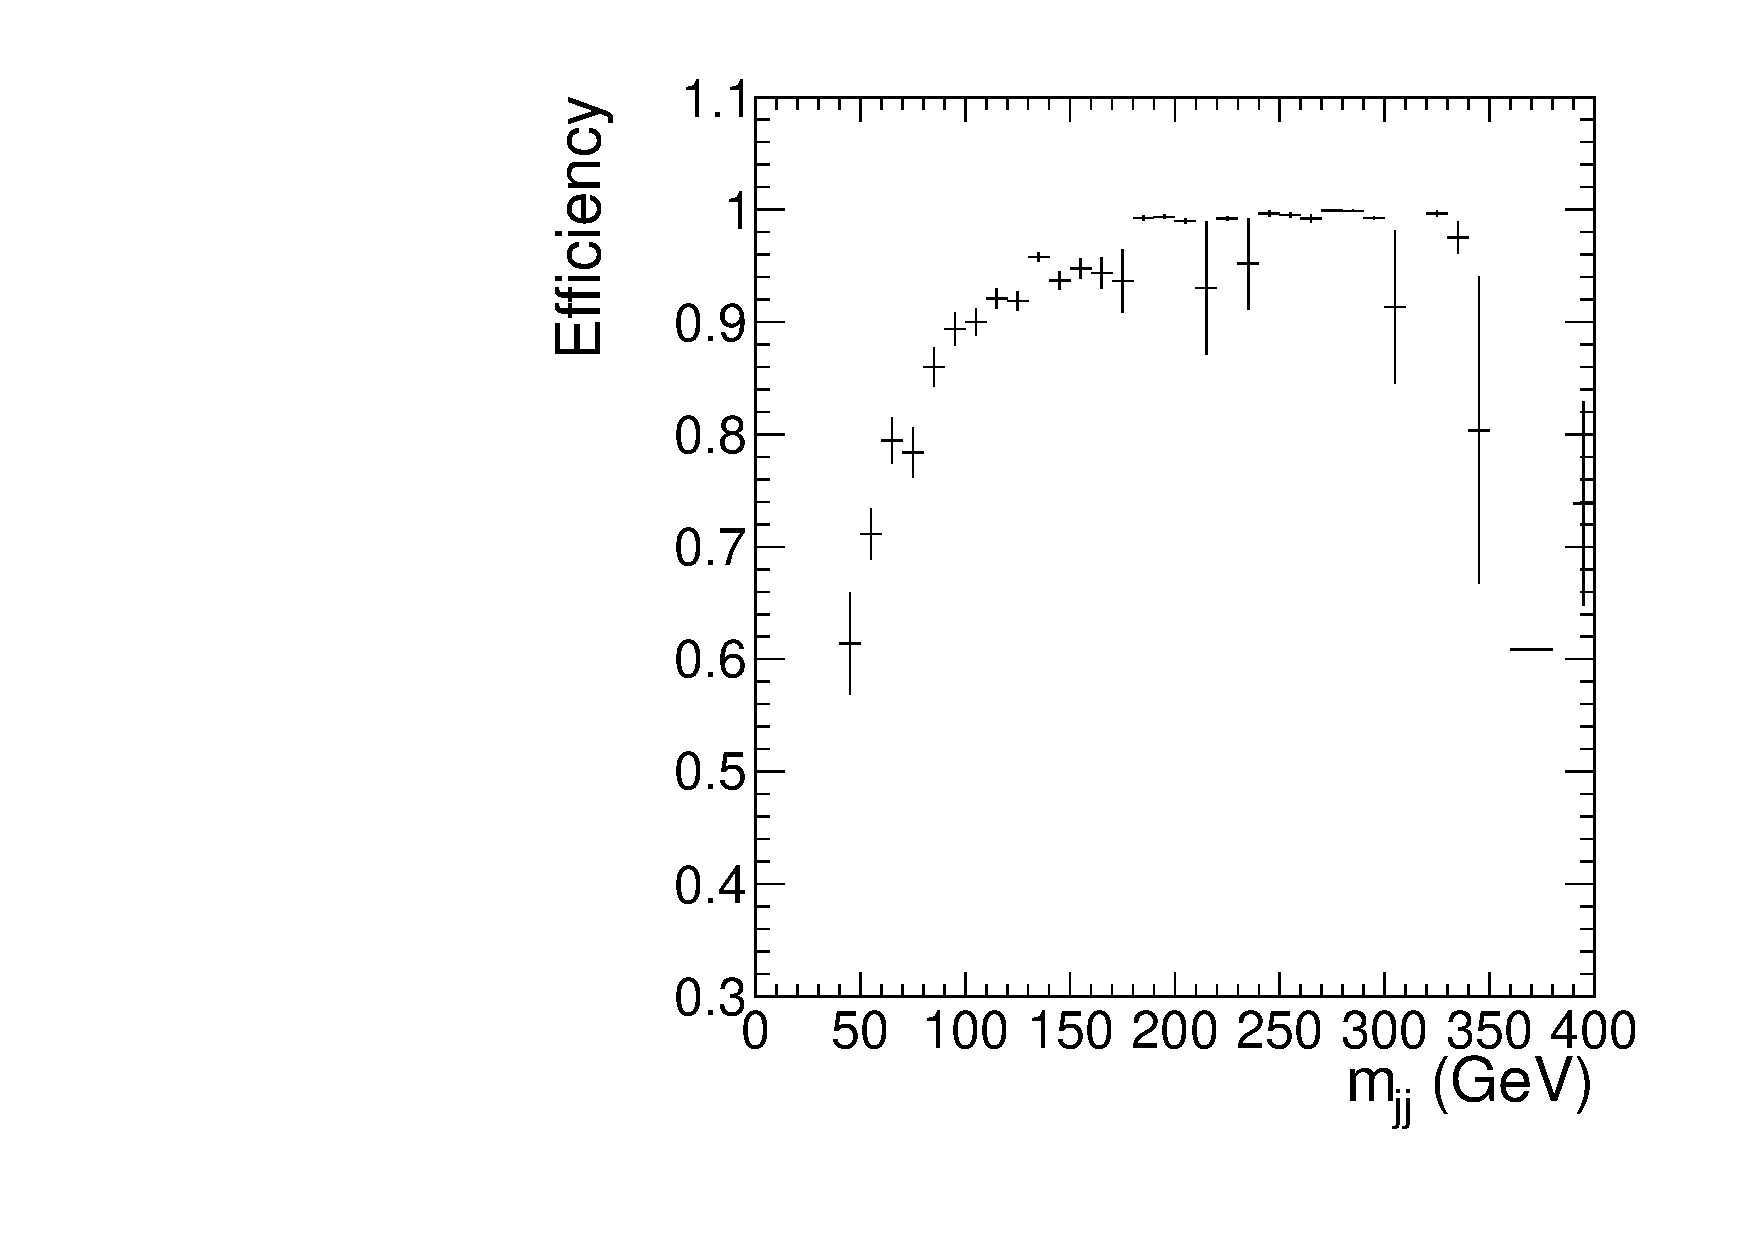
\includegraphics[width=0.4\textwidth]{figs/effPlots/fig_WH_eff_HLTEle2jPfMht_dijet.pdf}
   }
   \subfigure[]{
   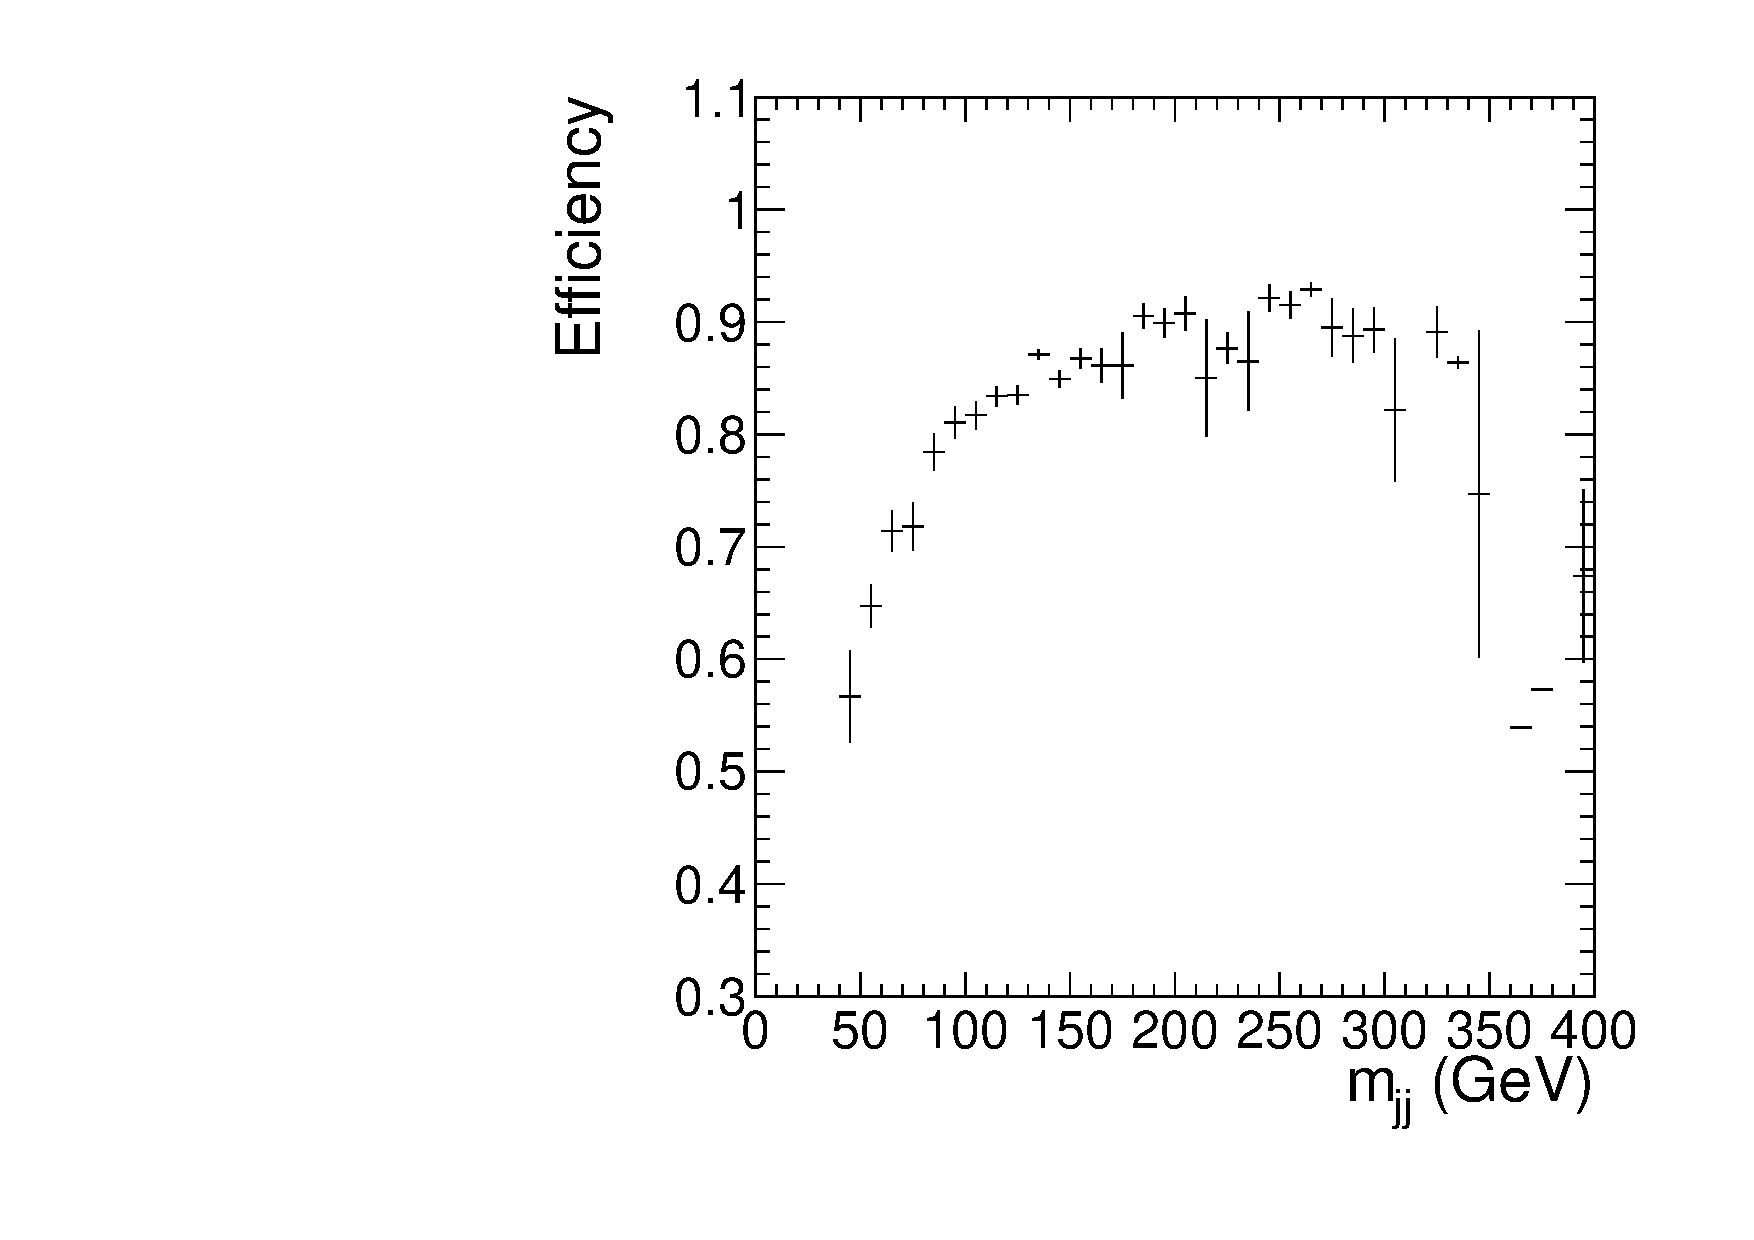
\includegraphics[width=0.4\textwidth]{figs/effPlots/fig_WH_eff_HLTEle2jPfMht_total.pdf}
   }
   \vspace*{1mm} \\
   \subfigure[]{
   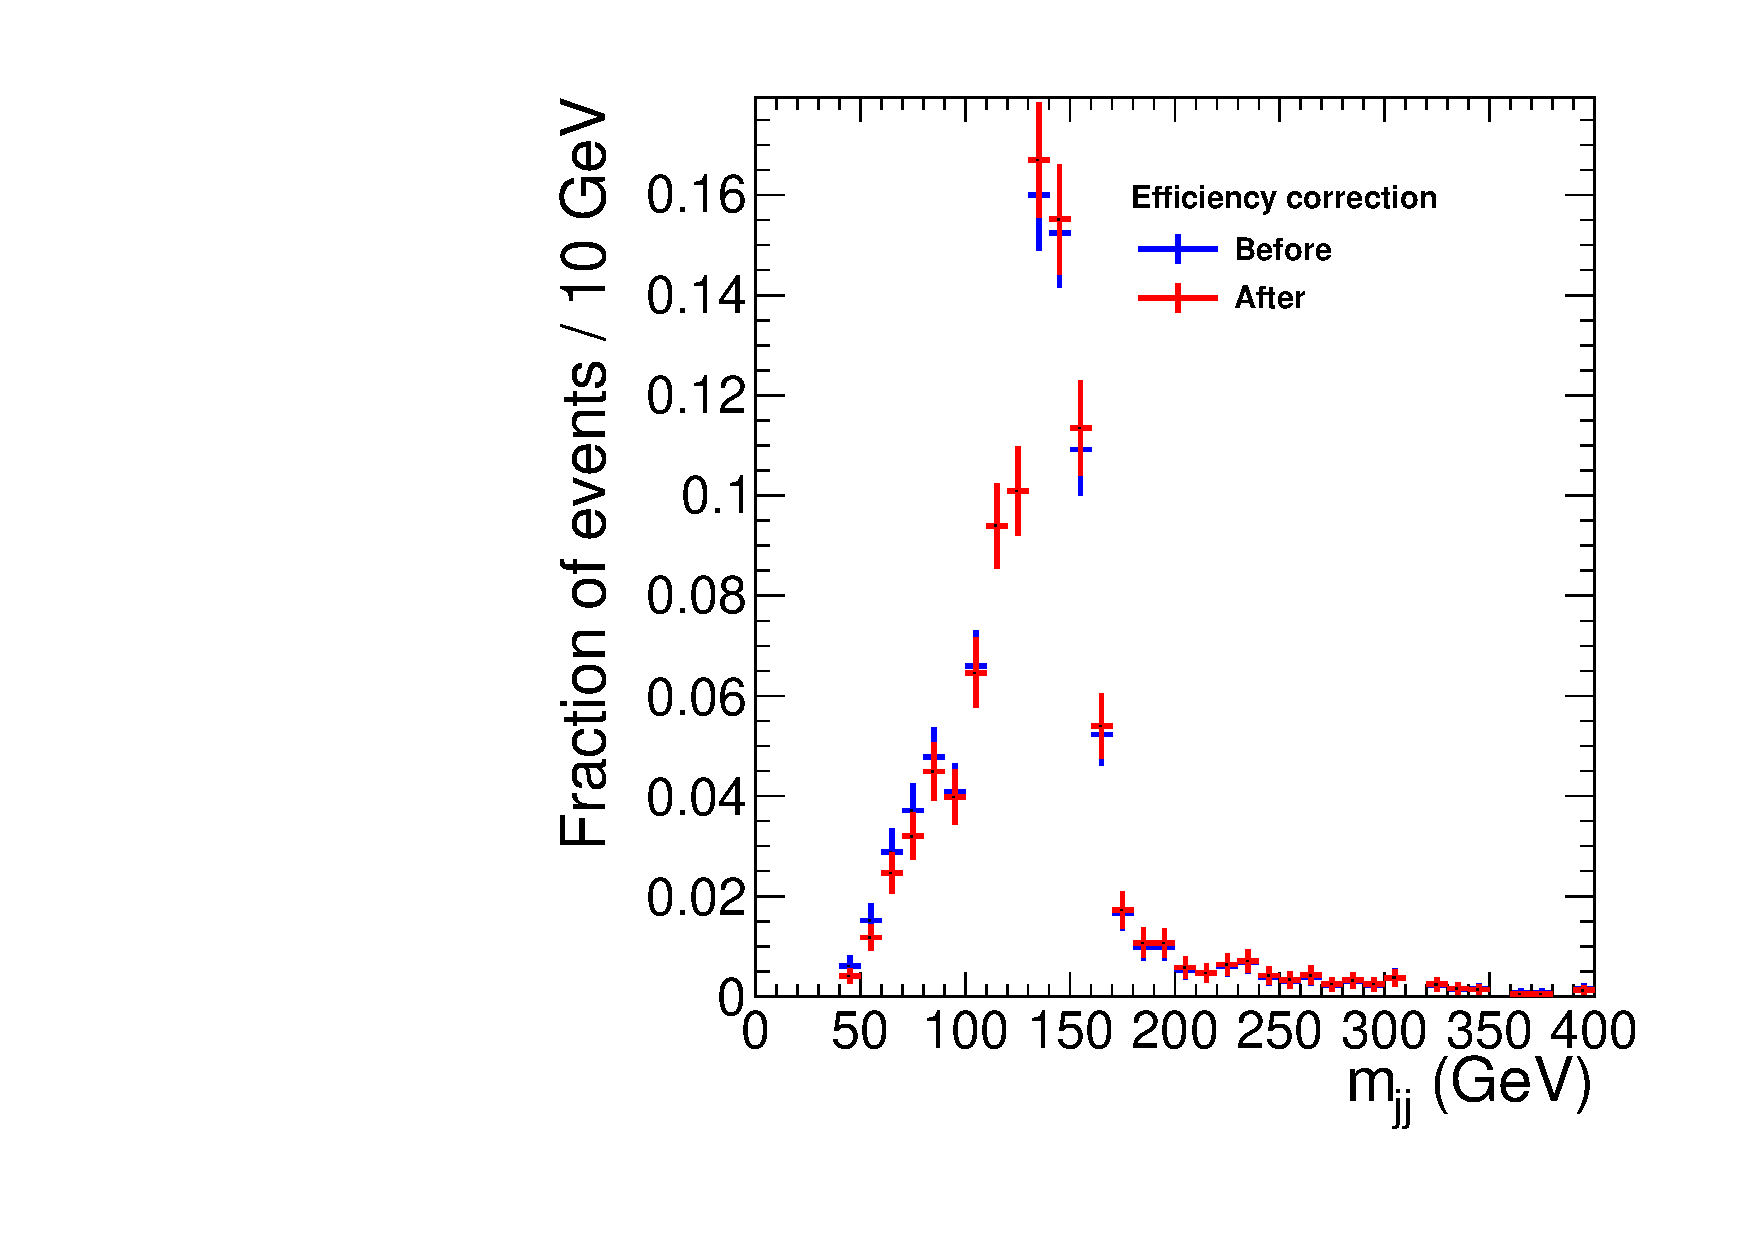
\includegraphics[width=0.4\textwidth]{figs/effPlots/fig_WH_eff_HLTEle2jPfMht_template.pdf}
   }
   \subfigure[]{
   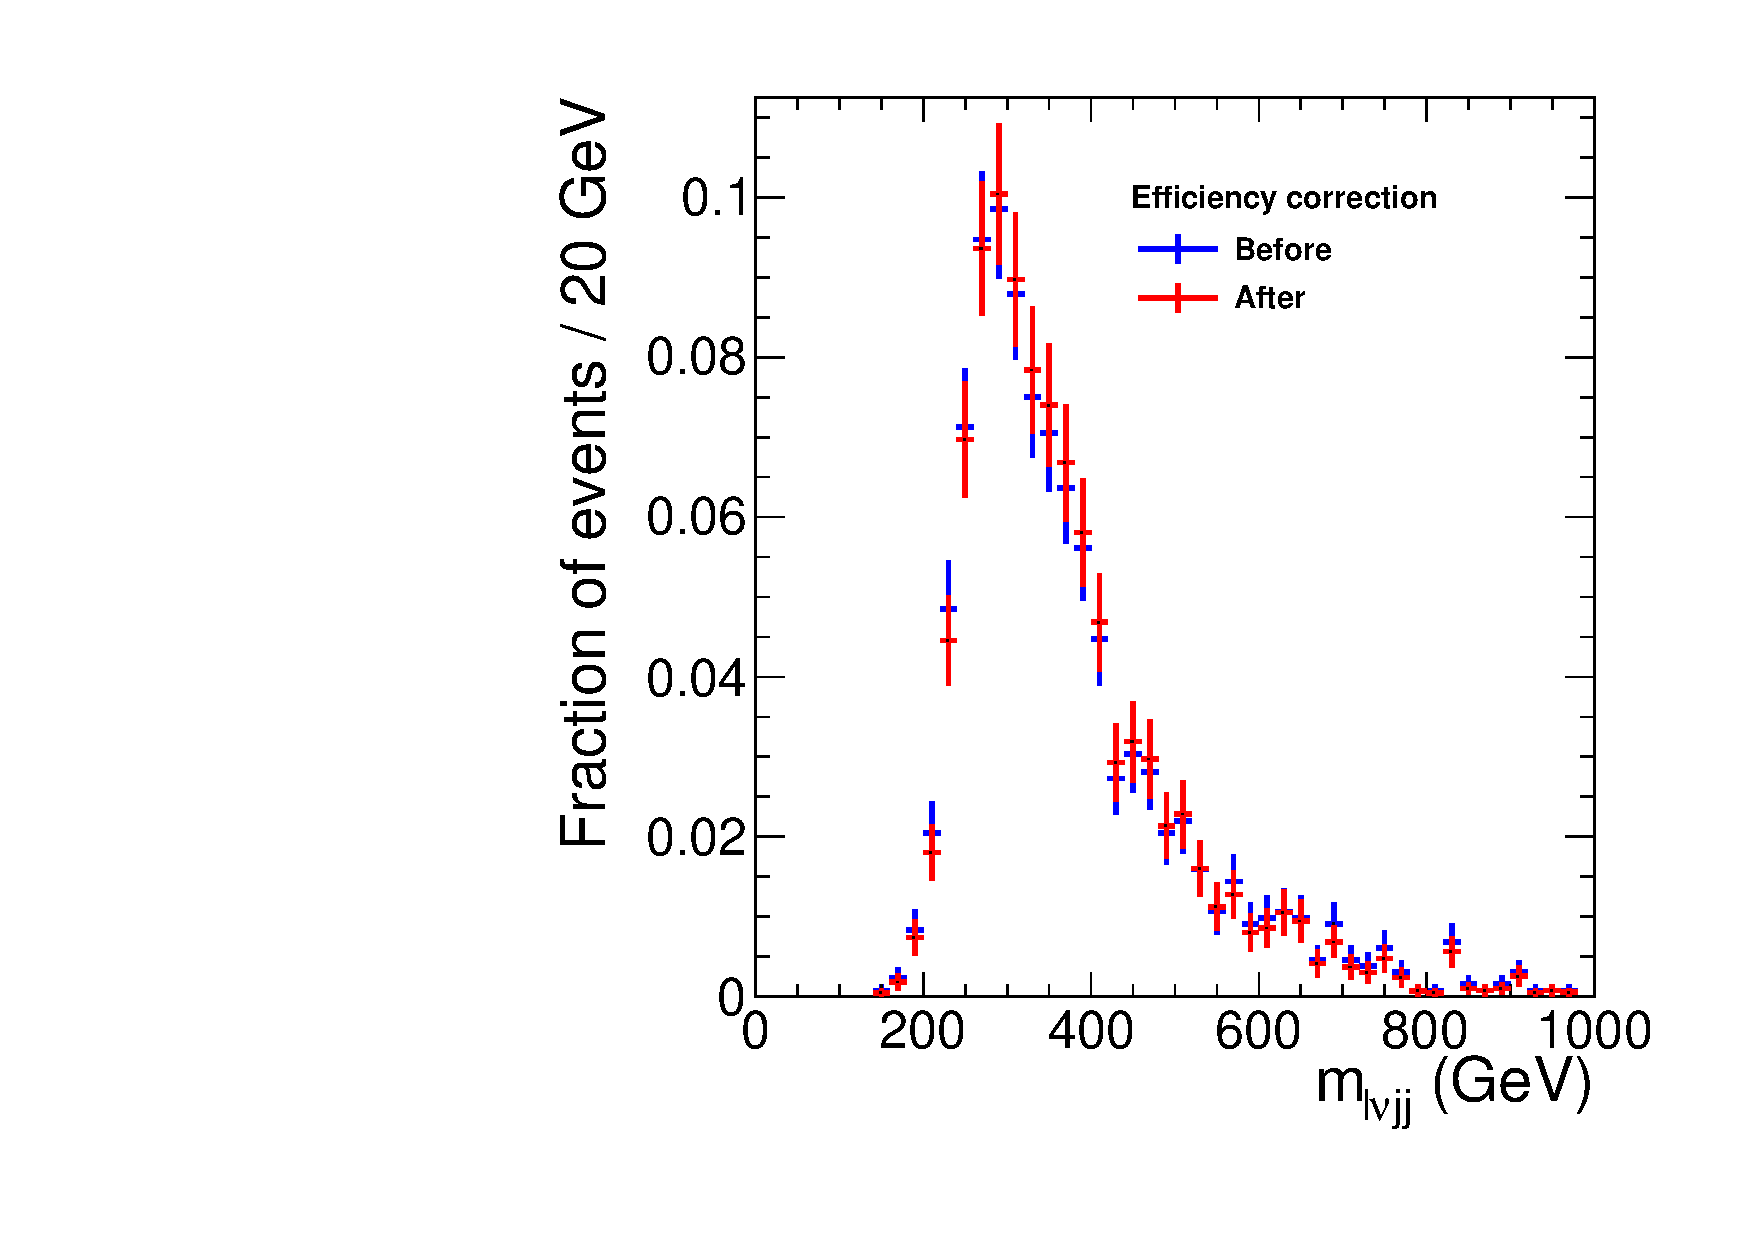
\includegraphics[width=0.4\textwidth]{figs/effPlots/fig_WH_eff_HLTEle2jPfMht_template4body.pdf}
   }
   \caption{For WH signal: Luminosity weighted average trigger efficiency in the 
   electron + 2jet + missing $H_T$ trigger as a function of $m_{jj}$: (a) for the electrong leg, 
   (b) for the missing $H_T$ leg, (c) for the dijet leg, and (d) total, \textit{i.e.}, the product 
   of the efficiencies for the three legs. 
   The effect of this efficiency correction on W+jets shape is shown for 
   $m_{jj}$ (e) and $m_{\ell\nu jj}$ (f) templates.}
\label{fig:EleHadhlteffWH}}
\end{figure}
%%%%%%%%%%%%%%%%%%%%
\clearpage
\subsection{Separation by trigger epochs for this study}
%%%%%%%%%%%%%%%%%%%%
The full dataset ($4.7fb^{-1}$) can be separated into three epochs
\begin{itemize}
\item Single Electron Trigger: The first $215pb^{-1}$.
\item Electron + 2 Jet Trigger, where we use Calorimeter Jets: The next $3820pb^{-1}$.
\item Electron + 2 Jet Trigger, where we use Particle Flow Jets: The last $665pb^{-1}$.
\end{itemize}
In the default fitter the $m_{jj}$ efficiency corrections are applied and all three 
epochs are fitted simultaneously. The results are shown if Fig.~\ref{fig:ElectronFitAllEpochs} 
and a bias can be observed. However, since the efficiency corrections for the data
obtained using the Calorimeter Jet Trigger are still computed for PF Jets, it is plausible
the the corrections are not properly modeled. Thus we separate and fit the data for two 
categories: 
\begin{itemize}
\item with the calorimeter jets used in the trigger (Fig.~\ref{fig:ElectronFitTwoCaloJetEpoch}). A very pronounced bias is seen.
\item without the calorimeter jets (Fig.~\ref{fig:ElectronFitNOTTwoCaloJetEpoch}). The fit produces a reasonable result.
\end{itemize}
Thus, the $3820pb^{-1}$ of data could not be used if we took this approach.


\begin{figure}
\begin{center}
  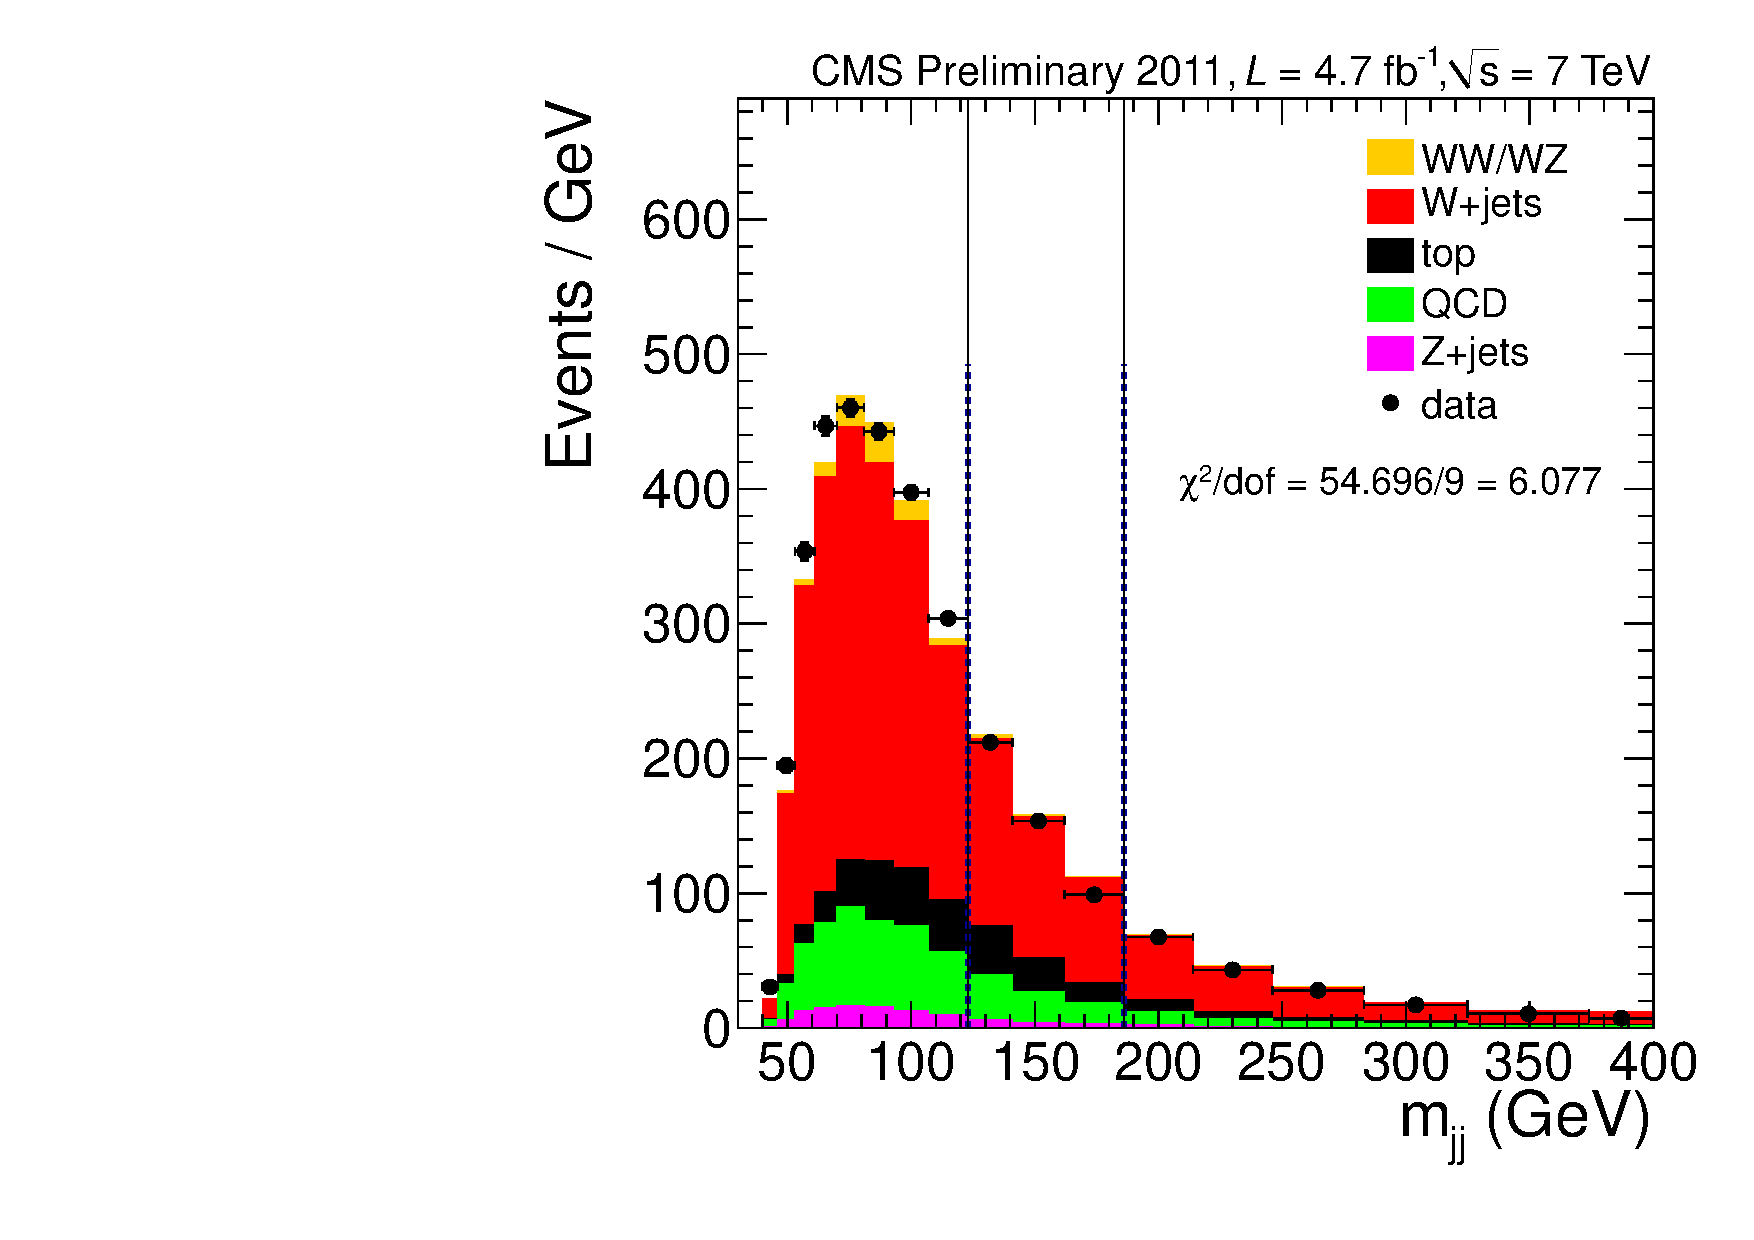
\includegraphics[width=0.45\textwidth]{figs/ElectronFitAllEpochs_Wjj_Mjj_Electron_2jets_Stacked.pdf}
  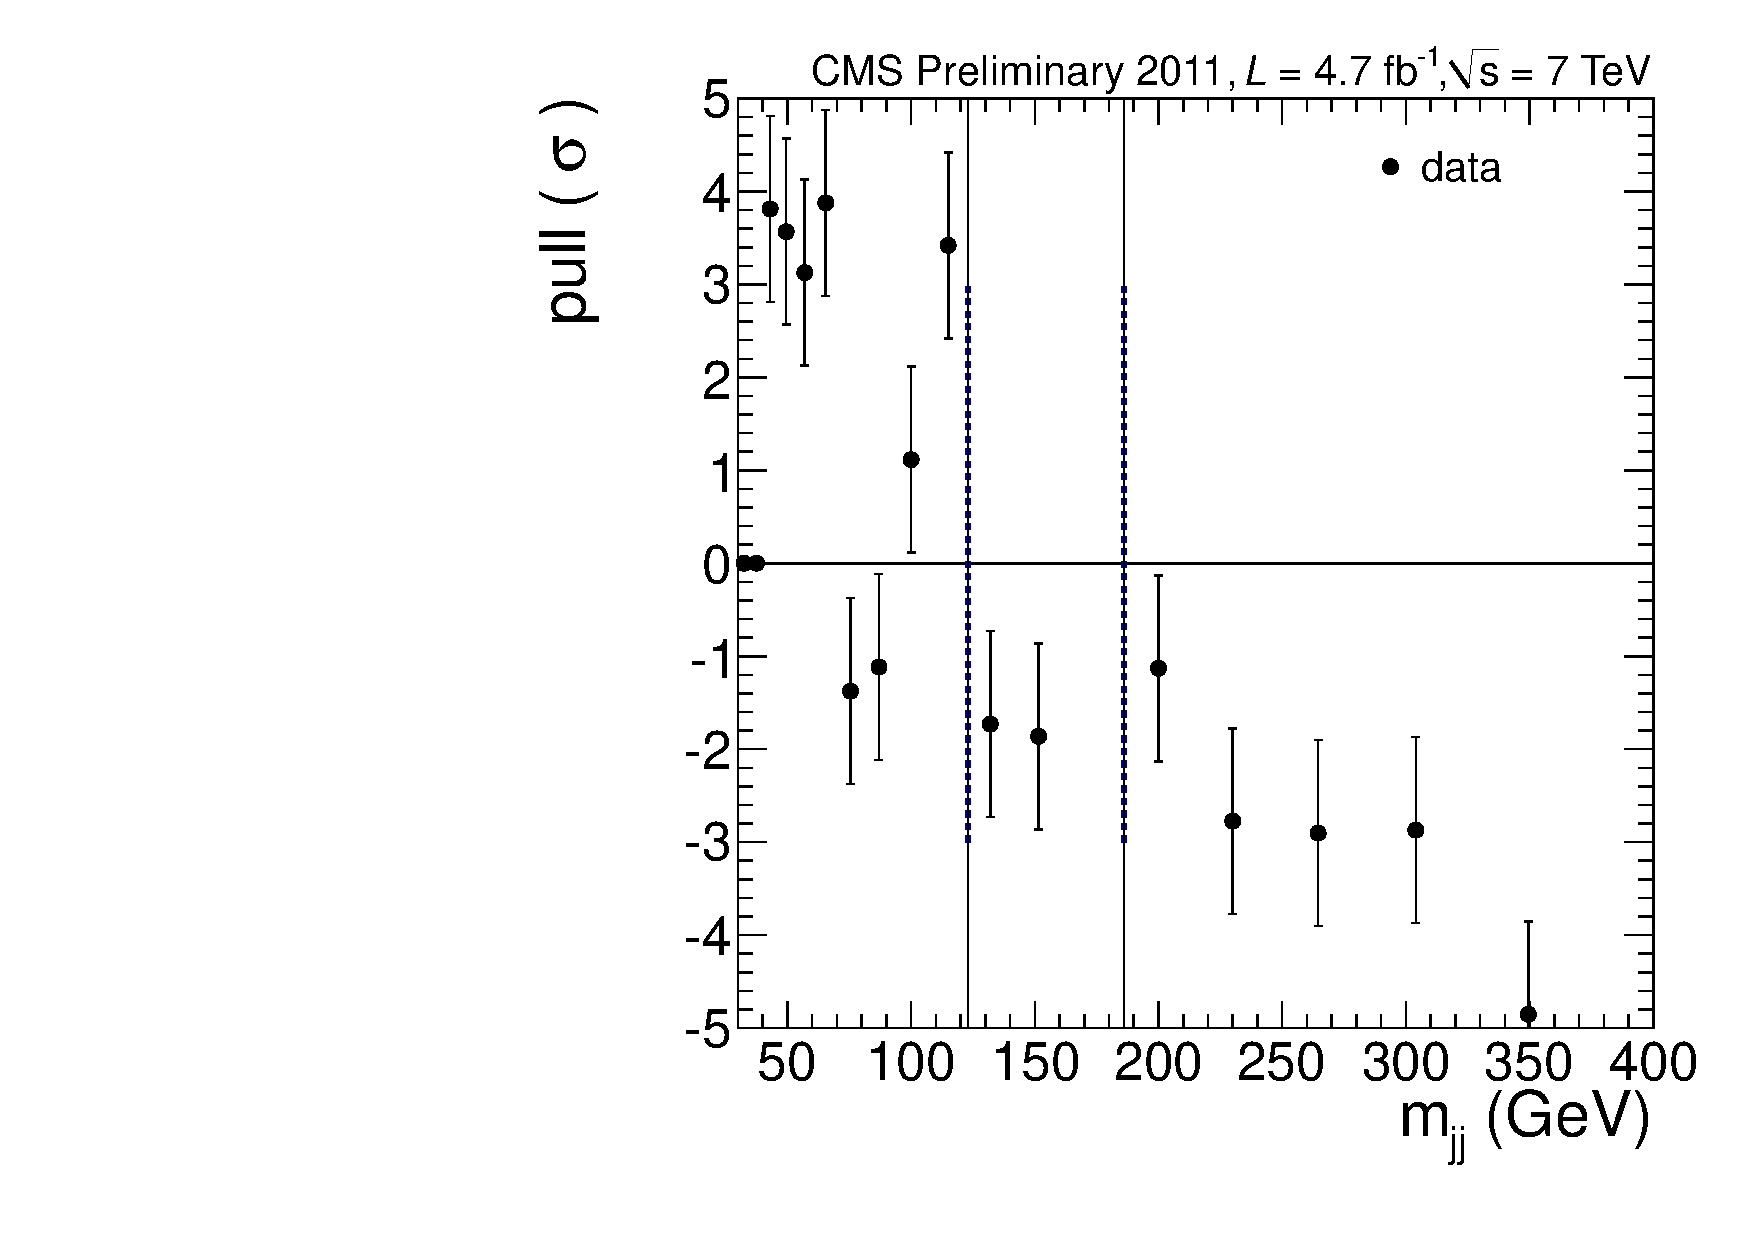
\includegraphics[width=0.45\textwidth]{figs/ElectronFitAllEpochs_Wjj_Mjj_Electron_2jets_Pull.pdf}
\end{center}
\caption{\label{fig:ElectronFitAllEpochs}Standard Fit to the $4.7fb^{-1}$ of data (in the 2Jet Bin).}
\end {figure}


\begin{figure}
\begin{center}
  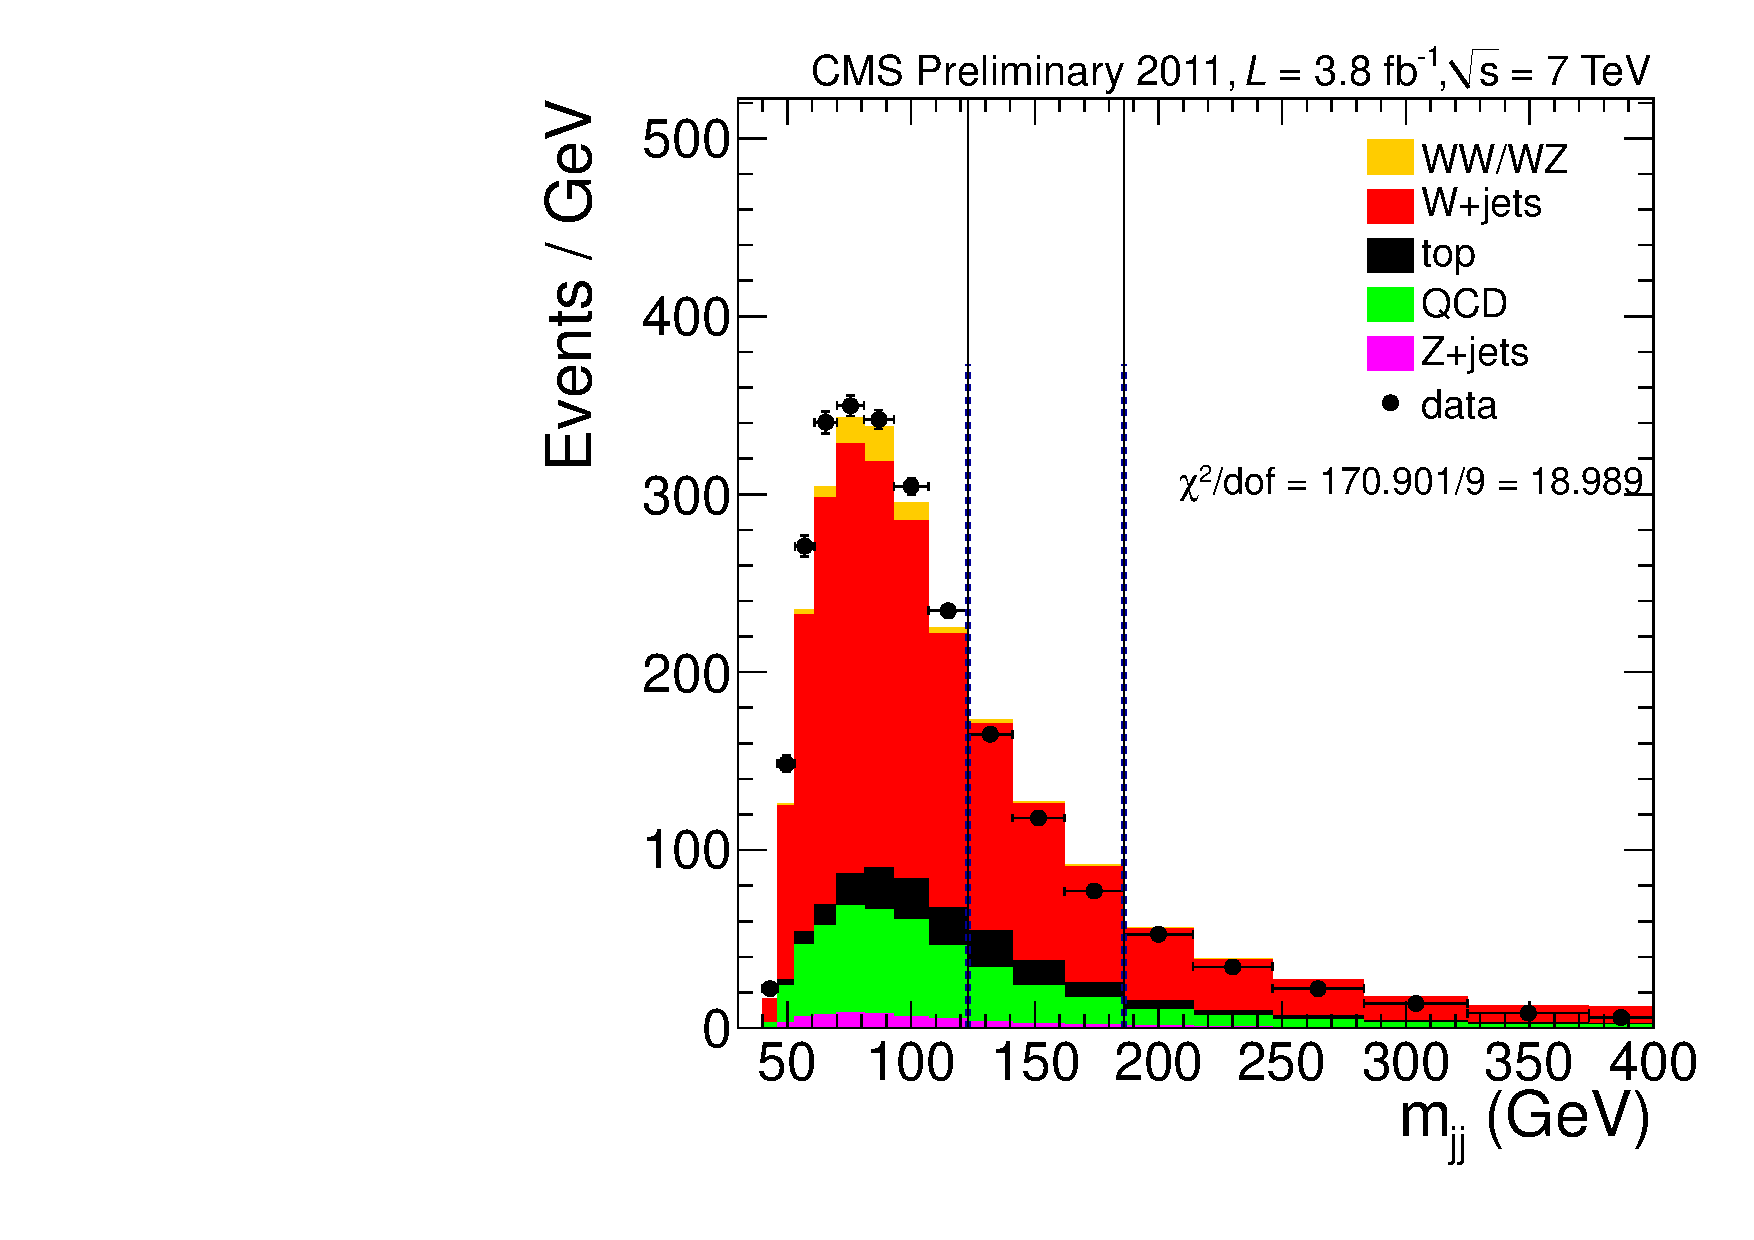
\includegraphics[width=0.45\textwidth]{figs/ElectronFitTwoCaloJetEpoch_Wjj_Mjj_Electron_2jets_Stacked.pdf}
  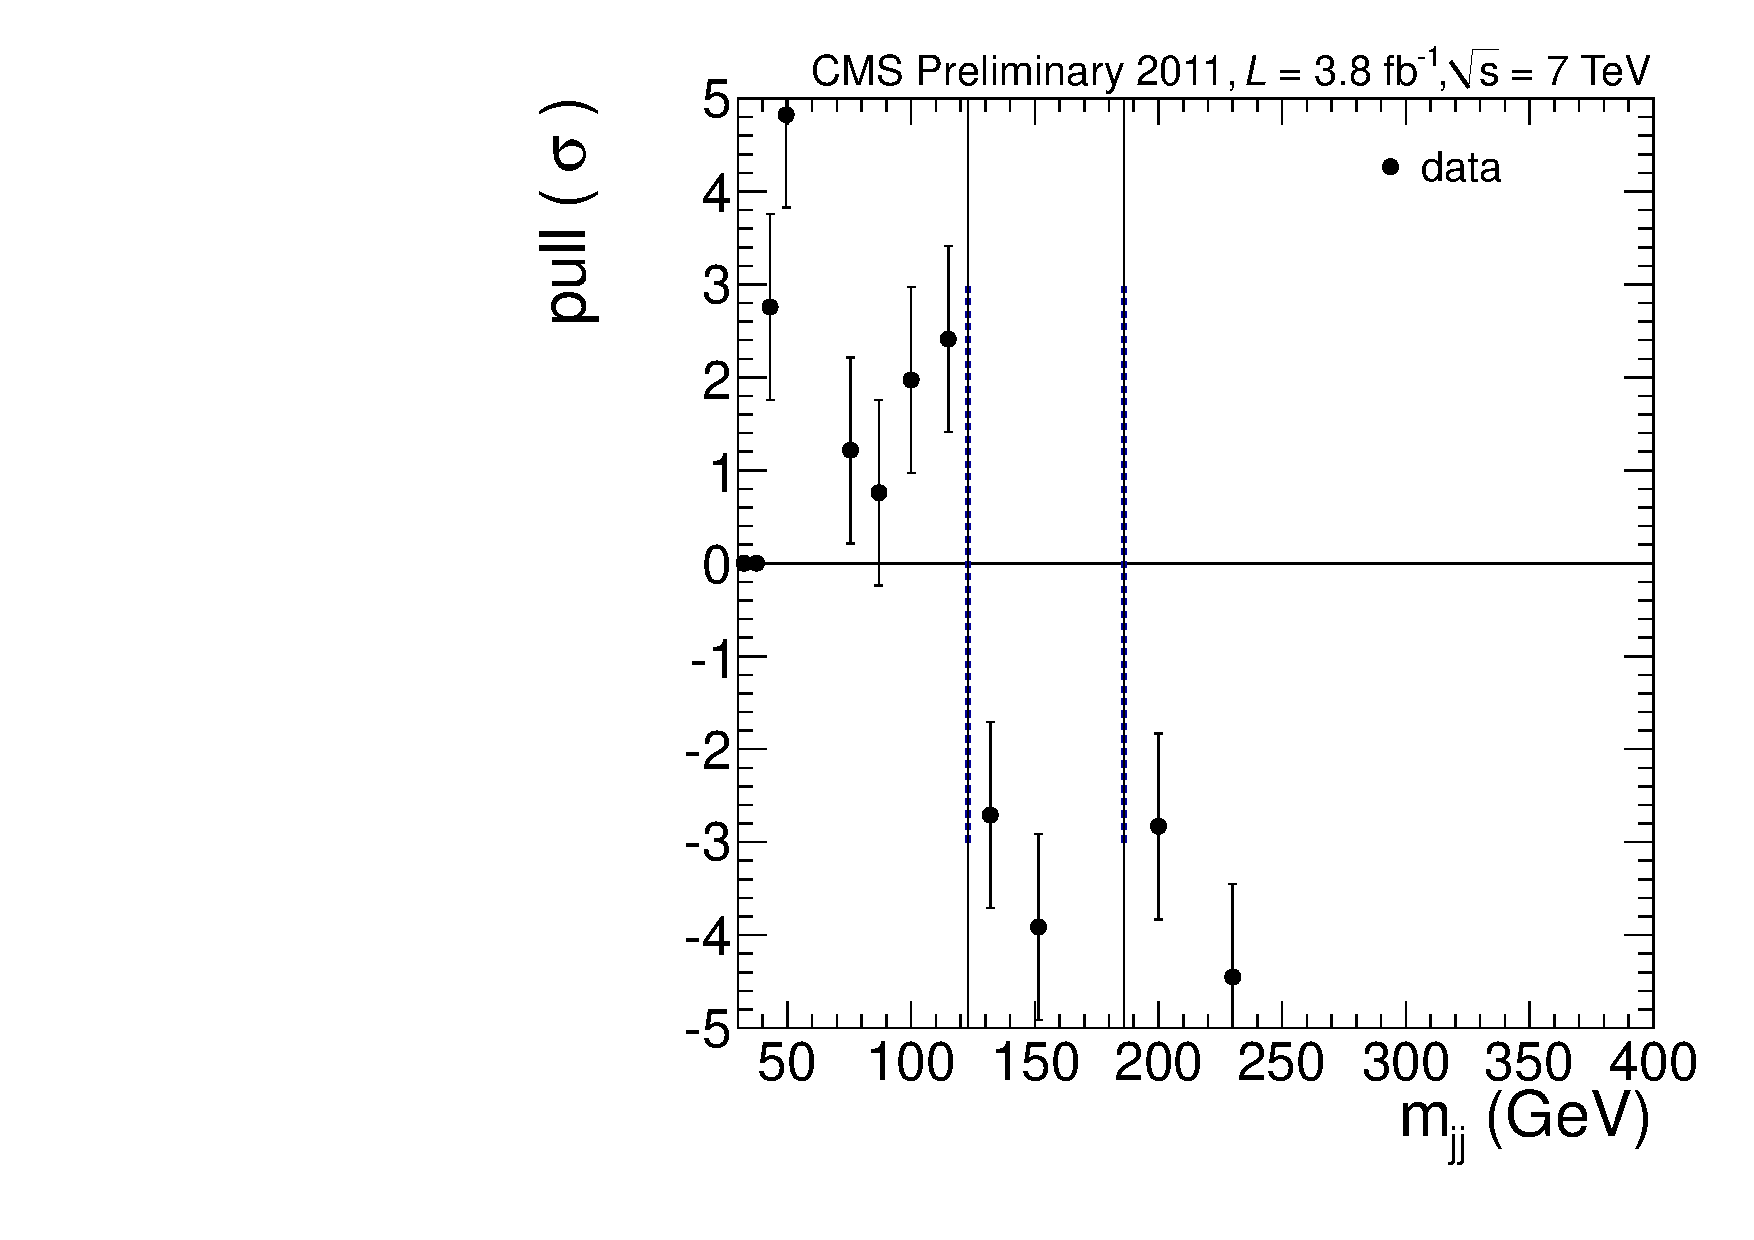
\includegraphics[width=0.45\textwidth]{figs/ElectronFitTwoCaloJetEpoch_Wjj_Mjj_Electron_2jets_Pull.pdf}
\end{center}
\caption{\label{fig:ElectronFitTwoCaloJetEpoch}Fit to the $3820pb^{-1}$ of data, where the 2 Jet Calorimeter Trigger was used (in the 2Jet Bin).}
\end {figure}


\begin{figure}
\begin{center}
  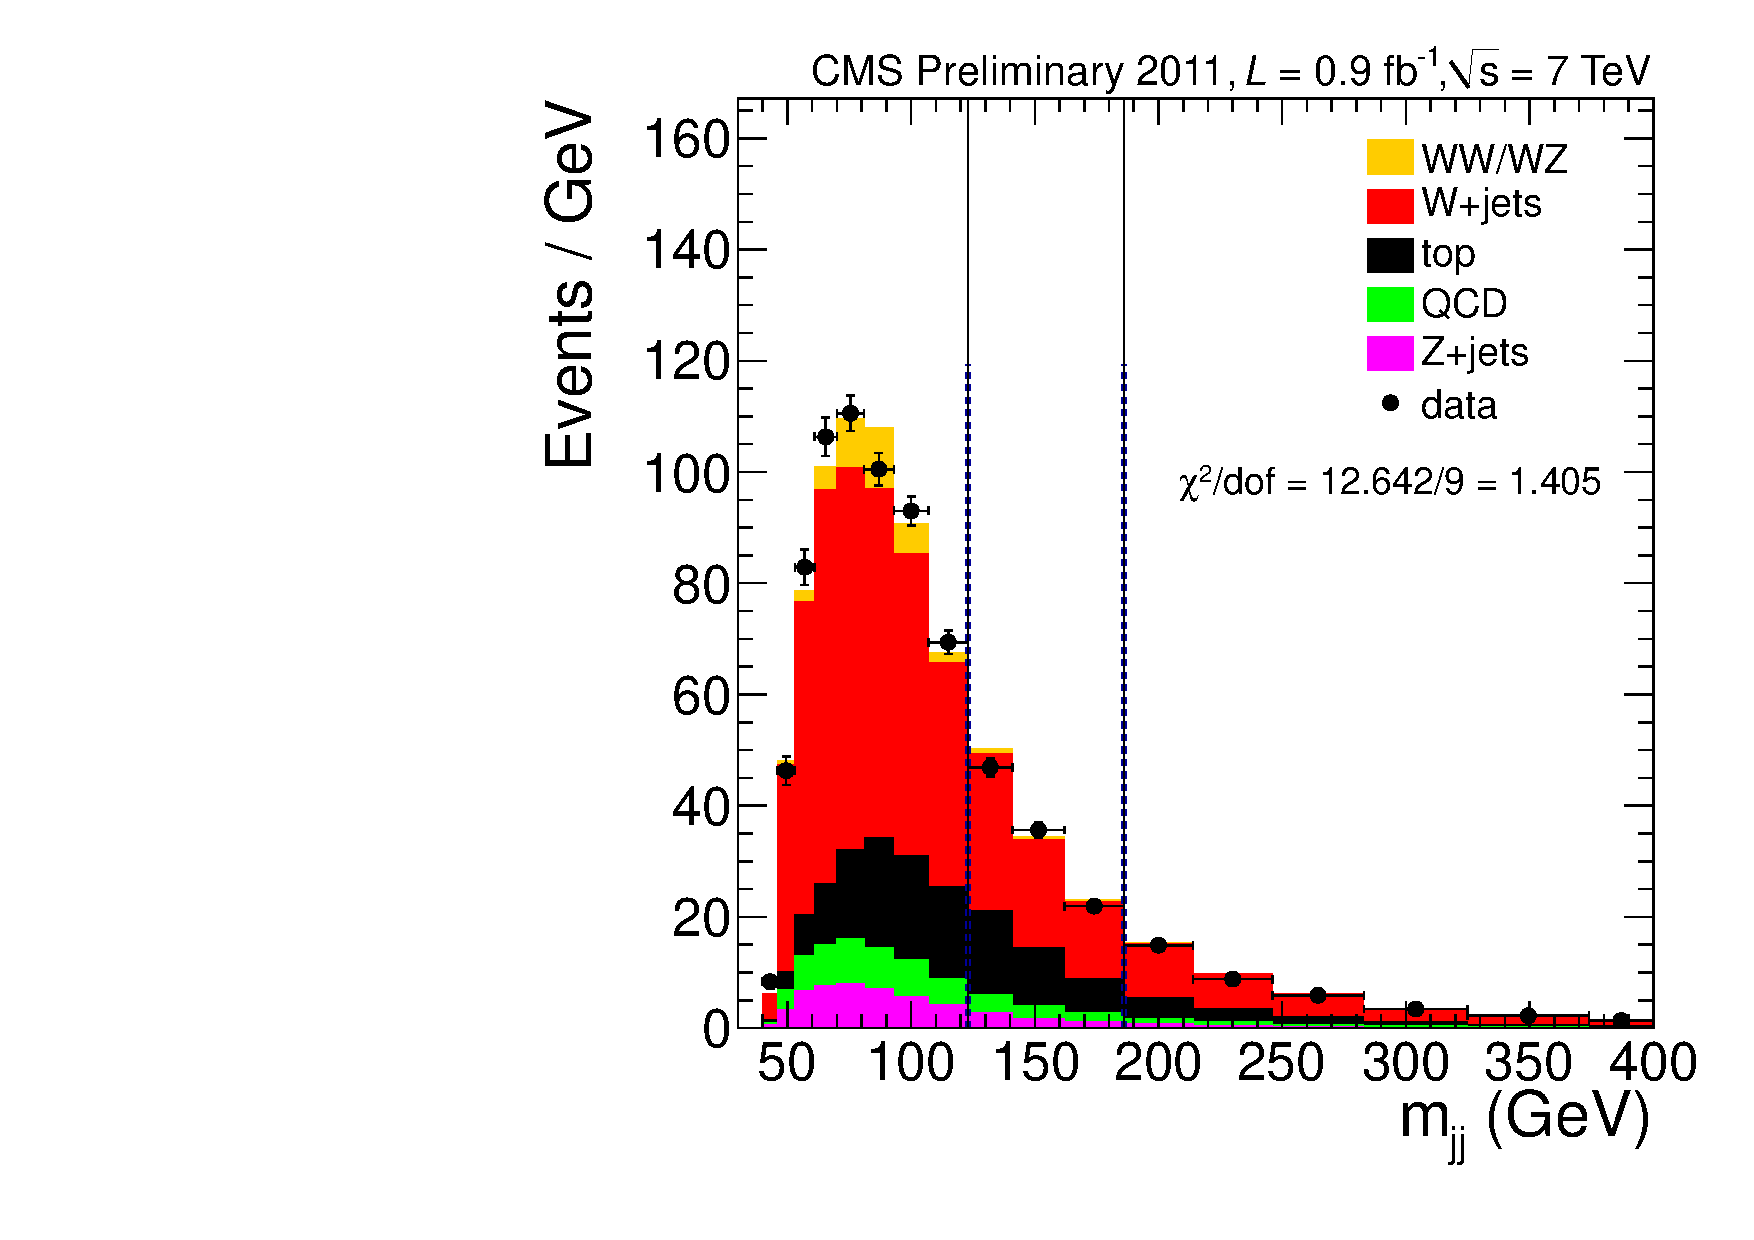
\includegraphics[width=0.45\textwidth]{figs/ElectronFitNOTTwoCaloJetEpoch_Wjj_Mjj_Electron_2jets_Stacked.pdf}
  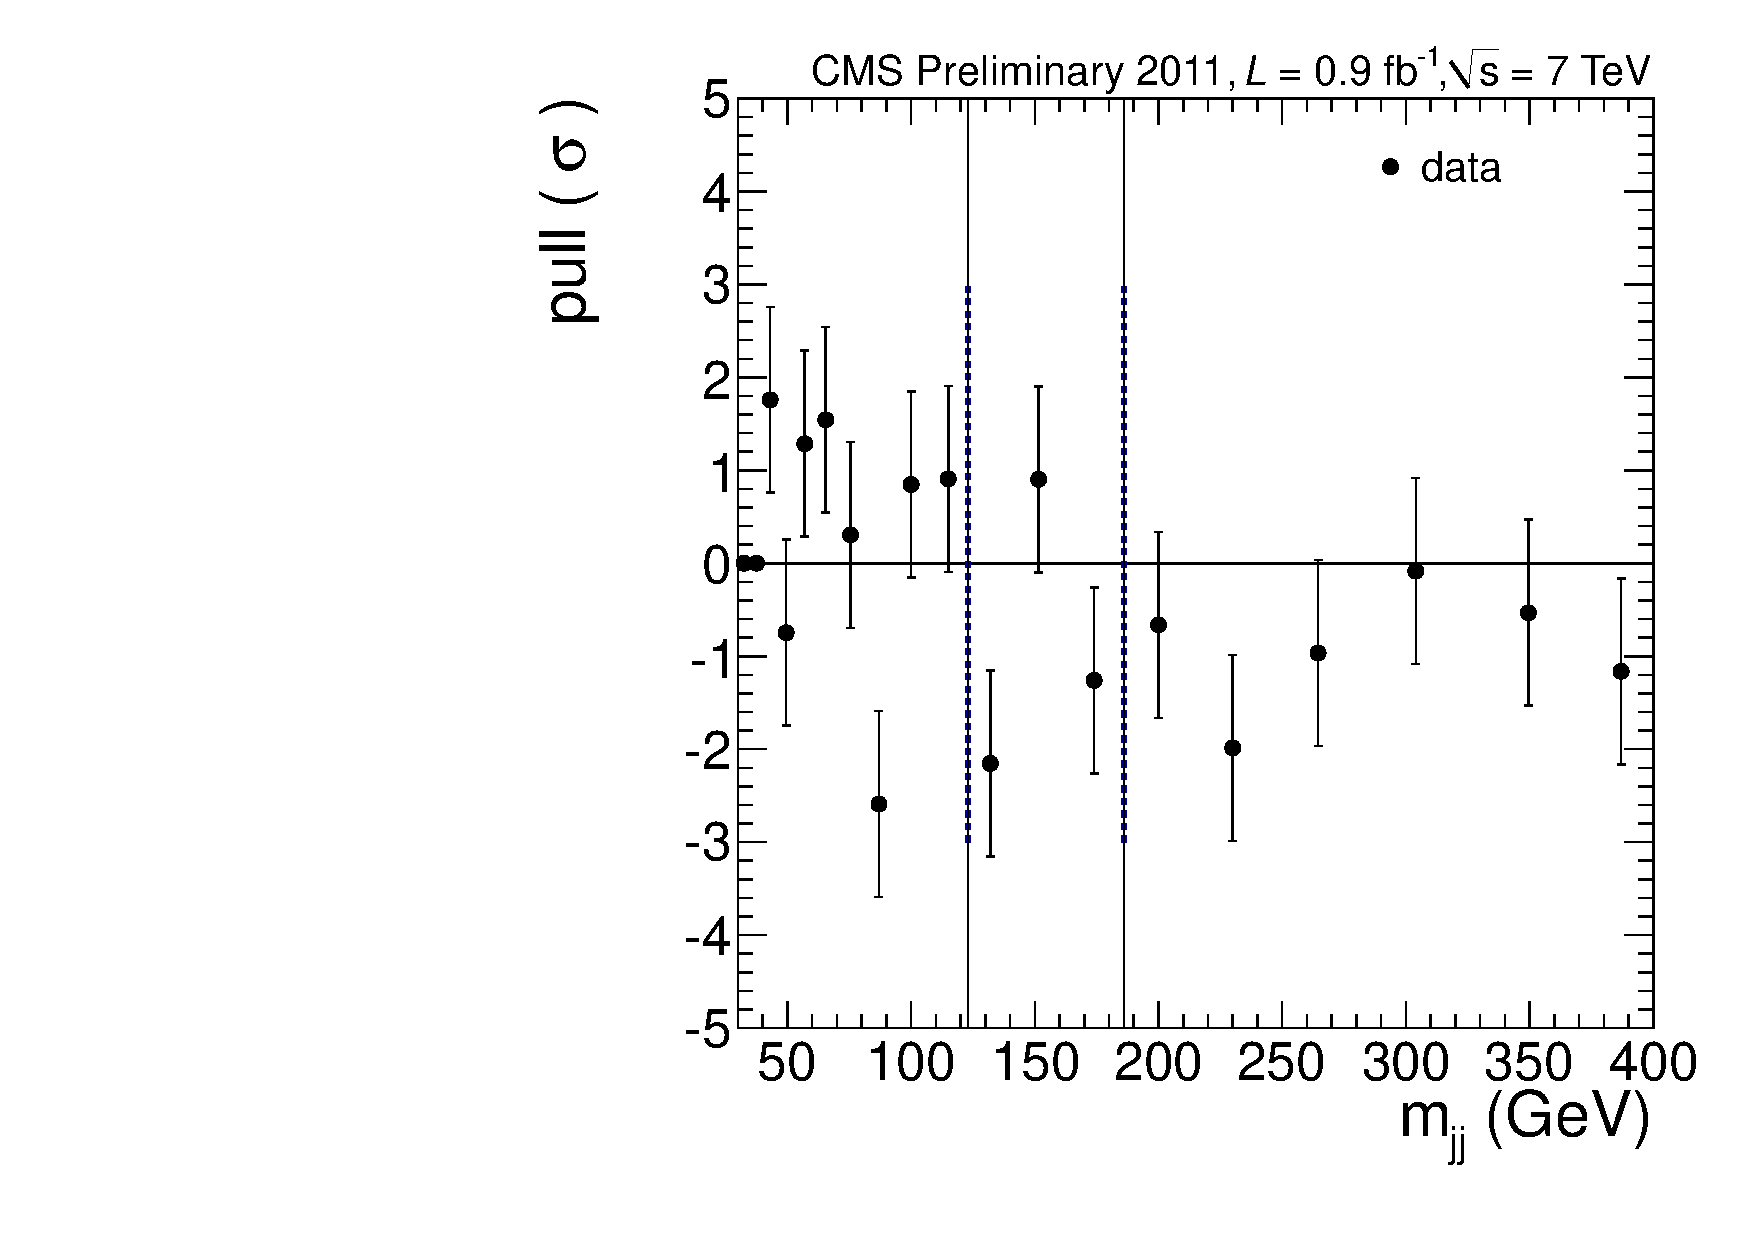
\includegraphics[width=0.45\textwidth]{figs/ElectronFitNOTTwoCaloJetEpoch_Wjj_Mjj_Electron_2jets_Pull.pdf}
\end{center}
\caption{\label{fig:ElectronFitNOTTwoCaloJetEpoch}Fit to the $215+665pb^{-1}$ of data, where the 2 Jet Calorimeter Trigger was not used (in the 2Jet Bin).}
\end {figure}


\clearpage
\subsection{Conclusion of the study on Electron + 2 jets + missing $H_T$ trigger}
%%%%%%%%%%%%%%%%%%%%
We presently cannot reliably model the efficiency of the ElectronHad triggers for the 
$3.8~fb^{-1}$ of 2011B data where CaloJet was used in the trigger.
The data with PFJet in the trigger are well modeled, as we 
have verified in the last $800~pb^{-1}$ of 2011B data sample.
Therefore, we should be fine using the ElectronHad triggers 
in 2012 because they will use PFJet.
For the present round of analysis we will have to rely 
on the SingleElectron triggers with an increase in the 
offline $E_T$ threshold to 35 GeV.


\clearpage


%\clearpage
%\section{Conclusions}
\label{sec:conclusions}
We have studied the electroweak production 
of two heavy gauge bosons  in events 
with a leptonically decaying W boson and exactly two jets.
The analyzed dataset 
corresponds to an integrated luminosity of 5.0~fb${}^{-1}$ at 
$\sqrt{s} = 7$~TeV collected by the CMS detector at the Large Hadron Collider.
With the kinematic requirements imposed in the analysis, we 
observe 2979 $\pm$ 361 (stat) $\pm$ 402 (syst) WW+WZ events, 
in agreement with the Standard Model expectation. 
The measured value of the sum of WW and WZ cross sections is 
66.7 $\pm$ 8.1 (stat) $\pm$ 8.5 (syst) pb, consistent 
with the standard model prediction of 65.6~pb. 
This is the first observation of diboson events in 
the semi-leptonic final state in a pp collider.
We derive limits on anomalous triple gauge couplings  
using the $p_T$ distribution of the dijet system: 
$ -0.038 < \lambda_Z < 0.030$, 
$ -0.111 < \Delta{\kappa_\gamma} < 0.142$.
These limits are the most stringent at a hadron collider to-date 
and are approaching the sensitivity of combined LEP measurements.


%%%%%%%%%%%%%%%%%%%%%%%%%%%%%%%%%%%%%%%%%%%%%%%%%%%%%%%%%%%%%%%%%%%%%%%%%%

% >> acknowledgements (for journal papers)
% Please include the latest version from https://twiki.cern.ch/twiki/bin/viewauth/CMS/Internal/PubAcknow.
%\section*{Acknowledgements}
% ack-text

%% **DO NOT REMOVE BIBLIOGRAPHY**
\bibliography{auto_generated}   % will be created by the tdr script.

%%%% DO NOT ADD \end{document}!

